% Options for packages loaded elsewhere
\PassOptionsToPackage{unicode}{hyperref}
\PassOptionsToPackage{hyphens}{url}
%
\documentclass[
]{article}
\usepackage{amsmath,amssymb}
\usepackage{lmodern}
\usepackage{iftex}
\ifPDFTeX
  \usepackage[T1]{fontenc}
  \usepackage[utf8]{inputenc}
  \usepackage{textcomp} % provide euro and other symbols
\else % if luatex or xetex
  \usepackage{unicode-math}
  \defaultfontfeatures{Scale=MatchLowercase}
  \defaultfontfeatures[\rmfamily]{Ligatures=TeX,Scale=1}
\fi
% Use upquote if available, for straight quotes in verbatim environments
\IfFileExists{upquote.sty}{\usepackage{upquote}}{}
\IfFileExists{microtype.sty}{% use microtype if available
  \usepackage[]{microtype}
  \UseMicrotypeSet[protrusion]{basicmath} % disable protrusion for tt fonts
}{}
\makeatletter
\@ifundefined{KOMAClassName}{% if non-KOMA class
  \IfFileExists{parskip.sty}{%
    \usepackage{parskip}
  }{% else
    \setlength{\parindent}{0pt}
    \setlength{\parskip}{6pt plus 2pt minus 1pt}}
}{% if KOMA class
  \KOMAoptions{parskip=half}}
\makeatother
\usepackage{xcolor}
\usepackage{longtable,booktabs,array}
\usepackage{multirow}
\usepackage{calc} % for calculating minipage widths
% Correct order of tables after \paragraph or \subparagraph
\usepackage{etoolbox}
\makeatletter
\patchcmd\longtable{\par}{\if@noskipsec\mbox{}\fi\par}{}{}
\makeatother
% Allow footnotes in longtable head/foot
\IfFileExists{footnotehyper.sty}{\usepackage{footnotehyper}}{\usepackage{footnote}}
\makesavenoteenv{longtable}
\usepackage{graphicx}
\makeatletter
\def\maxwidth{\ifdim\Gin@nat@width>\linewidth\linewidth\else\Gin@nat@width\fi}
\def\maxheight{\ifdim\Gin@nat@height>\textheight\textheight\else\Gin@nat@height\fi}
\makeatother
% Scale images if necessary, so that they will not overflow the page
% margins by default, and it is still possible to overwrite the defaults
% using explicit options in \includegraphics[width, height, ...]{}
\setkeys{Gin}{width=\maxwidth,height=\maxheight,keepaspectratio}
% Set default figure placement to htbp
\makeatletter
\def\fps@figure{htbp}
\makeatother
\setlength{\emergencystretch}{3em} % prevent overfull lines
\providecommand{\tightlist}{%
  \setlength{\itemsep}{0pt}\setlength{\parskip}{0pt}}
\setcounter{secnumdepth}{-\maxdimen} % remove section numbering
\ifLuaTeX
  \usepackage{selnolig}  % disable illegal ligatures
\fi
\IfFileExists{bookmark.sty}{\usepackage{bookmark}}{\usepackage{hyperref}}
\IfFileExists{xurl.sty}{\usepackage{xurl}}{} % add URL line breaks if available
\urlstyle{same} % disable monospaced font for URLs
\hypersetup{
  hidelinks,
  pdfcreator={LaTeX via pandoc}}

\author{}
\date{}

\begin{document}


\includegraphics[width=1.03533in,height=1.0133in]{images/media/image11.png}

\textbf{UNIVERSITAS INDONESIA}

\textbf{LLM-Assisted Knowledge Graph Completion untuk Pemetaan
Interkoneksi Materi Sains (Fisika, Kimia, Biologi) pada Kurikulum
Merdeka Kelas XII}

\textbf{SKRIPSI}

\begin{longtable}[]{@{}
  >{\raggedright\arraybackslash}p{(\columnwidth - 2\tabcolsep) * \real{0.6659}}
  >{\raggedright\arraybackslash}p{(\columnwidth - 2\tabcolsep) * \real{0.3341}}@{}}
\toprule()
\begin{minipage}[b]{\linewidth}\raggedright
\textbf{FADRIAN YHOGA PRATAMA}
\end{minipage} & \begin{minipage}[b]{\linewidth}\raggedright
\textbf{2206819395}
\end{minipage} \\
\begin{minipage}[b]{\linewidth}\raggedright
\textbf{SOROS FEBRIANO}
\end{minipage} & \begin{minipage}[b]{\linewidth}\raggedright
\textbf{2206083445}
\end{minipage} \\
\begin{minipage}[b]{\linewidth}\raggedright
\textbf{TEGAR WAHYU KHISBULLOH}
\end{minipage} & \begin{minipage}[b]{\linewidth}\raggedright
\textbf{2206082032}
\end{minipage} \\
\midrule()
\endhead
\bottomrule()
\end{longtable}

\textbf{FAKULTAS ILMU KOMPUTER}

\textbf{PROGRAM STUDI ILMU KOMPUTER}

\textbf{DEPOK}

\textbf{JUNI 2026}


\includegraphics[width=1.03533in,height=1.0133in]{images/media/image11.png}

\textbf{UNIVERSITAS INDONESIA}

\textbf{LLM-Assisted Knowledge Graph Completion untuk Pemetaan
Interkoneksi Materi Sains (Fisika, Kimia, Biologi) pada Kurikulum
Merdeka Tingkat SMA}

\textbf{SKRIPSI}

\textbf{Diajukan sebagai salah satu syarat memperoleh gelar}

\textbf{Sarjana Ilmu Komputer}

\begin{longtable}[]{@{}
  >{\raggedright\arraybackslash}p{(\columnwidth - 2\tabcolsep) * \real{0.6659}}
  >{\raggedright\arraybackslash}p{(\columnwidth - 2\tabcolsep) * \real{0.3341}}@{}}
\toprule()
\begin{minipage}[b]{\linewidth}\raggedright
\textbf{FADRIAN YHOGA PRATAMA}
\end{minipage} & \begin{minipage}[b]{\linewidth}\raggedright
\textbf{2206819395}
\end{minipage} \\
\begin{minipage}[b]{\linewidth}\raggedright
\textbf{SOROS FEBRIANO}
\end{minipage} & \begin{minipage}[b]{\linewidth}\raggedright
\textbf{2206083445}
\end{minipage} \\
\begin{minipage}[b]{\linewidth}\raggedright
\textbf{TEGAR WAHYU KHISBULLOH}
\end{minipage} & \begin{minipage}[b]{\linewidth}\raggedright
\textbf{2206082032}
\end{minipage} \\
\midrule()
\endhead
\bottomrule()
\end{longtable}

\textbf{FAKULTAS ILMU KOMPUTER}

\textbf{PROGRAM STUDI ILMU KOMPUTER}

\textbf{DEPOK}

\textbf{JUNI 2026}

\hypertarget{halaman-pernyataan-orisinalitas}{%
\section{HALAMAN PERNYATAAN
ORISINALITAS}\label{halaman-pernyataan-orisinalitas}}

\textbf{Tugas Akhir ini adalah hasil karya saya sendiri, dan semua
sumber baik yang dikutip maupun dirujuk telah saya nyatakan dengan
benar.}

\begin{longtable}[]{@{}
  >{\raggedright\arraybackslash}p{(\columnwidth - 2\tabcolsep) * \real{0.2282}}
  >{\raggedright\arraybackslash}p{(\columnwidth - 2\tabcolsep) * \real{0.7718}}@{}}
\toprule()
\begin{minipage}[b]{\linewidth}\raggedright
\textbf{Nama}
\end{minipage} & \begin{minipage}[b]{\linewidth}\raggedright
: Fadrian Yhoga Pratama, Soros Febriano, Tegar Wahyu Khisbulloh
\end{minipage} \\
\begin{minipage}[b]{\linewidth}\raggedright
\textbf{NPM}
\end{minipage} & \begin{minipage}[b]{\linewidth}\raggedright
: 2206819395, 2206083445, 2206082032
\end{minipage} \\
\begin{minipage}[b]{\linewidth}\raggedright
\textbf{Tanda Tangan}
\end{minipage} & \begin{minipage}[b]{\linewidth}\raggedright
:
\end{minipage} \\
\begin{minipage}[b]{\linewidth}\raggedright
\textbf{Tanggal}
\end{minipage} & \begin{minipage}[b]{\linewidth}\raggedright
: 7 Desember 2026
\end{minipage} \\
\midrule()
\endhead
\bottomrule()
\end{longtable}

\hypertarget{halaman-pernyataan-penggunaan-kecerdasan-artifisial}{%
\section{HALAMAN PERNYATAAN PENGGUNAAN KECERDASAN
ARTIFISIAL}\label{halaman-pernyataan-penggunaan-kecerdasan-artifisial}}

\textbf{Saya menyatakan bahwa dalam penyusunan Tugas Akhir ini, saya
menggunakan teknologi Kecerdasan Buatan dengan platform ChatGPT dan
Gemini untuk tujuan pemeriksaan dan perbaikan tata bahasa dan saya
bertanggung jawab penuh atas keakuratan, orisinalitas, dan integritas
seluruh isi Tugas Akhir ini.}

\begin{longtable}[]{@{}
  >{\raggedright\arraybackslash}p{(\columnwidth - 2\tabcolsep) * \real{0.2282}}
  >{\raggedright\arraybackslash}p{(\columnwidth - 2\tabcolsep) * \real{0.7718}}@{}}
\toprule()
\begin{minipage}[b]{\linewidth}\raggedright
\textbf{Nama}
\end{minipage} & \begin{minipage}[b]{\linewidth}\raggedright
: Fadrian Yhoga Pratama, Soros Febriano, Tegar Wahyu Khisbulloh
\end{minipage} \\
\begin{minipage}[b]{\linewidth}\raggedright
\textbf{NPM}
\end{minipage} & \begin{minipage}[b]{\linewidth}\raggedright
: 2206819395, 2206083445, 2206082032
\end{minipage} \\
\begin{minipage}[b]{\linewidth}\raggedright
\textbf{Tanda Tangan}
\end{minipage} & \begin{minipage}[b]{\linewidth}\raggedright
:
\end{minipage} \\
\begin{minipage}[b]{\linewidth}\raggedright
\textbf{Tanggal}
\end{minipage} & \begin{minipage}[b]{\linewidth}\raggedright
: 7 Desember 2026
\end{minipage} \\
\midrule()
\endhead
\bottomrule()
\end{longtable}

\hypertarget{halaman-pengesahan}{%
\section{HALAMAN PENGESAHAN}\label{halaman-pengesahan}}

\begin{longtable}[]{@{}
  >{\raggedright\arraybackslash}p{(\columnwidth - 2\tabcolsep) * \real{0.3725}}
  >{\raggedright\arraybackslash}p{(\columnwidth - 2\tabcolsep) * \real{0.6275}}@{}}
\toprule()
\multicolumn{2}{@{}>{\raggedright\arraybackslash}p{(\columnwidth - 2\tabcolsep) * \real{1.0000} + 2\tabcolsep}@{}}{%
\begin{minipage}[b]{\linewidth}\raggedright
Tugas Akhir ini diajukan oleh :
\end{minipage}} \\
\begin{minipage}[b]{\linewidth}\raggedright
Nama/NPM Mahasiswa 1
\end{minipage} & \begin{minipage}[b]{\linewidth}\raggedright
: Fadrian Yhoga Pratama/2206819395
\end{minipage} \\
\begin{minipage}[b]{\linewidth}\raggedright
Nama/NPM Mahasiswa 2
\end{minipage} & \begin{minipage}[b]{\linewidth}\raggedright
: Soros Febriano/2206083445
\end{minipage} \\
\begin{minipage}[b]{\linewidth}\raggedright
Nama/NPM Mahasiswa 3
\end{minipage} & \begin{minipage}[b]{\linewidth}\raggedright
: Tegar Wahyu Khisbulloh/2206082032
\end{minipage} \\
\begin{minipage}[b]{\linewidth}\raggedright
Program Studi
\end{minipage} & \begin{minipage}[b]{\linewidth}\raggedright
: Sarjana Ilmu Komputer
\end{minipage} \\
\begin{minipage}[b]{\linewidth}\raggedright
Judul
\end{minipage} & \begin{minipage}[b]{\linewidth}\raggedright
: LLM-Assisted Knowledge Graph Completion untuk Pemetaan Interkoneksi
Materi Sains (Fisika, Kimia, Biologi) pada Kurikulum Merdeka Tingkat SMA
\end{minipage} \\
\midrule()
\endhead
\bottomrule()
\end{longtable}

\textbf{Telah berhasil dipertahankan di hadapan Dewan Penguji dan
diterima sebagai bagian persyaratan yang diperlukan untuk memperoleh
gelar Sarjana Ilmu Komputer pada Program Studi Sarjana Ilmu Komputer,
Fakultas Ilmu Komputer, Universitas Indonesia}

\textbf{DEWAN PENGUJI}

\begin{longtable}[]{@{}
  >{\raggedright\arraybackslash}p{(\columnwidth - 4\tabcolsep) * \real{0.2324}}
  >{\raggedright\arraybackslash}p{(\columnwidth - 4\tabcolsep) * \real{0.4030}}
  >{\raggedright\arraybackslash}p{(\columnwidth - 4\tabcolsep) * \real{0.3647}}@{}}
\toprule()
\begin{minipage}[b]{\linewidth}\raggedright
Pembimbing :
\end{minipage} & \begin{minipage}[b]{\linewidth}\raggedright
Dr. Siti Aminah, S.Kom., M.Kom.
\end{minipage} & \begin{minipage}[b]{\linewidth}\raggedright
\end{minipage} \\
\begin{minipage}[b]{\linewidth}\raggedright
Pembimbing :
\end{minipage} & \begin{minipage}[b]{\linewidth}\raggedright
\end{minipage} & \begin{minipage}[b]{\linewidth}\raggedright
\end{minipage} \\
\begin{minipage}[b]{\linewidth}\raggedright
Penguji :
\end{minipage} & \begin{minipage}[b]{\linewidth}\raggedright
\end{minipage} & \begin{minipage}[b]{\linewidth}\raggedright
\end{minipage} \\
\begin{minipage}[b]{\linewidth}\raggedright
Penguji :
\end{minipage} & \begin{minipage}[b]{\linewidth}\raggedright
\end{minipage} & \begin{minipage}[b]{\linewidth}\raggedright
\end{minipage} \\
\midrule()
\endhead
\bottomrule()
\end{longtable}

Ditetapkan di : Depok, Jawa Barat

Tanggal :

\hypertarget{kata-pengantar}{%
\section{KATA PENGANTAR}\label{kata-pengantar}}

Puji syukur saya panjatkan kepada Tuhan Yang Maha Esa, karena atas
berkat dan

rahmat-Nya, saya dapat menyelesaikan skripsi ini. Penulisan skripsi ini
dilakukan

dalam rangka memenuhi salah satu syarat untuk mencapai gelar Sarjana
Ekonomi

Jurusan Manajemen pada Fakultas Ekonomi Universitas Indonesia. Saya
menyadari

bahwa, tanpa bantuan dan bimbingan dari berbagai pihak, dari masa
perkuliahan

sampai pada penyusunan skripsi ini, sangatlah sulit bagi saya untuk
menyelesaikan

skripsi ini. Oleh karena itu, saya mengucapkan terima kasih kepada:

(1) Drs. A, selaku dosen pembimbing yang telah menyediakan waktu,
tenaga, dan

pikiran untuk mengarahkan saya dalam penyusunan skripsi ini;

(2) pihak X Company yang telah banyak membantu dalam usaha memperoleh
data

yang saya perlukan;

(3) orang tua dan keluarga saya yang telah memberikan bantuan dukungan
material

dan moral; dan

(4) sahabat yang telah banyak membantu saya dalam menyelesaikan skripsi
ini.

Akhir kata, saya berharap Tuhan Yang Maha Esa berkenan membalas segala
kebaikan

semua pihak yang telah membantu. Semoga skripsi ini membawa manfaat bagi

pengembangan ilmu.

Depok/Jakarta, ..................(diisi tanggal)

Penulis

\hypertarget{halaman-pernyataan-persetujuan-publikasi}{%
\section{HALAMAN PERNYATAAN PERSETUJUAN
PUBLIKASI}\label{halaman-pernyataan-persetujuan-publikasi}}

\hypertarget{tugas-akhir-untuk-kepentingan-akademis}{%
\section{TUGAS AKHIR UNTUK KEPENTINGAN
AKADEMIS}\label{tugas-akhir-untuk-kepentingan-akademis}}

Sebagai sivitas akademik Universitas Indonesia, saya yang bertanda
tangan di bawah ini:

Nama : Fadrian Yhoga Pratama, Soros Febriano, Tegar Wahyu Khisbulloh

NPM : 2206819395, 2206083445, 2206082032

Program Studi : Ilmu Komputer

Fakultas : Ilmu Komputer

Jenis karya : Tugas Akhir

demi pengembangan ilmu pengetahuan, menyetujui untuk memberikan kepada
Universitas Indonesia \textbf{Hak Bebas Royalti Noneksklusif
(\emph{Non-exclusive Royalty-Free Right})} atas karya ilmiah saya yang
berjudul :

\textbf{``LLM-Assisted Knowledge Graph Completion untuk Pemetaan
Interkoneksi Materi Sains (Fisika, Kimia, Biologi) pada Kurikulum
Merdeka Tingkat SMA''}

beserta perangkat yang ada (jika diperlukan). Dengan Hak Bebas Royalti
Noneksklusif ini Universitas Indonesia berhak menyimpan,
mengalihmedia/format-kan, mengelola dalam bentuk pangkalan data
(\emph{database}), merawat, dan memublikasikan Tugas Akhir saya selama
tetap mencantumkan nama saya sebagai penulis/pencipta dan sebagai
pemilik Hak Cipta.

Demikian pernyataan ini saya buat dengan sebenarnya.

Dibuat di: Depok

Pada tanggal: \{\{\}\}

\begin{longtable}[]{@{}
  >{\raggedright\arraybackslash}p{(\columnwidth - 4\tabcolsep) * \real{0.3333}}
  >{\raggedright\arraybackslash}p{(\columnwidth - 4\tabcolsep) * \real{0.3334}}
  >{\raggedright\arraybackslash}p{(\columnwidth - 4\tabcolsep) * \real{0.3334}}@{}}
\toprule()
\begin{minipage}[b]{\linewidth}\raggedright
Yang menyatakan,

Fadrian Yhoga Pratama
\end{minipage} & \begin{minipage}[b]{\linewidth}\raggedright
Yang menyatakan,

Soros Febriano
\end{minipage} & \begin{minipage}[b]{\linewidth}\raggedright
Yang menyatakan,

Tegar Wahyu Khisbulloh
\end{minipage} \\
\midrule()
\endhead
\bottomrule()
\end{longtable}

\hypertarget{section}{%
\section{}\label{section}}

\hypertarget{abstrak}{%
\section{ABSTRAK}\label{abstrak}}

\begin{longtable}[]{@{}
  >{\raggedright\arraybackslash}p{(\columnwidth - 2\tabcolsep) * \real{0.2282}}
  >{\raggedright\arraybackslash}p{(\columnwidth - 2\tabcolsep) * \real{0.7718}}@{}}
\toprule()
\begin{minipage}[b]{\linewidth}\raggedright
Nama
\end{minipage} & \begin{minipage}[b]{\linewidth}\raggedright
: Fadrian Yhoga Pratama, Soros Febriano, Tegar Wahyu Khisbulloh
\end{minipage} \\
\begin{minipage}[b]{\linewidth}\raggedright
NPM
\end{minipage} & \begin{minipage}[b]{\linewidth}\raggedright
: 2206819395, 2206083445, 2206082032
\end{minipage} \\
\begin{minipage}[b]{\linewidth}\raggedright
Program Studi
\end{minipage} & \begin{minipage}[b]{\linewidth}\raggedright
: Ilmu Komputer
\end{minipage} \\
\begin{minipage}[b]{\linewidth}\raggedright
Judul
\end{minipage} & \begin{minipage}[b]{\linewidth}\raggedright
: LLM-Assisted Knowledge Graph Completion untuk Pemetaan Interkoneksi
Materi Sains (Fisika, Kimia, Biologi) pada Kurikulum Merdeka Tingkat SMA
\end{minipage} \\
\begin{minipage}[b]{\linewidth}\raggedright
Pembimbing 1
\end{minipage} & \begin{minipage}[b]{\linewidth}\raggedright
: Dr. Siti Aminah, S.Kom., M.Kom.
\end{minipage} \\
\midrule()
\endhead
\bottomrule()
\end{longtable}

Lorem ipsum dolor sit amet, consectetur adipiscing elit. Morbi arcu
velit, fringilla ac libero ac, varius ullamcorper sem. Ut vestibulum
neque quis maximus gravida. Vestibulum odio ante, tempor quis vestibulum
at, venenatis eu nunc. Donec vel nibh sollicitudin mi commodo egestas in
non orci. Ut fermentum, sem quis auctor ultrices, leo dui dignissim
nulla, vel tincidunt magna quam quis sem. Sed tincidunt sem nec
condimentum finibus. Morbi varius, libero sed pharetra commodo, elit
ipsum rutrum odio, nec sollicitudin felis felis quis odio. Vivamus ut ex
quis tortor blandit placerat sed ac nulla. In tincidunt lobortis nisl at
aliquam. Maecenas ullamcorper sem at justo tempus, feugiat varius mauris
efficitur. Donec vel ante eu sapien feugiat porttitor. Suspendisse odio
odio, tristique vitae blandit vitae, viverra et eros. Nam at sodales
eros. Fusce iaculis dui ac interdum pharetra. Mauris sit amet urna in
tellus semper volutpat ut ac diam. Morbi tincidunt non nisi eu rutrum.
Mauris lobortis libero nec felis cursus convallis id in dui. Mauris sit
amet augue magna. Maecenas vel lobortis arcu. Sed rhoncus dignissim
velit, ut scelerisque magna molestie nec. In aliquam dapibus mauris eget
tristique. Fusce molestie vestibulum tellus at dapibus. Etiam suscipit
posuere congue. Fusce nisl tortor, blandit pretium aliquam quis,
dignissim in urna. Ut nec libero mattis, porta tortor id, consectetur
elit. Interdum et malesuada fames ac ante ipsum primis in faucibus.
Nullam non orci vitae augue fringilla dignissim. Etiam sed metus sit
amet tortor pulvinar dapibus ut ac diam.

\textbf{Kata kunci}: Knowledge Graph, Large Language Models (LLM),
Kurikulum Merdeka, Pendidikan Sains, Graph Completion, Pemetaan
Kurikulum.

\hypertarget{abstract}{%
\section{ABSTRACT}\label{abstract}}

\begin{longtable}[]{@{}
  >{\raggedright\arraybackslash}p{(\columnwidth - 2\tabcolsep) * \real{0.2282}}
  >{\raggedright\arraybackslash}p{(\columnwidth - 2\tabcolsep) * \real{0.7718}}@{}}
\toprule()
\begin{minipage}[b]{\linewidth}\raggedright
Name
\end{minipage} & \begin{minipage}[b]{\linewidth}\raggedright
: Fadrian Yhoga Pratama, Soros Febriano, Tegar Wahyu Khisbulloh
\end{minipage} \\
\begin{minipage}[b]{\linewidth}\raggedright
Student ID
\end{minipage} & \begin{minipage}[b]{\linewidth}\raggedright
: 2206819395, 2206083445, 2206082032
\end{minipage} \\
\begin{minipage}[b]{\linewidth}\raggedright
Study Program
\end{minipage} & \begin{minipage}[b]{\linewidth}\raggedright
: Computer Science
\end{minipage} \\
\begin{minipage}[b]{\linewidth}\raggedright
Title
\end{minipage} & \begin{minipage}[b]{\linewidth}\raggedright
: LLM-Assisted Knowledge Graph Completion for Mapping the
Interconnections of Science Topics (Physics, Chemistry, Biology) in the
Senior High School Merdeka Curriculum
\end{minipage} \\
\begin{minipage}[b]{\linewidth}\raggedright
Counsellor 1
\end{minipage} & \begin{minipage}[b]{\linewidth}\raggedright
: Dr. Siti Aminah, S.Kom., M.Kom.
\end{minipage} \\
\midrule()
\endhead
\bottomrule()
\end{longtable}

Lorem ipsum dolor sit amet, consectetur adipiscing elit. Morbi arcu
velit, fringilla ac libero ac, varius ullamcorper sem. Ut vestibulum
neque quis maximus gravida. Vestibulum odio ante, tempor quis vestibulum
at, venenatis eu nunc. Donec vel nibh sollicitudin mi commodo egestas in
non orci. Ut fermentum, sem quis auctor ultrices, leo dui dignissim
nulla, vel tincidunt magna quam quis sem. Sed tincidunt sem nec
condimentum finibus. Morbi varius, libero sed pharetra commodo, elit
ipsum rutrum odio, nec sollicitudin felis felis quis odio. Vivamus ut ex
quis tortor blandit placerat sed ac nulla. In tincidunt lobortis nisl at
aliquam. Maecenas ullamcorper sem at justo tempus, feugiat varius mauris
efficitur. Donec vel ante eu sapien feugiat porttitor. Suspendisse odio
odio, tristique vitae blandit vitae, viverra et eros. Nam at sodales
eros. Fusce iaculis dui ac interdum pharetra. Mauris sit amet urna in
tellus semper volutpat ut ac diam. Morbi tincidunt non nisi eu rutrum.
Mauris lobortis libero nec felis cursus convallis id in dui. Mauris sit
amet augue magna. Maecenas vel lobortis arcu. Sed rhoncus dignissim
velit, ut scelerisque magna molestie nec. In aliquam dapibus mauris eget
tristique. Fusce molestie vestibulum tellus at dapibus. Etiam suscipit
posuere congue. Fusce nisl tortor, blandit pretium aliquam quis,
dignissim in urna. Ut nec libero mattis, porta tortor id, consectetur
elit. Interdum et malesuada fames ac ante ipsum primis in faucibus.
Nullam non orci vitae augue fringilla dignissim. Etiam sed metus sit
amet tortor pulvinar dapibus ut ac diam.

\textbf{Keywords}: Lorem, ipsum.

\hypertarget{daftar-isi}{%
\section{DAFTAR ISI}\label{daftar-isi}}

\protect\hyperlink{halaman-pernyataan-orisinalitas}{\textbf{HALAMAN
PERNYATAAN ORISINALITAS 5}}

\protect\hyperlink{halaman-pernyataan-penggunaan-kecerdasan-artifisial}{\textbf{HALAMAN
PERNYATAAN PENGGUNAAN KECERDASAN ARTIFISIAL 6}}

\protect\hyperlink{halaman-pengesahan}{\textbf{HALAMAN PENGESAHAN 7}}

\protect\hyperlink{kata-pengantar}{\textbf{KATA PENGANTAR 8}}

\protect\hyperlink{halaman-pernyataan-persetujuan-publikasi}{\textbf{HALAMAN
PERNYATAAN PERSETUJUAN PUBLIKASI 9}}

\protect\hyperlink{tugas-akhir-untuk-kepentingan-akademis}{\textbf{TUGAS
AKHIR UNTUK KEPENTINGAN AKADEMIS 9}}

\protect\hyperlink{abstrak}{\textbf{ABSTRAK 10}}

\protect\hyperlink{abstract}{\textbf{ABSTRACT 11}}

\protect\hyperlink{daftar-isi}{\textbf{DAFTAR ISI 12}}

\protect\hyperlink{daftar-tabel}{\textbf{DAFTAR TABEL 13}}

\protect\hyperlink{daftar-gambar}{\textbf{DAFTAR GAMBAR 15}}

\protect\hyperlink{daftar-lampiran}{\textbf{DAFTAR LAMPIRAN 16}}

\protect\hyperlink{pendahuluan}{\textbf{BAB 1 PENDAHULUAN 17}}

\protect\hyperlink{latar-belakang}{1.1 Latar Belakang 17}

\protect\hyperlink{rumusan-masalah}{1.2 Rumusan Masalah 19}

\protect\hyperlink{tujuan-penelitian}{1.3 Tujuan Penelitian 20}

\protect\hyperlink{tujuan-umum}{1.3.1 Tujuan Umum 20}

\protect\hyperlink{tujuan-khusus}{1.3.2 Tujuan Khusus 20}

\protect\hyperlink{manfaat-penelitian}{1.4 Manfaat Penelitian 21}

\protect\hyperlink{bagi-institusi}{1.4.1 Bagi Institusi 21}

\protect\hyperlink{bagi-peneliti}{1.4.2 Bagi Peneliti 21}

\protect\hyperlink{bagi-dunia-pendidikan}{1.4.3 Bagi Dunia Pendidikan
22}

\protect\hyperlink{ruang-lingkup-penelitian}{1.5 Ruang Lingkup
Penelitian 23}

\protect\hyperlink{tinjauan-literatur}{\textbf{BAB 2 TINJAUAN LITERATUR
25}}

\protect\hyperlink{landasan-teori}{2.1 Landasan Teori 25}

\protect\hyperlink{knowledge-graph-kg-dan-ontologi-pendidikan}{2.1.1
Knowledge Graph (KG) dan Ontologi Pendidikan 25}

\protect\hyperlink{knowledge-graph-completion}{2.1.2 Knowledge Graph
Completion 27}

\protect\hyperlink{large-language-models-llm-dan-sinergi-llm-kg}{2.1.3
Large Language Models (LLM) dan Sinergi LLM-KG 29}

\protect\hyperlink{metrik-evaluasi-knowledge-graph}{2.2 Metrik Evaluasi
Knowledge Graph 30}

\protect\hyperlink{metrik-topologi-graf}{2.2.1 Metrik Topologi Graf 31}

\protect\hyperlink{average-degree-centrality-adc}{A. Average Degree
Centrality (ADC) 31}

\protect\hyperlink{modularity}{B. Modularity 31}

\protect\hyperlink{metrik-ekstraksi}{2.2.2 Metrik Ekstraksi 33}

\protect\hyperlink{_n5tbkf1zfscn}{2.2.3 Metrik Hubungan 34}

\protect\hyperlink{validasi-manusia-human-evaluation}{2.2.4 Validasi
Manusia (Human Evaluation) 35}

\protect\hyperlink{interkoneksi-materi-sains-dalam-konteks-kurikulum-merdeka}{2.3
Interkoneksi Materi Sains dalam Konteks Kurikulum Merdeka 37}

\protect\hyperlink{metodologi-penelitian}{\textbf{BAB 3 METODOLOGI
PENELITIAN 40}}

\protect\hyperlink{desain-penelitian}{3.1 Desain Penelitian 40}

\protect\hyperlink{lokasi-dan-waktu-penelitian}{3.2 Lokasi dan Waktu
Penelitian 43}

\protect\hyperlink{lokasi-penelitian}{3.2.1 Lokasi Penelitian 43}

\protect\hyperlink{waktu-penelitian}{3.2.2 Waktu Penelitian 43}

\protect\hyperlink{sumber-data-dan-korpus-penelitian}{3.3 Sumber Data
dan Korpus Penelitian 43}

\protect\hyperlink{data-primer-korpus-ekstraksi}{3.3.1 Data Primer
(Korpus Ekstraksi) 43}

\protect\hyperlink{data-validasi-pakar-expert-validation-data}{3.3.2
Data Validasi Pakar (Expert Validation Data) 44}

\protect\hyperlink{subjek-evaluasi-dan-panel-pakar-expert-raters}{3.4
Subjek Evaluasi dan Panel Pakar (Expert Raters) 44}

\protect\hyperlink{kerangka-konsep}{3.5 Kerangka Konsep 45}

\protect\hyperlink{diagram-alur-penelitian}{3.5.1 Diagram Alur
Penelitian 46}

\protect\hyperlink{skema-ontologi-knowledge-graph}{3.5.2 Skema Ontologi
Knowledge Graph 48}

\protect\hyperlink{metrik-evaluasi}{3.6.3 Metrik Evaluasi 53}

\protect\hyperlink{definisi-operasional}{3.6.4 Definisi Operasional 54}

\protect\hyperlink{teknik-pengumpulan-data}{3.7 Teknik Pengumpulan Data
56}

\protect\hyperlink{jenis-data}{3.7.1 Jenis Data 56}

\protect\hyperlink{data-primer-kurikulum}{3.7.2 Data Primer Kurikulum
56}

\protect\hyperlink{data-validasi-pakar}{3.7.3 Data Validasi Pakar 56}

\protect\hyperlink{cara-pengumpulan-data}{3.7.4 Cara Pengumpulan Data
57}

\protect\hyperlink{pengolahan-data}{3.8 Pengolahan Data 57}

\protect\hyperlink{analisis-data}{3.9 Analisis Data 58}

\protect\hyperlink{analisis-struktural-graph-metrics}{3.9.1 Analisis
Struktural (Graph Metrics) 58}

\protect\hyperlink{analisis-validasi-pakar-expert-validation-analysis}{3.9.2
Analisis Validasi Pakar (Expert Validation Analysis) 59}

\protect\hyperlink{analisis-komparatif-comparative-analysis}{3.9.3
Analisis Komparatif (Comparative Analysis) 59}

\protect\hyperlink{hasil-penelitian-dan-pembahasan}{\textbf{BAB 4 HASIL
PENELITIAN DAN PEMBAHASAN 61}}

\protect\hyperlink{kesimpulan-dan-saran}{\textbf{BAB 5 KESIMPULAN DAN
SARAN 86}}

\protect\hyperlink{kesimpulan}{5.1 Kesimpulan 86}

\protect\hyperlink{saran}{5.2 Saran 86}

\protect\hyperlink{daftar-pustaka}{\textbf{DAFTAR PUSTAKA 88}}

\hypertarget{daftar-tabel}{%
\section{\texorpdfstring{\hfill\break
DAFTAR TABEL}{ DAFTAR TABEL}}\label{daftar-tabel}}

\protect\hyperlink{_jls36balo6xc}{Tabel 4.1 Tabel Kuisioner 16}

\hypertarget{daftar-gambar}{%
\section{DAFTAR GAMBAR}\label{daftar-gambar}}

\protect\hyperlink{_dk75faergxj3}{Gambar 2.1 Skema Tinjauan Teori 8}

\protect\hyperlink{_xb27bq47u611}{Gambar 3.1 Desain Penelitian 9}

\hypertarget{daftar-lampiran}{%
\section{DAFTAR LAMPIRAN}\label{daftar-lampiran}}

\protect\hyperlink{_4moq2jbvxxm5}{Lampiran 1 surat izin penelitian 21}

\protect\hyperlink{_raokolpcgoou}{Lampiran 2 kuisioner 22}

\protect\hyperlink{_uh6gz9aal5m}{Lampiran 3 data spss 23}

\hypertarget{section-1}{%
\section{}\label{section-1}}

\hypertarget{pendahuluan}{%
\section{\texorpdfstring{\hfill\break
PENDAHULUAN}{ PENDAHULUAN}}\label{pendahuluan}}

Pendidikan sains di tingkat SMA pada hakikatnya menuntut pemahaman yang
utuh terhadap keterkaitan fenomena alam, namun praktik pembelajaran di
kelas seringkali menyajikan Fisika, Kimia, dan Biologi sebagai disiplin
yang terpisah satu sama lain. Kesenjangan antara hakikat keilmuan dan
praktik pengajaran inilah yang menjadi titik tolak penelitian ini untuk
mengembangkan representasi pengetahuan terintegrasi berbasis Knowledge
Graph sebagai upaya menjembatani interkoneksi materi sains secara lintas
disiplin.

\hypertarget{latar-belakang}{%
\subsection{Latar Belakang}\label{latar-belakang}}

Kurikulum Merdeka, yang ditetapkan melalui Permendikbudristek Nomor 12
Tahun 2024, menempatkan \emph{meaningful learning} dan penguasaan
kompetensi lintas disiplin sebagai prioritas utama pendidikan nasional.
Namun, pada jenjang SMA khususnya Fase F, rumpun Ilmu Pengetahuan Alam
(IPA) terstruktur menjadi tiga mata pelajaran terpisah: Fisika, Kimia,
dan Biologi. Pemisahan ini berisiko menimbulkan fenomena \emph{siloed
learning} (Harvey \& Tree, 2025). Akibatnya, peserta didik kesulitan
memahami keterkaitan konseptual yang sebenarnya menghubungkan ketiga
disiplin ilmu tersebut. Tantangan integrasi ini sejalan dengan analisis
Fettach et al. (2022), yang menyoroti bahwa kesenjangan informasi
antar-entitas pendidikan merupakan hambatan utama dalam menyelaraskan
keterampilan siswa dengan kebutuhan dunia nyata yang kompleks. Sebagai
solusi atas fragmentasi struktur kurikulum, Kim dan Shakya (2023)
mengajukan pendekatan berbasis Knowledge Graph (KG) untuk
memvisualisasikan \emph{flow of knowledge} dan \emph{thinking style}
yang esensial bagi siswa untuk membangun inferensi logis antar-konsep
yang terpisah.

Sebagai respons strategis terhadap tantangan integrasi tersebut, KG
menawarkan paradigma representasi yang mampu memodelkan interkoneksi
materi secara eksplisit. Secara fundamental, Ji et al. (2022)
mendefinisikan KG sebagai struktur data grafis yang merepresentasikan
entitas dunia nyata dan relasi semantiknya, yang tidak hanya menyimpan
fakta tetapi juga mendukung penalaran formal (\emph{reasoning}) atas
data tersebut. Dalam konteks pendidikan sains, KG memungkinkan relasi
implisit lintas disiplin, seperti hubungan antara konsep Termodinamika
di Fisika dengan Laju Reaksi di Kimia, untuk dipetakan dalam format
terstruktur (head, relation, tail). Urgensi penerapan ini dikonfirmasi
oleh Abu-Salih dan Alotaibi (2024), yang melalui tinjauan sistematisnya
menyimpulkan bahwa KG berperan vital dalam Desain Kurikulum dan Pemetaan
Konsep, khususnya untuk memvisualisasikan struktur pengetahuan yang
kompleks dan merancang jalur pembelajaran yang adaptif. Dengan demikian,
KG bertindak tidak hanya sebagai basis data, tetapi juga berfungsi
sebagai kerangka komputasional yang mengubah materi terpisah menjadi
jaringan pengetahuan yang dapat ditelusuri secara algoritmik untuk
mengungkap keterkaitan antardisiplin.

Meskipun menjanjikan, penerapan KG dalam kurikulum terhambat oleh
sifatnya yang tidak pernah benar-benar lengkap: banyak hubungan
antar-konsep yang valid tidak tertangkap ketika graf dibangun, baik
melalui anotasi manual maupun ekstraksi otomatis (Ji et al., 2022).
Dalam konteks materi sains, keterbatasan ini menjadi krusial karena
relasi lintas disiplin yang paling bernilai pedagogis justru seringkali
bersifat implisit. Untuk melengkapi hubungan yang hilang tersebut
digunakan teknik \emph{Knowledge Graph Completion} (KGC). Namun, metode
KGC konvensional kesulitan menemukan justru relasi lintas-disiplin yang
paling bernilai, karena hubungan semacam ini jarang muncul secara
eksplisit dalam satu sumber dan tidak dapat disimpulkan hanya dari pola
keterhubungan graf yang sudah ada (Wei et al., 2023).

Kemunculan \emph{Large Language Models} (LLM) membuka solusi yang
menjanjikan atas keterbatasan tersebut. Dalam upaya penyatuan kedua
teknologi ini, Pan et al. (2024) mengklasifikasikan pendekatan
LLM-augmented KGs sebagai metode yang memanfaatkan kemampuan
generalisasi LLM untuk graph completion melalui dua peran utama, yaitu
sebagai \emph{encoder} yang mengubah deskripsi entitas dan relasi
menjadi representasi vektor yang lebih kaya makna dibanding embedding
struktural semata, serta sebagai \emph{generator} yang secara langsung
menghasilkan \emph{triple} baru dengan memprediksi entitas atau relasi
yang hilang berdasarkan konteks, sebagaimana didemonstrasikan oleh Yao
et al. (2023) yang memperlakukan triple pengetahuan sebagai sekuens teks
sehingga LLM mampu memprediksi relasi semantik dengan akurasi melampaui
metode konvensional. Lebih dari itu, untuk mengatasi kelangkaan
informasi pada entitas \emph{long-tail}, Wei et al. (2023) membuktikan
bahwa integrasi LLM melalui strategi \emph{In-Context Learning} (ICL),
yaitu dengan memberikan beberapa contoh triple yang telah benar di dalam
prompt sebagai panduan sehingga LLM mampu mempelajari pola dari contoh
tersebut dan memprediksi relasi baru tanpa perlu fine-tuning, yang pada
akhirnya memungkinkan aktivasi pengetahuan implisit yang telah tertanam
dalam model untuk menginferensikan relasi yang tidak mampu ditangkap
oleh metode konvensional.

Pemanfaatan LLM dalam KGC memang menawarkan efisiensi yang signifikan,
tapi validasi terhadap relasi yang dihasilkan tetap memerlukan
keterlibatan pakar manusia (\emph{human-in-the-loo}p) untuk
meminimalisir risiko halusinasi informasi atau \emph{AI Hallucination}.
Akan tetapi, evaluasi pakar secara manual kerap menimbulkan
ketidaksepakatan antar evaluator yang bersifat subjektif, tidak efisien
dari segi biaya, serta sulit diterapkan dalam skala besar (Gu et al.,
2024). Sebagai upaya untuk menghadapi permasalahan tersebut, penelitian
ini mengusulkan sebuah \emph{pipeline} evaluasi \emph{hybrid} manusia-AI
yang mengadopsi pendekatan \emph{LLM-as-a-judge} (Gu et al., 2024).
Dalam \emph{pipeline} ini, LLM berperan sebagai penengah yang
berlandaskan pada konteks dari buku teks sumber untuk menyelesaikan
konflik penilaian antar evaluator, sekaligus meredukasi potensi bias
konfirmasi yang lazim dijumpai dalam evaluasi berbasis LLM (Gu et al.,
2024). Dengan demikian, KG yang dihasilkan sistem dapat dijamin
validitasnya secara keilmuan dan terbebas dari distorsi bias evaluasi.

Meskipun potensi pendekatan \emph{LLM-Assisted Knowledge Graph
Construction} telah terbukti pada data umum, belum ada studi yang secara
spesifik mengadaptasi pendekatan ini untuk memetakan interkoneksi materi
sains (Fisika, Kimia, Biologi) dalam konteks Kurikulum Merdeka yang
berbahasa Indonesia. Oleh karena itu, penelitian ini bertujuan untuk
mengusulkan kerangka kerja baru dalam memetakan hubungan lintas disiplin
sains menggunakan Knowledge Graph Completion berbasis LLM.

\hypertarget{rumusan-masalah}{%
\subsection{Rumusan Masalah}\label{rumusan-masalah}}

Berdasarkan uraian latar belakang yang telah dipaparkan, terdapat
permasalahan mendasar terkait ketiadaan representasi pengetahuan yang
mampu memetakan interkoneksi antar konsep sains secara lintas disiplin
pada Kurikulum Merdeka SMA, serta keterbatasan metode \emph{Knowledge
Graph Completion} konvensional dalam menangkap relasi implisit
antardisiplin. Oleh karena itu, rumusan masalah dalam penelitian ini
adalah sebagai berikut.

\begin{enumerate}
\def\labelenumi{\arabic{enumi}.}
\item
  \textbf{Masalah Fragmentasi Kurikulum}: Bagaimana memetakan
  interkoneksi semantik antar-materi sains (Fisika, Kimia, Biologi) pada
  Fase F (XII SMA) Kurikulum Merdeka untuk mengatasi fenomena
  \emph{siloed learning} akibat struktur mata pelajaran yang terpisah?
\item
  \textbf{Keterbatasan Metode Konvensional}: Bagaimana mengatasi kendala
  ketidaklengkapan dan penurunan performa metode Knowledge Graph
  Completion (KGC) berbasis \emph{embedding} struktural saat berhadapan
  dengan entitas \emph{long-tail} yang memiliki kelangkaan informasi
  dalam materi kurikulum?
\item
  \textbf{Implementasi Solusi LLM-Assisted:} Bagaimana efektivitas
  penerapan pendekatan LLM-Assisted KGC dengan strategi In-Context
  Learning (ICL) dalam memprediksi relasi implisit lintas disiplin sains
  yang belum pernah dipetakan sebelumnya dalam konteks Kurikulum
  Merdeka?
\item
  \textbf{Validasi \emph{Hybrid} dan Evaluasi Metrik}: Bagaimana
  mengevaluasi keandalan dan kebenaran relasi sains yang dihasilkan LLM
  melalui kerangka kerja evaluasi \emph{hybrid} (\emph{LLM-as-a-judge})
  yang mampu menengahi ketidaksepakatan antar evaluator, serta mengukur
  kualitas KG secara objektif menggunakan metrik Fuzzy Precision and
  Recall?

  \begin{enumerate}
  \def\labelenumii{\arabic{enumii}.}
  \item ~
    \hypertarget{tujuan-penelitian}{%
    \subsection{Tujuan Penelitian}\label{tujuan-penelitian}}
  \end{enumerate}
\end{enumerate}

Berdasarkan rumusan masalah yang telah ditetapkan, tujuan penelitian ini
dibagi menjadi tujuan umum dan tujuan khusus sebagai berikut:

\hypertarget{tujuan-umum}{%
\subsubsection{Tujuan Umum}\label{tujuan-umum}}

Penelitian ini secara umum bertujuan untuk mengatasi fragmentasi
pembelajaran sains (\emph{siloed learning}) pada Kurikulum Merdeka
tingkat SMA dengan mengembangkan model representasi pengetahuan
terintegrasi berbasis Knowledge Graph. Model ini diharapkan dapat
mendukung pendidik dan pengembang kurikulum dalam dalam
memvisualisasikan interkoneksi antarmateri sains, sehingga mendukung
pengembangan pendekatan pembelajaran lintas disiplin.

\hypertarget{tujuan-khusus}{%
\subsubsection{Tujuan Khusus}\label{tujuan-khusus}}

Secara spesifik, penelitian ini bertujuan untuk:

\begin{enumerate}
\def\labelenumi{\arabic{enumi}.}
\item
  Membangun knowledge graph awal yang mengekstraksi entitas materi serta
  relasi eksplisit dari dokumen Capaian Pembelajaran (CP) Fisika, Kimia,
  dan Biologi menggunakan pemrosesan bahasa alami, sebagai fondasi
  struktur data kurikulum yang terstandarisasi.
\item
  Mengimplementasikan mekanisme LLM-Assisted Knowledge Graph Completion
  yang memanfaatkan kemampuan penalaran semantik dari Large Language
  Model (LLM) untuk memprediksi dan melengkapi missing links (relasi
  implisit), khususnya hubungan lintas disiplin antar-entitas sains yang
  tidak tertangkap oleh metode ekstraksi berbasis aturan (rule-based).
\item
  Mengevaluasi kualitas dan akurasi interkoneksi Graph yang dihasilkan
  melalui dua pendekatan:

  \begin{enumerate}
  \def\labelenumii{\alph{enumii}.}
  \item
    Evaluasi Struktural: Menggunakan metrik graf seperti Average Degree
    Centrality dan Modularity untuk melihat kepadatan interkoneksi
    materi.
  \item
    Validasi Pakar (\emph{Human-in-the-loop}): Memverifikasi kebenaran
    konten relasi yang diprediksi LLM melalui penilaian ahli materi
    menggunakan metrik Fuzzy Precision and Recall (Harju \& Mesaros,
    2023), serta \emph{pipeline} LLM-as-a-judge (Gu et al., 2024)
    berbasis buku teks sumber untuk arbitrase (pengambilan keputusan
    oleh pihak penengah) antar evaluator.
  \end{enumerate}

  \begin{enumerate}
  \def\labelenumii{\arabic{enumii}.}
  \item ~
    \hypertarget{manfaat-penelitian}{%
    \subsection{Manfaat Penelitian}\label{manfaat-penelitian}}
  \end{enumerate}
\end{enumerate}

Penelitian ini diharapkan memberikan kontribusi teoritis dalam
pengembangan Knowledge Graph pendidikan serta kontribusi praktis bagi
pendidik, peneliti, dan pengembang kurikulum dalam mendukung
pembelajaran lintas disiplin.

\hypertarget{bagi-institusi}{%
\subsubsection{Bagi Institusi}\label{bagi-institusi}}

\begin{enumerate}
\def\labelenumi{\arabic{enumi}.}
\item
  \textbf{Mengembangkan metode konstruksi KG} pendidikan melalui
  kolaborasi pakar dan LLM untuk mengidentifikasi relasi implisit
  antarmateri sains.
\item
  \textbf{Menghasilkan KG} kurikulum sains berbahasa Indonesia yang
  dapat menjadi referensi bagi penelitian dan pengembangan teknologi
  pendidikan.

  \begin{enumerate}
  \def\labelenumii{\arabic{enumii}.}
  \item ~
    \hypertarget{bagi-peneliti}{%
    \subsubsection{Bagi Peneliti}\label{bagi-peneliti}}
  \end{enumerate}
\end{enumerate}

\begin{enumerate}
\def\labelenumi{\arabic{enumi}.}
\item
  \textbf{Memberikan wawasan mengenai efektivitas LLM-Assisted KGC}
  dalam mengatasi kelangkaan relasi eksplisit antar-konsep dan
  melengkapi \emph{missing links} pada graf pengetahuan pendidikan.
\item
  \textbf{Menunjukkan potensi kolaborasi manusia dan AI} dalam
  meningkatkan kualitas ekstraksi konsep serta identifikasi relasi yang
  lebih terperinci.
\item
  \textbf{Menghasilkan model ontologi pendidikan} yang sesuai dengan
  struktur Kurikulum Merdeka dan dapat menjadi acuan bagi penelitian
  selanjutnya.

  \begin{enumerate}
  \def\labelenumii{\arabic{enumii}.}
  \item ~
    \hypertarget{bagi-dunia-pendidikan}{%
    \subsubsection{Bagi Dunia Pendidikan}\label{bagi-dunia-pendidikan}}
  \end{enumerate}
\end{enumerate}

\begin{enumerate}
\def\labelenumi{\arabic{enumi}.}
\item
  \textbf{Menyediakan visualisasi keterkaitan konsep Fisika, Kimia, dan
  Biologi} sehingga membantu guru memahami hubungan antarmateri secara
  lebih menyeluruh.
\item
  \textbf{Mendukung perancangan pembelajaran lintas disiplin,} termasuk
  pendekatan berbasis proyek dan STEAM (Science, Technology,
  Engineering, Arts, and Mathematics).
\item
  \textbf{Membantu guru menyusun materi dan alur pembelajaran secara
  lebih sistematis} melalui pemetaan konsep dan relasi yang dihasilkan
  secara otomatis.

  \begin{enumerate}
  \def\labelenumii{\arabic{enumii}.}
  \item ~
    \hypertarget{ruang-lingkup-penelitian}{%
    \subsection{Ruang Lingkup
    Penelitian}\label{ruang-lingkup-penelitian}}
  \end{enumerate}
\end{enumerate}

Agar penelitian ini lebih terarah dan fokus, maka ditetapkan
batasan-batasan ruang lingkup sebagai berikut:

\begin{enumerate}
\def\labelenumi{\arabic{enumi}.}
\item
  \textbf{Objek Penelitian:} Data yang digunakan terbatas pada materi
  pelajaran rumpun Ilmu Pengetahuan Alam (IPA), yaitu Fisika, Kimia, dan
  Biologi pada Fase F (Kelas XI dan XII SMA) dalam kerangka Kurikulum
  Merdeka. Fokus utama adalah mengidentifikasi konsep-konsep beririsan
  yang selama ini terpisah dalam \emph{siloed learning}.
\item
  \textbf{Metode \emph{Graph Construction} dan \emph{Completion}}:
  Penelitian ini menerapkan pendekatan LLM-Assisted Knowledge Graph
  Completion. Penggunaan Large Language Model (LLM) difokuskan pada dua
  tugas utama: (1) Ekstraksi entitas (topik dan sub-topik) dari teks
  tidak terstruktur, dan (2) Prediksi relasi semantik (\emph{semantic
  relationship prediction}) untuk melengkapi missing links
  antar-entitas. Penelitian ini tidak mencakup pembangunan model LLM
  baru (\emph{pre-training}), melainkan memanfaatkan model yang sudah
  ada melalui teknik \emph{prompt engineering} dan \emph{in-context
  learning}.
\item
  \textbf{Validasi dan Evaluasi}: Evaluasi kualitas Knowledge Graph
  dilakukan melalui dua mekanisme:

  \begin{enumerate}
  \def\labelenumii{\alph{enumii}.}
  \item
    \textbf{Evaluasi Struktural:} Menggunakan metrik graf kuantitatif,
    yaitu Average Degree Centrality (untuk mengukur kepadatan
    interkoneksi) dan Modularity (untuk mengukur keterpisahan komunitas
    topik) guna membandingkan struktur graf sebelum dan sesudah proses
    completion.
  \item
    \textbf{Validasi Pakar}: Melibatkan pakar materi atau mahasiswa ilmu
    sains murni dan pendidikan untuk memverifikasi validitas pedagogis
    dari sampel relasi yang dihasilkan oleh sistem
    (\emph{human-in-the-loop validation}) untuk memastikan akurasi
    keilmuan. Jika ditemukan ketidaksepakatan antar pakar, digunakan
    LLM-as-a-judge untuk menjadi penengah dan menemukan kesepakatan
    akhir. Kemudian, khusus pada tahap validasi KGC, dilakukan diskusi
    panel yang melibatkan seluruh pakar untuk menentukan kebenaran
    triple lintas disiplin.
  \end{enumerate}
\item
  \textbf{Luaran Sistem}: Luaran penelitian berupa purwarupa
  (\emph{prototype}) struktur data Knowledge Graph dan visualisasinya.
  Pengembangan antarmuka pengguna (\emph{user interface}) yang kompleks
  atau sistem rekomendasi pembelajaran adaptif yang lengkap
  (\emph{full-stack application}) berada di luar cakupan penelitian ini,
  namun hasil graf ini disiapkan sebagai fondasi data untuk sistem
  tersebut di masa depan
\end{enumerate}

\hypertarget{tinjauan-literatur}{%
\section{\texorpdfstring{\hfill\break
TINJAUAN LITERATUR}{ TINJAUAN LITERATUR}}\label{tinjauan-literatur}}

Bab ini menyajikan studi literatur yang menjadi landasan konseptual
penelitian dengan membahas konsep utama, mulai dari urgensi pendidikan
interdisipliner pada Kurikulum Merdeka hingga teknologi Knowledge Graph
(KG) dan Large Language Models (LLM) sebagai solusi, serta memaparkan
penelitian terkait untuk memperjelas posisi dan kontribusi penelitian
ini.

\begin{enumerate}
\def\labelenumi{\arabic{enumi}.}
\item ~
  \hypertarget{landasan-teori}{%
  \subsection{Landasan Teori}\label{landasan-teori}}

  \begin{enumerate}
  \def\labelenumii{\arabic{enumii}.}
  \item ~
    \hypertarget{knowledge-graph-kg-dan-ontologi-pendidikan}{%
    \subsubsection{Knowledge Graph (KG) dan Ontologi
    Pendidikan}\label{knowledge-graph-kg-dan-ontologi-pendidikan}}
  \end{enumerate}
\end{enumerate}

Knowledge Graph (KG) merupakan standar pemodelan representasi
pengetahuan yang banyak digunakan saat ini. Hogan et al. (2021)
mendefinisikan KG sebagai graf data yang dirancang untuk menghimpun dan
merepresentasikan pengetahuan dunia nyata, dengan simpul (nodes) sebagai
representasi entitas dan sisi (edges) sebagai representasi relasi
semantik antarentitas. Informasi dalam KG diformalkan dalam bentuk
triple (head, relation, tail) sehingga hubungan antarinformasi dapat
diproses dan ditelusuri secara komputasional oleh mesin. Sebagai
ilustrasi, materi sains SMA dapat direpresentasikan melalui triple
seperti (Fotosintesis, menghasilkan, Glukosa), (Hukum Ohm,
menghubungkan, Tegangan), dan (Reaksi Redoks, terdiri dari, Oksidasi),
di mana setiap triple menyatakan satu fakta atomik yang secara kolektif
membentuk struktur KG untuk menelusuri keterkaitan lintas konsep.

Dalam konteks pendidikan, Abu-Salih dan Alotaibi (2024) dalam tinjauan
sistematisnya menegaskan bahwa KG saat ini mendominasi inovasi teknologi
pembelajaran modern, karena kemampuannya yang sangat transformatif untuk
mendukung pembelajaran adaptif (adaptive learning), perancangan
kurikulum berbasis data, serta pemetaan konsep secara visual. Penggunaan
KG memungkinkan sistem untuk menyusun jaringan informasi yang
mencerminkan kerumitan konten kurikulum secara komputasional.

Namun, representasi pengetahuan menggunakan KG tidak akan memberikan
manfaat pedagogis yang optimal tanpa adanya kerangka semantik yang
mengatur struktur dan batas maknanya. Dalam konteks inilah kehadiran
ontologi pendidikan menjadi sangan esensial karena berfungsi sebagai
skema formal yang mendefinisikan jenis entitas (kelas), jenis relasi
(properti), serta aturan keterhubungan dalam suatu domain. Dalam
kerangka Knowledge Graph (KG), ontologi berperan sebagai
\emph{blueprint} yang mengatur struktur graf sehingga setiap triple yang
ditambahkan mengikuti aturan yang konsisten dan dapat diinterpretasikan
mesin secara tepat. Sebagai ilustrasi, ontologi pendidikan dapat
mendefinisikan kelas seperti Konsep, Materi, dan Disiplin, serta relasi
seperti prasyaratDari, bagianDari, dan terhubungDengan, sehingga triple
seperti (Fotosintesis, prasyaratDari, Respirasi Seluler) menjadi valid
dan bermakna secara ontologis. Zhang dan Si (2023) menunjukkan bahwa
dalam konteks silabus dan learning path, konsep pembelajaran dapat
direpresentasikan sebagai entitas spesifik yang dihubungkan melalui
relasi ketergantungan seperti predecessor sebagai pengetahuan prasyarat
dan successor sebagai pengetahuan lanjutan, sehingga tanpa struktur
ontologis semacam ini, graf yang dihasilkan hanya akan menjadi kumpulan
node dan edge tanpa makna pedagogis yang dapat diandalkan.

Urgensi ontologi ini diperkuat oleh Guo et al. (2025) yang menegaskan
bahwa sistem ekstraksi pengetahuan berbasis kecerdasan buatan (AI) yang
tidak dipandu oleh ontologi sangat rentan menghasilkan
\emph{hallucination}, yakni pemetaan relasi yang keliru atau tidak
relevan secara keilmuan. Tanpa bantuan pengetahuan ontologis yang
mendefinisikan batasan secara eksplisit, sistem AI tidak memiliki
panduan normatif untuk memilih relasi yang valid secara epistemologis.
Oleh karena itu, dalam penelitian ini, ontologi pendidikan tidak
diperlakukan sekadar sebagai pelengkap teknis, melainkan sebagai fondasi
wajib yang menjamin bahwa KG yang dihasilkan memiliki relevansi
pedagogis, konsistensi semantik, dan akurasi keilmuan yang dapat
dipertanggungjawabkan dalam konteks kurikulum sains SMA.

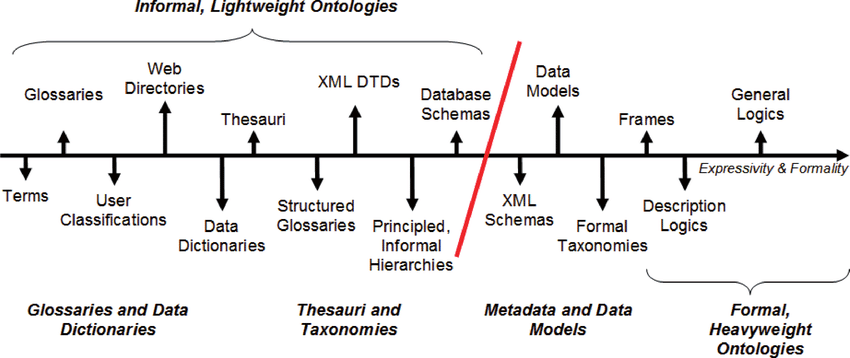
\includegraphics[width=5.51147in,height=2.31944in]{images/media/image19.png}

\emph{Gambar 2.1 Spektrum formalitas ontologi}

Mengacu pada spektrum tersebut, penelitian ini mengadopsi pendekatan
ontologi informal yang berfokus pada pemodelan hierarki taksonomi
konseptual. Pendekatan ini dipilih karena relevansinya dengan realitas
pedagogis saat ini. Berbeda dengan domain lain seperti kesehatan atau
keuangan yang telah banyak mengadopsi ontologi formal, bidang pendidikan
secara historis ditandai oleh ekosistem yang sangat beragam, sehingga
belum memiliki ontologi maupun skema formal yang diterima secara
universal. Oleh karena itu, pendekatan informal yang fleksibel namun
tetap terstruktur secara hierarkis merupakan solusi yang lebih pragmatis
dan sesuai dengan karakteristik domain ini.

\hypertarget{knowledge-graph-completion}{%
\subsubsection{Knowledge Graph
Completion}\label{knowledge-graph-completion}}

Meskipun menawarkan representasi pengetahuan yang lengkap dan
terstruktur, implementasi KG di dunia nyata memiliki keterbatasan
fundamental yaitu sifatnya yang secara inheren tidak lengkap
(\emph{incomplete}). Proses ekstraksi pengetahuan, baik yang dilakukan
secara manual maupun otomatis, hampir selalu gagal menangkap seluruh
fakta yang terkandung dalam sumber teks, sehingga memunculkan fenomena
\emph{missing links} atau relasi yang tidak terpetakan dalam graf. Untuk
mengatasi kekosongan informasi tersebut, dikembangkanlah mekanisme
\emph{Knowledge Graph Completion} (KGC), yakni tugas komputasional yang
bertujuan menginferensi dan memprediksi entitas atau relasi yang hilang
sehingga triple pengetahuan menjadi utuh dan konsisten secara semantik.

Pada fase awal perkembangannya, KGC didominasi oleh metode berbasis
\emph{embedding}, representasi matematis entitas dan relasi dalam ruang
vektor berdimensi rendah, seperti TransE (Bordes et al., 2013)
memodelkan relasi sebagai operasi translasi pada ruang vektor, sehingga
untuk sebuah triple (kepala, relasi, ekor) berlaku pendekatan h + r ≈ t.
Pendekatan ini efisien, namun kesulitan merepresentasikan relasi yang
bersifat simetris maupun satu-ke-banyak . Sebagai penyempurnaan, RotatE
(Sun et al., 2019) memodelkan relasi sebagai rotasi pada ruang kompleks
sehingga mampu menangkap pola relasi yang lebih beragam (simetri,
antisimetri, inversi, dan komposisi), sementara keluarga semantic
matching seperti DistMult (Yang et al., 2015) dan ComplEx (Trouillon et
al., 2016) menilai keabsahan triple melalui kesamaan semantik
antar-vektor. Meskipun berbeda dalam formulasi, seluruh metode ini
memiliki keterbatasan yang sama: kedekatan antarentitas dikalkulasikan
semata-mata berdasarkan struktur topologi graf, tanpa mempertimbangkan
informasi tekstual atau kontekstual yang melingkupinya (Ji et al.,
2022). Keterbatasan inilah yang menjadi semakin menonjol ketika
dihadapkan pada long-tail entities.

Metode-metode ini bekerja dengan mengkalkulasi kedekatan atau jarak
antarentitas semata-mata berdasarkan struktur topologi graf, tanpa
mempertimbangkan informasi tekstual atau kontekstual yang melingkupinya.
Keterbatasan pendekatan ini menjadi semakin menonjol ketika dihadapkan
pada \emph{long-tail entities}, yakni entitas atau sub-topik dengan
tingkat kemunculan yang rendah serta konektivitas relasional yang minim.
Wei et al. (2023) membuktikan secara empiris bahwa metode
\emph{embedding} berbasis triple mengalami degradasi performa yang
signifikan dalam skenario ini, karena representasi vektor entitas yang
jarang terhubung tidak cukup terlatih untuk menghasilkan inferensi yang
valid. Persoalan \emph{long-tail entities} ini memiliki relevansi
langsung terhadap domain pendidikan sains. Distribusi topik dalam
kurikulum sains SMA bersifat asimetris, dimana konsep-konsep lintas
disiplin yang menghubungkan fisika, kimia, dan biologi, misalnya relasi
antara termodinamika dengan metabolisme sel, atau antara ikatan kimia
dengan sifat mekanik material, cenderung jarang tersebut secara
eksplisit dalam satu sumber teks tunggal, sehingga secara struktural
masuk ke dalam kategori \emph{long-tail} dalam graf pengetahuan. Hal ini
berarti metode \emph{embedding} konvensional kurang mampu menemukan dan
melengkapi relasi-relasi interdisipliner yang justru paling bernilai
secara pedagogis.

Untuk mengatasi keterbatasan tersebut, paradigma KGC modern telah
bergeser menuju pendekatan berbasis pemahaman bahasa alami. Yao et al.
(2023) meletakkan landasan teknis yang berpengaruh dengan memperlakukan
triple KG bukan sebagai struktur matematis, melainkan sebagai urutan
teks (\emph{text sequences}). Dengan reformulasi ini, tugas KGC yang
semula berupa perhitungan jarak spasial ditransformasi menjadi tugas
\emph{question answering} berbasis pemahaman semantik, model diminta
menjawab pertanyaan seperti "apa yang berhubungan dengan entitas X
melalui relasi R?" dengan mengandalkan pemahaman konteks bahasa secara
luas. Pendekatan ini membuka jalan bagi integrasi \emph{Large Language
Models} (LLM) ke dalam pipeline KGC, yang menjadi inti kontribusi teknis
penelitian ini dan diuraikan lebih lanjut.

Kapasitas semantik tersebut, di sisi lain, menghadirkan tantangan
komputasional: penerapan LLM secara langsunguntuk mengevaluasi seluruh
kandidat relasi dalam graf berskala besar tidaklah praktis. Pencarian
relasi semantik dengan membandingkan embedding dari seluruh entitas
secara menyeluruh (brute-force) akan menghasilkan kompleksitas waktu
O(n\textsuperscript{2}), yang tidak skalabel untuk graf berskala besar
serta memiliki potensi untuk terhambat oleh \emph{input token limit}
pada arsitektur model bahasa. Oleh karena itu, arsitektur KGC modern
sering kali memanfaatkan teknologi basis data vektor atau algoritma
Approximate Nearest Neighbor (ANN). Pendekatan ini memungkinkan
pencarian kandidat relasi dengan kedekatan semantik tertinggi secara
jauh lebih efisien sebelum dievaluasi lebih lanjut oleh LLM.

\hypertarget{large-language-models-llm-dan-sinergi-llm-kg}{%
\subsubsection{Large Language Models (LLM) dan Sinergi
LLM-KG}\label{large-language-models-llm-dan-sinergi-llm-kg}}

Perkembangan \emph{Large Language Models} (LLM) telah mendorong
pergeseran paradigma dalam ekosistem kecerdasan buatan, khususnya dalam
hubungannya dengan teknologi KG. Pan et al. (2024) memetakan sinergi
antara LLM dan KG ke dalam tiga kerangka konseptual utama:
\emph{KG-enhanced LLMs} (KG digunakan untuk meningkatkan akurasi dan
faktualitas LLM), \emph{LLM-augmented KGs} (LLM dimanfaatkan untuk
menyelesaikan tugas-tugas konstruksi dan penalaran KG), serta
\emph{Synergized LLMs + KGs} (keduanya beroperasi secara resiprokal dan
setara). Penelitian ini secara spesifik beroperasi dalam kerangka
\emph{LLM-augmented KGs}, di mana kapasitas generalisasi semantik LLM
dimanfaatkan untuk menyempurnakan proses konstruksi graf dan
\emph{Knowledge Graph Completion} (KGC), khususnya dalam menangkap
relasi interdisipliner yang tidak tersurat secara eksplisit dalam
kurikulum.

Sinergi ini secara fundamental mengubah arsitektur kerja KGC
tradisional. Bian (2025) mencatat bahwa proses ekstraksi dan konstruksi
KG kini telah bergeser dari pendekatan statistik-simbolik yang
deterministik dan kaku menuju kerangka berbasis model bahasa generatif
yang jauh lebih adaptif dan \emph{context-sensitve}. Pendekatan
deterministik umumnya bergantung pada aturan eksplisit yang ditetapkan
manusia, seperti pencocokan pola sintaksis (regular expression),
rule-based dependency parsing, atau template relasi yang telah
didefinisikan sebelumnya. Sebagai contoh, untuk mengekstraksi relasi
prasyaratDari dari teks materi sains, sistem berbasis aturan harus
dibekali pola eksplisit seperti ``untuk memahami X, siswa perlu
menguasai Y''; akibatnya, ketika struktur kalimat berubah, misalnya
menjadi ``Y merupakan fondasi bagi X'', relasi tersebut dapat gagal
terdeteksi. Kekakuan inilah yang membuat pendekatan deterministik sulit
menangkap relasi implisit dan variasi ekspresi bahasa alami yang
melimpah dalam teks pendidikan.

Keterbatasan tersebut tidak hanya muncul pada tahap ekstraksi, tetapi
juga pada tahap penalaran, karena metode embedding konvensional yang
menggantikan pendekatan berbasis aturan juga memiliki keterbatasan
serupa karena penalarannya hanya bergantung pada pola koneksi yang telah
ada dalam graf, sehingga tetap kesulitan dalam memahami konteks bahasa
yang kaya dan kompleks. Pergeseran menuju penggunaan Large Language
Models (LLM) mendefinisikan ulang mekanisme penalaran dalam Knowledge
Graph Construction (KGC), karena LLM mampu memanfaatkan pengetahuan
internal yang diperoleh dari pelatihan pada korpus teks berskala masif
untuk mengevaluasi kelayakan semantik suatu fakta baru, termasuk pada
entitas long-tail yang memiliki sedikit koneksi dalam graf (Yao et al.,
2023; Wei et al., 2023).

Salah satu implementasi paling representatif dari paradigma ini adalah
kerangka kerja KICGPT (Wei et al., 2023), yang memadukan pipeline KGC
dengan kemampuan penalaran LLM melalui strategi \emph{In-Context
Learning} (ICL). Inti dari strategi ini adalah mekanisme yang disebut
\emph{Knowledge Prompt}: struktur ontologi KG, termasuk entitas, relasi,
dan batasan semantiknya, dikodekan sebagai demonstrasi teks di dalam
instruksi (\emph{prompt}), sehingga LLM memperoleh panduan kontekstual
yang cukup untuk melakukan ranking kandidat relasi tanpa memerlukan
proses \emph{fine-tuning} yang secara komputasional mahal. Pendekatan
ini relevan secara praktis untuk penelitian ini, karena memungkinkan
pemanfaatan LLM dalam skala penelitian akademis tanpa bergantung pada
infrastruktur pelatihan model berskala industri.

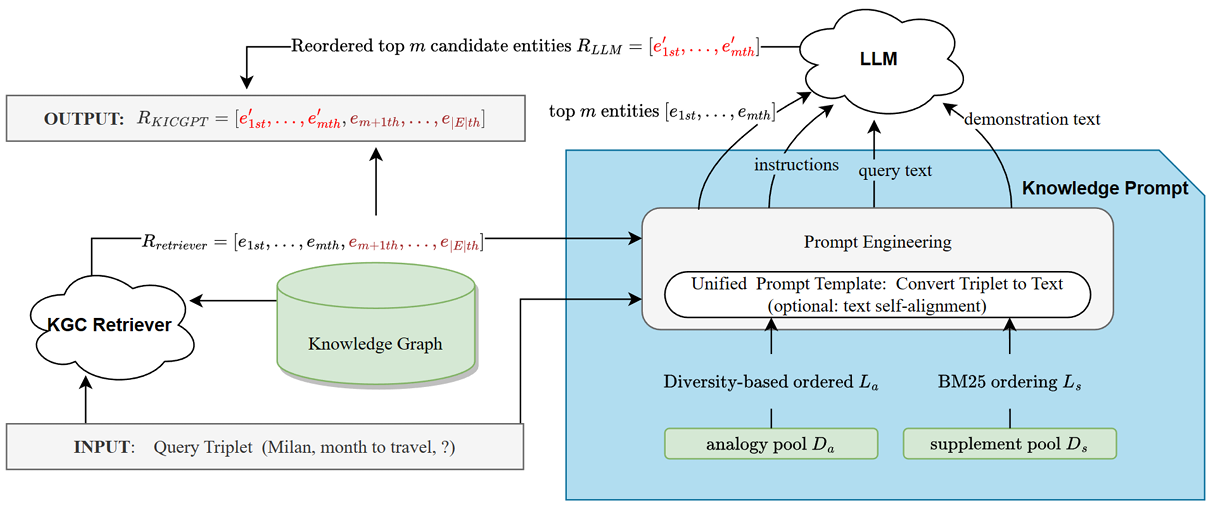
\includegraphics[width=5.51147in,height=2.30556in]{images/media/image15.png}

Gambar X. Ilustrasi kerangka KICGPT

Untuk merangkum pergeseran paradigma yang telah diuraikan di atas, Tabel
2.1 menyajikan perbandingan konseptual antara metode KGC konvensional
berbasis \emph{embedding} dengan pendekatan mutakhir yang dibantu LLM,
mencakup dimensi arsitektur, kemampuan penanganan \emph{long-tail
entities}, kebutuhan data, serta fleksibilitas adaptasi terhadap domain
baru.

\emph{Tabel 2.1 Perbandingan Metode KGC Tradisional dan LLM-Assisted}

\begin{longtable}[]{@{}
  >{\raggedright\arraybackslash}p{(\columnwidth - 4\tabcolsep) * \real{0.1534}}
  >{\raggedright\arraybackslash}p{(\columnwidth - 4\tabcolsep) * \real{0.4242}}
  >{\raggedright\arraybackslash}p{(\columnwidth - 4\tabcolsep) * \real{0.4223}}@{}}
\toprule()
\begin{minipage}[b]{\linewidth}\raggedright
\textbf{Aspek}
\end{minipage} & \begin{minipage}[b]{\linewidth}\raggedright
\textbf{Metode Tradisional (Pre-2021)}
\end{minipage} & \begin{minipage}[b]{\linewidth}\raggedright
\textbf{Metode LLM-Assisted (2021-Sekarang)}
\end{minipage} \\
\begin{minipage}[b]{\linewidth}\raggedright
Data Source
\end{minipage} & \begin{minipage}[b]{\linewidth}\raggedright
Terstruktur (RDF/SQL/Simbolik)
\end{minipage} & \begin{minipage}[b]{\linewidth}\raggedright
Tidak Terstruktur (Buku Teks, Modul, Silabus)
\end{minipage} \\
\begin{minipage}[b]{\linewidth}\raggedright
Context
\end{minipage} & \begin{minipage}[b]{\linewidth}\raggedright
Terbatas pada jarak struktur graf matematis murni
\end{minipage} & \begin{minipage}[b]{\linewidth}\raggedright
Memahami semantik bahasa alami dan konteks teks lintas dokumen
\end{minipage} \\
\begin{minipage}[b]{\linewidth}\raggedright
Scalability
\end{minipage} & \begin{minipage}[b]{\linewidth}\raggedright
Membutuhkan intervensi pakar secara manual secara masif
\end{minipage} & \begin{minipage}[b]{\linewidth}\raggedright
Ekstraksi otomatis dan generatif dengan verifikasi (\emph{In-Context
Learning})
\end{minipage} \\
\begin{minipage}[b]{\linewidth}\raggedright
Long-tail Handling
\end{minipage} & \begin{minipage}[b]{\linewidth}\raggedright
Performa turun drastis pada data minim koneksi
\end{minipage} & \begin{minipage}[b]{\linewidth}\raggedright
Sangat \emph{robust} menambal data memanfaatkan \emph{pre-trained
knowledge} LLM
\end{minipage} \\
\midrule()
\endhead
\bottomrule()
\end{longtable}

\hypertarget{large-language-model-sebagai-penilai-llm-as-a-judge}{%
\subsubsection{\texorpdfstring{2.1.4 \emph{Large Language Model} sebagai
Penilai (LLM-as-a-Judge)
}{2.1.4 Large Language Model sebagai Penilai (LLM-as-a-Judge) }}\label{large-language-model-sebagai-penilai-llm-as-a-judge}}

Dalam KG \emph{Construction}, validasi oleh pakar manusia
(\emph{expert-driven evaluation}) merupakan \emph{gold standard} untuk
memastikan kebenaran faktual berkat kedalaman pemahaman kontekstualnya.
Namun, dalam proses anotasi data, tahapan validasi ini sering kali
memunculkan perbedaan pendapat (\emph{disagreement}) di antara para
pakar akibat tingkat subjektivitas masing-masing penilai (Gu et al.,
2026; Zheng et al., 2023). Untuk mengatasi ketidaksepakatan tersebut
tanpa mengorbankan skalabilitas dan menekan biaya operasional,
pemanfaatan LLM dapat diimplementasikan melalui pendekatan
LLM-as-a-Judge. Dalam skenario ini, alih-alih difungsikan sebagai
penilai utama yang menggantikan peran manusia, LLM diposisikan secara
spesifik sebagai moderator yang objektif untuk menyelesaikan konflik
penilaian antar-pakar (Gu et al., 2026).

Meskipun terbukti efektif sebagai penengah, literatur menunjukkan bahwa
LLM memiliki kerentanan terhadap bias kognitif saat dihadapkan pada dua
argumen yang berseberangan. Model sering kali terpengaruh oleh bias
konkret (\emph{concreteness bias}), di mana LLM cenderung memihak pada
respons yang menyajikan detail spesifik atau dikemas dengan gaya bahasa
yang manipulatif dan meyakinkan, sekalipun argumen tersebut secara
faktual keliru (Gu et al., 2026; Zheng et al., 2023).

Oleh karena itu, untuk menjamin reliabilitas keputusan dan menekan
tingkat halusinasi saat model melakukan arbitrase, proses penengahan
oleh LLM menuntut adanya mekanisme penjangkaran (\emph{grounding}) yang
kuat. Sejalan dengan rekomendasi Gu et al. (2026) dan prinsip evaluasi
presisi faktual dari Min et al. (2023), penerapan LLM-as-a-Judge harus
diiringi dengan injeksi konteks berupa bukti eksternal (\emph{textbook
evidence}). Melalui integrasi referensi buku teks kurikulum, landasan
keputusan tidak lagi bergantung pada asumsi parametrik internal model
yang rentan bias, melainkan berakar pada kebenaran fakta keilmuan yang
disediakan.

\hypertarget{section-2}{%
\subsection{}\label{section-2}}

\hypertarget{metrik-evaluasi-knowledge-graph}{%
\subsection{2.2 Metrik Evaluasi Knowledge
Graph}\label{metrik-evaluasi-knowledge-graph}}

Evaluasi kualitas Knowledge Graph (KG) merupakan aspek krusial dalam
mengukur keberhasilan sistem ekstraksi dan penyelesaian graf yang
dibangun. Xue dan Zou (2022) menegaskan bahwa evaluasi kualitas tidak
hanya bergantung pada karakteristik bawaan data (seperti akurasi,
konsistensi, dan kelengkapan intrinsik), tetapi juga sangat krusial
untuk memastikan kredibilitas graf tersebut saat diimplementasikan pada
aplikasi turunannya\emph{.} Untuk mencapai evaluasi yang komprehensif,
metrik evaluasi KG dapat dikategorikan menjadi tiga kelompok utama:
metrik topologi graf, metrik ekstraksi, dan metrik hubungan
antar-entitas.

\hypertarget{metrik-topologi-graf}{%
\subsubsection{2.2.1 Metrik Topologi Graf}\label{metrik-topologi-graf}}

Evaluasi berbasis topologi graf berfokus pada pengukuran karakteristik
fisik dan distribusi relasi jaringan matematis tanpa memandang makna
semantik dari ontologi. Seo et al. (2022) mengklasifikasikan perhitungan
statistik dasar jaringan seperti kohesi dan kardinalitas ke dalam
kategori metrik graf. Metrik ini sangat krusial untuk memetakan
bagaimana konsep-konsep materi sains berinteraksi satu sama lain secara
struktural. Dalam penelitian ini, analisis topologi graf diukur
menggunakan dua indikator utama:

\hypertarget{average-degree-centrality-adc}{%
\paragraph{Average Degree Centrality
(ADC)}\label{average-degree-centrality-adc}}

\textbf{Average Degree Centrality (ADC)} digunakan untuk mengukur
rata-rata jumlah koneksi yang dimiliki oleh setiap simpul (\emph{node})
dalam graf. Dalam penelitian ini, ADC dihitung dalam dua bentuk, yaitu
ADC graf keseluruhan dan ADC antar-konsep. ADC graf keseluruhan
menghitung seluruh simpul dan relasi yang terdapat dalam basis data
graf, termasuk simpul struktural seperti kelas, bab, subbab, konsep,
serta target konsep. Metrik ini digunakan untuk menggambarkan kepadatan
koneksi pada keseluruhan struktur graf.

\(ADC\  = \frac{1}{|V|}deg(v)\)

Dengan \emph{V} adalah himpunan simpul dalam graf dan deg(v) adalah
jumlah relasi yang terhubung langsung ke simpul \emph{v}.

Selain ADC graf keseluruhan, penelitian ini juga menghitung ADC
antar-konsep, yaitu ADC yang hanya melibatkan simpul konsep dan relasi
langsung antar-konsep. Perhitungan ini digunakan untuk merepresentasikan
tingkat keterhubungan konseptual antar-materi sains tanpa dipengaruhi
oleh simpul struktural.

Dengan demikian, ADC graf keseluruhan merepresentasikan kepadatan
koneksi struktur Knowledge Graph secara menyeluruh, sedangkan ADC
antar-konsep merepresentasikan tingkat keterhubungan langsung
antar-konsep materi sains. Dalam konteks penelitian ini, ADC
antar-konsep digunakan sebagai metrik utama untuk membandingkan graf
sebelum dan sesudah proses Knowledge Graph Completion, karena metrik
tersebut lebih langsung mencerminkan perubahan interkoneksi materi
Fisika, Kimia, dan Biologi.

\hypertarget{modularity}{%
\paragraph{Modularity}\label{modularity}}

\textbf{Modularity} (��) mengukur seberapa baik sebuah graf terbagi
menjadi komunitas-komunitas yang terpisah. Nilai modularity berkisar
antara \(- 0,5\) hingga \(1\), nilai yang lebih tinggi menunjukkan
pembagian komunitas yang lebih baik, ditandai dengan koneksi yang rapat
di dalam komunitas dan jarang di luar komunitas. Nilai Q = 0 menunjukkan
bahwa pembagian komunitas yang dihasilkan tidak lebih baik dari partisi
acak.

Modularity dihitung dengan membandingkan dua hal: jumlah \emph{edge}
yang benar-benar ada dalam komunitas, dan jumlah \emph{edge} yang secara
statisktik diharapkan muncul apabila koneksi antar simpul disebar secara
acak, dengan syarat distribusi \emph{degree} tiap tiap simpul
dipertahankan. Selisih antara keduanya menentukan apakah suatu komunitas
lebih padat dari yang diharapkan secara kebetulan.

Untuk graf berarah (\emph{directed graph}), modularity didefinisikan
sebagai:

\(Q = \frac{1}{m}\left\lbrack A_{ij} - \frac{k_{i}^{out}k_{j}^{in}}{m}\delta\left( c_{i}c_{j} \right) \right\rbrack\)

Dengan:

\href{http://www.texrendr.com/?eqn=A_\%7Bij\%7D\#0}{\includegraphics[width=0.23611in,height=0.13889in]{images/media/image6.gif}}:
Matriks adjasensi, bernilai 1 jika terdapat \emph{edge} dari \emph{node}
i ke \emph{node} j, dan 0 jika tidak ada.

\(k_{i}^{out}\): Out-degree dari node i (jumlah edge yang keluar dari
node i).

\(k_{j}^{in}\): In-degree dari ndoe j (jumlah edge yang masuk ke node
j).

\href{http://www.texrendr.com/?eqn=m\#0}{\includegraphics[width=0.15278in,height=\textheight]{images/media/image1.gif}}:
total jumlah \emph{edge} berarah

\(\delta\left( c_{i}c_{j} \right) = 1\): jika simpul
\href{http://www.texrendr.com/?eqn=i\#0}{\includegraphics[width=\textwidth,height=0.11111in]{images/media/image10.gif}}
dan
\href{http://www.texrendr.com/?eqn=j\#0}{\includegraphics[width=\textwidth,height=0.13889in]{images/media/image17.gif}}
berada dalam komunitas yang sama

Rumus di atas dapat diekspresikan dalam bentuk yang lebih ringkas dengan
menjumlahkan langsung per komunitas:

\(Q = \left\lbrack \frac{e_{cc}^{}}{m} - \frac{k_{c}^{out}k_{c}^{in}}{m^{2}} \right\rbrack\)

dengan \hspace{0pt}\(e_{cc}^{}\) adalah jumlah edge internal komunitas
\(c\), sementara \(k_{c}^{out}\) \hspace{0pt} dan \(k_{c}^{in}\)adalah
total out-degree dan in-degree seluruh node dalam komunitas \(c\). Kedua
bentuk rumus ini menghasilkan nilai yang identik, perbedaannya hanya
pada cara penjumlahan, yaitu per pasangan node pada formula pertama,
atau per komunitas pada formula kedua.

\begin{enumerate}
\def\labelenumi{\Alph{enumi}.}
\setcounter{enumi}{2}
\item
  \textbf{Density}
\end{enumerate}

\textbf{Graph Density (D)} mengukur seberapa banyak koneksi yang
terbentuk dalam sebuah graf dibandingkan dengan koneksi maksimum yang
secara teoritis mungkin ada. Nilai D berkisar antara 0 hingga 1, nilai
mendekati 1 menandakan graf yang sangat padat (\emph{dense}), sementara
nilai mendekati 0 menandakan graf yang jarang (\emph{sparse}). Dalam
konteks KG, \emph{density} digunakan untuk membandingkan tingkat
keterkaitan antar konsep sebelum dan sesudah penambahan relasi lintas
buku (\emph{cross-book links}). Peningkatan nilai D setelah penambahan
\emph{cross-book links} mengindikasikan bahwa koneksi antar entitas dari
mata pelajaran yang berbeda berhasil memperkaya struktur graf secara
keseluruhan. Untuk graf berarah (directed graph), formula yang digunakan
adalah:

\(D\  = \ \frac{|E|}{|V|(|V| - 1)}\)

Dengan:

\(|E|\): Jumlah total \emph{edge} yang terbentuk dalam KG.

\(|V|\): Jumlah total \emph{node}.

\(|V|(|V| - 1)\): Jumlah maksimum \emph{edge} berarah yang mungkin ada,
diperoleh dari asumsi bahwa setiap pasangan \emph{node}
\((i,\ j)\ \)dengan \(i\  \neq \ j\) dapat memiliki tepat satu
\emph{edge} berarah tanpa memperbolehkan \emph{self-loop}.

\hypertarget{metrik-ekstraksi}{%
\subsubsection{2.2.2 Metrik Ekstraksi}\label{metrik-ekstraksi}}

Metrik ekstraksi mengevaluasi kualitas proses ekstraksi entitas dan
atribut dari dokumen sumber.

\begin{enumerate}
\def\labelenumi{\alph{enumi}.}
\item
  Description Completeness
\end{enumerate}

\textbf{Description Completeness} mengukur sejauh mana entitas yang
berhasil diidentifikasi juga memiliki informasi pendukung berupa
deskripsi atau definisi. Dalam konteks materi sains, sebuah entitas
seperti "Fotosintesis" atau "Hukum Ohm" tidak cukup hanya muncul sebagai
nama, ia harus memiliki deskripsi agar dapat digunakan dalam proses
pembelajaran atau Knowledge Graph Completion. Pada penelitian ini, DC
didefinisikan sebagai proporsi entitas yang memiliki deskripsi tidak
kosong terhadap seluruh entitas yang diekstraksi:

\(DC\  = \ \frac{|\{\ v\  \in \ V:\ desc(v)\  \neq \ \varnothing\}|}{|V|}\)

dengan

\(V\): Himpunan seluruh entitas yang diekstraksi mencakup node bertipe
\emph{:Concept} (menggunakan atribut \emph{description}) dan
\emph{:Chapter} (menggunakan atribut \emph{summary})

\(\{\ v\  \in \ V:\ desc(v)\  \neq \ \varnothing\}\): Himpunan entitas
yang memiliki deskripsi tidak kosong

\(|V|\): Jumlah total entitas yang diekstraksi. Target minimal untuk
metrik ini ditetapkan sebesar ≥ 0,90 (90\%).

\begin{enumerate}
\def\labelenumi{\alph{enumi}.}
\setcounter{enumi}{1}
\item
  Empty SubKonsep Rate
\end{enumerate}

\textbf{Empty SubKonsep Rate (ESR)} digunakan untuk mengevaluasi
efektivitas dekomposisi struktural dalam Knowledge Graph. Ontologi yang
dikembangkan menerapkan hierarki ketat dari \emph{:Chapter} ke
\emph{:Subtopic} hingga ke unit terkecil yaitu \emph{:Concept}. Dalam
hierarki ini, setiap entitas pada tingkat induk (\emph{parent}) induk
seharusnya memiliki setidaknya satu entitas turunan sebagai hasil
dekomposisi materi. ESR mengukur proporsi entitas induk yang tidak
memiliki satu pun entitas turunan (\emph{child}), yang mengindikasikan
adanya kegagalan dalam proses dekomposisi materi oleh LLM.

\(ESR\  = \ \frac{|\{ k\ \epsilon\ K\ :\ |SK(k)\  = \ 0\ |\}}{|K|}\)

Dengan:

\(K\): Himpunan seluruh entitas pada level hierarki induk (misalnya
\emph{:Subtopic}).

\(|SK(k)|\): Jumlah entitas turunan (misalnya \emph{:Concept}) dari
entitas \(k\) yang terhubung melalui relasi hierarkis :HAS\_CONCEPT.

\(|K|\): Total entitas induk yang diekstraksi. Pembilang menghitung
entitas induk yang tidak memiliki satu pun turunan (\emph{empty
subtopic}).

Metrik ini merujuk pada prinsip \emph{Class Instantiation} yang
dikemukakan oleh Seo et al., di mana setiap kelas yang didefinisikan
dalam ontologi harus dimanfaatkan secara aktif untuk menampung data.
Dalam konteks kurikulum sains, nilai ESR yang rendah menjamin bahwa
setiap topik besar telah berhasil dipecah menjadi konsep-konsep
operasional, sehingga menghindari adanya "node buntu" yang tidak
informatif dalam peta pembelajaran. Target maksimal untuk metrik ini
ditetapkan sebesar \(\leq 0,10\) (10\%).

\begin{enumerate}
\def\labelenumi{\alph{enumi}.}
\setcounter{enumi}{2}
\item
  Typed Relation Ratio
\end{enumerate}

\textbf{Typed Relation Ratio (TRR)} mengukur sejauh mana LLM mampu
mengklasifikasikan hubungan antar-materi ke dalam kategori relasi
semantik yang didefiniskan dalam ontologi dibandingkan dengan penggunaan
relasi generik. Berdasarkan ontologi yang didefinisikan, terdapat 20
tipe relasi spesifik yang terbagi menjadi dua kelompok: intra-buku (15
tipe, seperti :MENYEBABKAN atau :PRASYARAT\_UNTUK) dan lintas-buku (5
tipe, seperti :LINTAS\_BUKU\_APLIKASI\_DARI).

\href{https://www.codecogs.com/eqnedit.php?latex=TRR\%20\%3D\%20\%5Cfrac\%7B\%7CT_\%7Btyped\%7D\%7C\%7D\%7B\%7CT_\%7Btotal\%7D\%7C\%7D\#0}{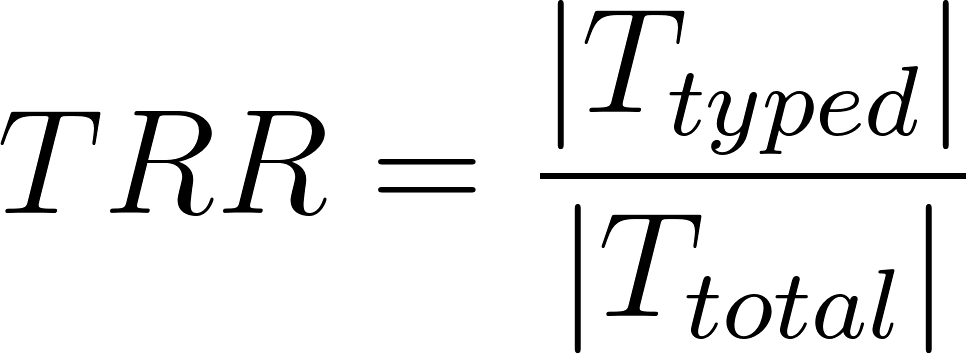
\includegraphics[width=1.09722in,height=0.40278in]{images/media/image12.png}}

Keterangan:

T\textsubscript{typed} : Himpunan relasi di dalam graf yang menggunakan
tipe relasi spesifik (sesuai \emph{controlled vocabulary} dari
ontologi).

\textbar T\textsubscript{typed}\textbar{} : Jumlah total relasi yang
didefinisikan dalam ontologi.

\textbar T\textsubscript{total}\textbar{} : Jumlah keseluruhan relasi
yang ada di dalam KG.

Nilai TRR yang tinggi menunjukkan bahwa setiap relasi dalam KG tidak
hanya menghubungkan dua konsep, tetapi juga dilengkapi dengan anotasi
tekstual yang menjelaskan alasan di balik terbentuknya hubungan
tersebut. Anotasi ini penting karena membedakan KG yang bersifat
\emph{assertional} (sekadar menyatakan bahwa dua entitas berhubungan)
dari KG yang bersifat \emph{explanatory} (yang mampu menjelaskan mengapa
hubungan itu ada). Dengan klasifikasi relasi yang eksplisit dan
deskriptif, sistem dapat melakukan analisis jalur pembelajaran
lintas-buku secara lebih akurat dan bermakna.

\hypertarget{validasi-manusia-human-evaluation}{%
\subsubsection{\texorpdfstring{2.2.4 Validasi Manusia (\emph{Human
Evaluation})}{2.2.4 Validasi Manusia (Human Evaluation)}}\label{validasi-manusia-human-evaluation}}

Selain mengandalkan metrik kuantitatif, proses evaluasi Knowledge Graph
(KG) mutlak membutuhkan validasi kualitatif oleh pakar terkait. Hal ini
krusial mengingat proses KGC dalam penelitian ini dibantu oleh LLM yang
rentan terhadap halusinasi informasi, seperti mengekstrak entitas yang
salah atau memetakan relasi lintas disiplin yang tidak relevan secara
pedagogis. Dalam evaluasi klasifikasi tradisional, prediksi sistem
dinilai secara biner, hanya ada benar (1.0) atau salah (0.0), yang
disebut sebagai himpunan tegas (\emph{crisp sets}). Namun, dalam
evaluasi ekstraksi pengetahuan oleh LLM, hasil sering kali memiliki
batas yang tidak tegas (\emph{soft boundaries}) karena adanya nilai
kebenaran parsial (Harju \& Mesaros, 2023).

Untuk mengakomodasi hal tersebut, penelitian ini mengadopsi metrik Fuzzy
Precision and Recall. Berdasarkan teori himpunan fuzzy, setiap elemen
memiliki nilai keanggotaan (\emph{membership value}) antara 0 hingga 1
yang merepresentasikan derajat kebenarannya (Harju \& Mesaros, 2023).
Dalam penelitian ini, kategori evaluasi pakar dipetakan ke dalam nilai
keanggotaan fuzzy sebagai berikut:

\begin{itemize}
\item
  \textbf{Benar (1.0)}: Representasi keanggotaan penuh (\emph{full
  membership}), di mana relasi 100\% akurat secara keilmuan.
\item
  \textbf{Sebagian Benar (0.5)}: Representasi keanggotaan parsial, di
  mana relasi mengandung fakta saintifik namun memerlukan perbaikan
  deskripsi, sehingga mempertahankan setengah dari nila.
\item
  \textbf{Kurang Konteks (0.25)}: Representasi derajat keanggotaan yang
  lebih lemah. Informasi teknis ada, namun ketiadaan konteks membatasi
  fungsionalitas relasi tersebut dalam graf pembelajaran.
\item
  \textbf{Salah / Triple Hilang (0.0)}: Representasi nol keanggotaan, di
  mana relasi keliru secara ontologis atau gagal diekstraksi.
\end{itemize}

Untuk menghitung metrik evaluasi ini, Harju \& Mesaros (2023)
menggunakan prinsip irisan fuzzy (\emph{fuzzy intersection}) yang
didefinisikan sebagai nilai minimum antara prediksi model dan referensi
ground truth pakar, yaitu \(\ min(ŷ_{i},y)\). Karena model LLM selalu
menghasilkan prediksi dengan tingkat keyakinan penuh \((ŷ_{i} = 1.0)\),
nilai irisan dari setiap relasi akan selalu mengikuti skor keanggotaan
yang ditetapkan oleh pakar. Penjumlahan dari nilai irisan minimum ini
bertindak sebagai pembilang dalam metrik pengukuran. Dengan demikian,
rumus evaluasi \emph{Fuzzy Precision}, \emph{Fuzzy Recall}, dan
\emph{F1-Score} dirumuskan secara operasional sebagai berikut:

\begin{enumerate}
\def\labelenumi{\arabic{enumi}.}
\item
  \textbf{Fuzzy Precision:} Mengukur tingkat akurasi dari keseluruhan
  relasi yang berhasil diekstrak oleh model LLM.
\end{enumerate}

\(Precision\  = \frac{Benar\  + \ (Sebagian\ Benar\  \times \ 0,5) + (0.25 \times KurangKonteks)\ }{Benar + SebagianBenar + KurangKonteks + Salah}\)

\begin{enumerate}
\def\labelenumi{\arabic{enumi}.}
\setcounter{enumi}{1}
\item
  \textbf{Fuzzy Recall:} Mengukur sejauh mana sistem berhasil menangkap
  seluruh relasi penting yang diwajibkan dalam kurikulum, di mana
  penyebut merepresentasikan kardinalitas total dari himpunan referensi
  pakar, termasuk relasi yang gagal diekstraksi (Hilang).
\end{enumerate}

\(Recall\  = \frac{Benar\  + \ (Sebagian\ Benar\  \times \ 0,5) + (0.25 \times KurangKonteks)\ }{Benar + SebagianBenar + KurangKonteks + Hilang}\)

\begin{enumerate}
\def\labelenumi{\arabic{enumi}.}
\setcounter{enumi}{2}
\item
  \textbf{F1-Score:} Rata-rata harmonik antara Precision dan Recall
  untuk memberikan representasi kualitas ekstraksi model secara
  keseluruhan.
\end{enumerate}

\(F1\ Score\  = 2\  \times \frac{Precision\  \times \ Recall}{Precision\  + \ Recall}\)

Melalui pendekatan ini, evaluasi kualitatif dari pakar secara langsung
diterjemahkan menjadi indikator performa kuantitatif, sehingga kualitas
dan kelayakan Knowledge Graph untuk diimplementasikan dalam Kurikulum
Merdeka dapat dipertanggungjawabkan secara komputasional maupun
pedagogis.

\textbf{Pengujian Reliabilitas Pakar (Inter-rater Reliability)}

Untuk memastikan bahwa penentuan validitas suatu relasi sains tidak
didasari oleh bias subjektif individu, evaluasi kualitatif harus
diiringi dengan perhitungan tingkat kesepakatan antar-penilai
(\emph{inter-rater agreemen}t).

Pada evaluasi sistem LLM, khususnya ketika \emph{output} sistem
diprediksi memiliki akurasi tinggi, distribusi label yang diberikan oleh
pakar cenderung tidak seimbang (\emph{imbalanced}), yaitu ketika satu
kategori (misalnya label "Benar") muncul jauh lebih dominan dibandingkan
kategori lainnya. Pada kondisi distribusi yang miring (\emph{skewed})
seperti ini, metrik konvensional seperti \emph{Cohen\textquotesingle s
Kappa} kurang cocok karena rentan terhadap Kappa Paradox, fenomena
ketika Kappa cenderung meremehkan tingkat kesepakatan pada skenario yang
sangat tidak seimbang, sehingga menghasilkan skor rendah meskipun
kesepakatan aktual antar-pakar sangat tinggi (James, 2026).

\(AC1 = \frac{P_{a} - \ P_{e}}{1\  - \ P_{e}}\)

Dengan \(P_{a}\)\hspace{0pt} adalah proporsi kesepakatan aktual
(\emph{observed agreement}) antar-pakar, dan
\(P_{e}\)\hspace{0pt}\hspace{0pt} proporsi kesepakatan yang diharapkan
terjadi secara kebetulan (\emph{expected agreement}),yang dirumuskan
sebagai:

\(P_{e} = \frac{1}{q - 1}{p\hat{}}_{k}(1 - {p\hat{}}_{k})\)

dengan \(q\) adalah jumlah kategori label dan \({p\hat{}}_{k}\) adalah
proporsi penilai yang menetapkan label kategori \(k\). Rumus
\(P_{e}\)\hspace{0pt} inilah yang membedakan Gwet\textquotesingle s AC1
dari Kappa, estimasi peluang kesepakatan dihitung berdasarkan proporsi
penggunaan kategori secara aktual, sehingga nilai AC1 tetap mencerminkan
kesepakatan yang sesungguhnya meskipun satu label muncul jauh lebih
sering daripada label lainnya. (Mahbub et al., 2025)

Nilai AC1 berada pada rentang −1 hingga 1, nilai yang lebih tinggi
mencerminkan kesepakatan yang lebih kuat di luar kebetulan, dengan
kategori interpretatif sebagai berikut: buruk (\textless0,40), sedang
(0,40--0,60), baik (0,60--0,80), dan sangat baik (\textgreater0,80).

\hypertarget{interkoneksi-materi-sains-dalam-konteks-kurikulum-merdeka}{%
\subsection{2.3 Interkoneksi Materi Sains dalam Konteks Kurikulum
Merdeka}\label{interkoneksi-materi-sains-dalam-konteks-kurikulum-merdeka}}

Penerapan rekayasa pengetahuan komputasional dalam penelitian ini
difokuskan pada domain pendidikan menengah khususnya kelas 12 di
Indonesia, yang saat ini berpedoman pada Kurikulum Merdeka. Kurikulum
ini dirancang untuk mendorong \emph{meaningful learning} (pembelajaran
bermakna) dan penguasaan kompetensi pemecahan masalah lintas disiplin,
sebuah orientasi yang secara filosofis sejalan dengan argumen Abdel-Radi
(2025), bahwa tantangan global abad ke-21 tidak dapat lagi diselesaikan
dari satu sudut pandang spesialisasi tunggal, melainkan menuntut
"kesatuan pengetahuan" (\emph{unity of knowledge}) yang bersifat
interdisipliner. Dengan demikian, semangat integrasi lintas disiplin
bukan sekadar aspirasi pedagogis, melainkan respons terhadap tuntutan
kompetensi yang nyata.

Namun, di level implementasi, terdapat kesenjangan struktural yang
signifikan antara filosofi kurikulum dan realitas pembelajaran di kelas.
Pada jenjang SMA Fase F, rumpun mata pelajaran Ilmu Pengetahuan Alam
(IPA) tetap diajarkan sebagai tiga mata pelajaran yang terpisah secara
administratif: Fisika, Kimia, dan Biologi. Pemisahan ini melahirkan
fenomena \emph{siloed learning}, kondisi di mana batas-batas disipliner
yang kaku menghalangi peserta didik untuk mengkonstruksi koneksi
konseptual antar mata pelajaran. Wuli et al. (2025) mencatat bahwa dalam
kondisi ini, siswa kesulitan mengaitkan konsep yang secara ontologis
berkaitan, sementara guru menghadapi kebingungan metodologis dalam
merancang pembelajaran yang terintegrasi karena minimnya referensi
kurikulum lintas mata pelajaran yang tersedia secara terstruktur.

Kesenjangan ini secara tidak langsung juga merupakan masalah
representasi pengetahuan: relasi-relasi interdisipliner yang ada dalam
sains tidak pernah dikodifikasi secara eksplisit dalam dokumen
kurikulum. Sebagai respons pedagogis, pendekatan pemetaan
\emph{Disciplinary Core Ideas} (DCI) dan \emph{Interdisciplinary Core
Ideas} (ICI) telah terbukti menjanjikan. Semilarski et al. (2022)
membuktikan bahwa pemetaan visual konsep inti lintas disiplin sains
secara signifikan meningkatkan efikasi diri (\emph{self-efficacy})
siswa. Namun, studi yang sama juga mengidentifikasi hambatan penting:
guru dan siswa mengalami kesulitan ketika harus memetakan irisan
konsep-konsep abstrak, terutama antara Fisika dan Kimia, secara manual,
mengindikasikan bahwa pendekatan ini memerlukan dukungan komputasional
agar dapat berjalan secara efisien.

Kebutuhan akan otomatisasi inilah yang menjadi justifikasi metodologis
inti penelitian ini. Acuan serupa telah diletakkan oleh Said et al.
(2024), yang mengekstraksi kata kunci esensial dari silabus sains dan
matematika untuk memetakan interkoneksinya terhadap Tujuan Pembangunan
Berkelanjutan (SDGs) secara komputasional. Penelitian ini mengadopsi dan
memperluas logika serupa dengan memanfaatkan metode \emph{LLM-Assisted
Knowledge Graph Completion}: konsep-konsep materi sains yang tersebar
dan terisolasi secara struktural diorganisasi ke dalam KG, kemudian LLM
ditugaskan untuk menginferensi relasi interdisipliner yang bersifat
implisit di antara konsep-konsep Fisika, Kimia, dan Biologi.

\hypertarget{metodologi-penelitian}{%
\section{\texorpdfstring{\hfill\break
METODOLOGI
PENELITIAN}{ METODOLOGI PENELITIAN}}\label{metodologi-penelitian}}

Untuk mencapai tujuan penelitian, diperlukan kerangka kerja yang jelas
dalam membangun dan menguji sistem \emph{Knowledge Graph Completion
berbasis Large Language Model}. Penelitian ini dirancang dengan tahapan
yang sistematis, mulai dari pengumpulan data kurikulum, pengembangan
sistem, hingga evaluasi oleh pakar untuk memastikan hasil yang
dihasilkan akurat dan bermanfaat.

\hypertarget{desain-penelitian}{%
\subsection{Desain Penelitian}\label{desain-penelitian}}

Penelitian ini menggunakan pendekatan \emph{Design Science Research}
(DSR) dengan fokus pada pengembangan purwarupa sistem Knowledge Graph
Completion berbasis Large Language Model (LLM). Pendekatan DSR dipilih
karena penelitian ini secara spesifik bertujuan untuk menghasilkan
solusi berupa artefak inovatif yang dapat memecahkan masalah, yakni
fragmentasi pemahaman lintas disiplin pada kurikulum sains jenjang SMA

Menurut Hevner et al. (2004), DSR adalah paradigma pemecahan masalah
yang berupaya meningkatkan batasan kapabilitas manusia dan organisasi
dengan menciptakan artefak baru yang inovatif, yang direpresentasikan
dalam bentuk konstruk (constructs), model (models), metode (methods),
dan instansiasi (instantiations). Dalam konteks penelitian ini, desain
artefak yang dikembangkan mencakup:

\begin{enumerate}
\def\labelenumi{\arabic{enumi}.}
\item
  \textbf{Instansiasi (Purwarupa Sistem):} Dashboard interaktif berbasis
  Neo4j untuk menyimpan, menelusuri, dan memvisualisasikan Knowledge
  Graph kurikulum sains secara terintegrasi.
\item
  \textbf{Metode (Algoritma dan Pipeline):} Algoritma ekstraksi
  pengetahuan terstruktur menggunakan LLM dengan output berbasis
  ontologi, serta pipeline KG Construction dan Completion yang akan
  dijelaskan di subbab 3.5.
\end{enumerate}

Secara metodologis, penelitian ini dikategorikan sebagai penelitian
terapan (\emph{applied research}) yang diuraikan pada tabel berikut:

\begin{longtable}[]{@{}
  >{\raggedright\arraybackslash}p{(\columnwidth - 2\tabcolsep) * \real{0.5000}}
  >{\raggedright\arraybackslash}p{(\columnwidth - 2\tabcolsep) * \real{0.5000}}@{}}
\toprule()
\begin{minipage}[b]{\linewidth}\raggedright
\textbf{Karakteristik}
\end{minipage} & \begin{minipage}[b]{\linewidth}\raggedright
\textbf{Deskripsi}
\end{minipage} \\
\begin{minipage}[b]{\linewidth}\raggedright
Jenis Penelitian
\end{minipage} & \begin{minipage}[b]{\linewidth}\raggedright
Terapan (\emph{Applied Research})
\end{minipage} \\
\begin{minipage}[b]{\linewidth}\raggedright
Pendekatan
\end{minipage} & \begin{minipage}[b]{\linewidth}\raggedright
Design Science Research (DSR)
\end{minipage} \\
\begin{minipage}[b]{\linewidth}\raggedright
Metode
\end{minipage} & \begin{minipage}[b]{\linewidth}\raggedright
Eksperimental dengan validasi kualitatif pakar
\end{minipage} \\
\begin{minipage}[b]{\linewidth}\raggedright
Output
\end{minipage} & \begin{minipage}[b]{\linewidth}\raggedright
Artefak sistem (Metode KGC dan Purwarupa Visualisasi)
\end{minipage} \\
\begin{minipage}[b]{\linewidth}\raggedright
Paradigma
\end{minipage} & \begin{minipage}[b]{\linewidth}\raggedright
Pragmatisme (Berfokus pada utilitas dan pemecahan masalah)
\end{minipage} \\
\midrule()
\endhead
\bottomrule()
\end{longtable}

Adopsi DSR dalam penelitian ini mengikuti kerangka kerja yang diusulkan
oleh Peffers et al. (2007), meliputi enam tahapan:

\begin{enumerate}
\def\labelenumi{\arabic{enumi}.}
\item
  \textbf{Identifikasi Masalah} --- Fragmentasi kurikulum sains lintas
  disiplin (Fisika, Kimia, Biologi) menyebabkan siswa kesulitan melihat
  keterhubungan konsep
\item
  \textbf{Definisi Tujuan} --- Mengembangkan sistem yang dapat menemukan
  relasi implisit antar-konsep lintas mata pelajaran
\item
  \textbf{Desain dan Pengembangan} --- Membangun \emph{pipeline}
  ekstraksi-konstruksi-penyempurnaan \emph{knowledge graph}
\item
  \textbf{Demonstrasi} --- Menerapkan artefak yang telah dibangun untuk
  memecahkan masalah dengan memproses Buku Teks Resmi Kemendikbudristek
\item
  \textbf{Evaluasi} --- Pengukuran metrik struktural (ADC, Modularity),
  metrik ekstraksi, dan validasi pakar
\item
  \textbf{Komunikasi} --- Dokumentasi dalam bentuk skripsi dan publikasi
  ilmiah

  \begin{enumerate}
  \def\labelenumii{\arabic{enumii}.}
  \item ~
    \hypertarget{lokasi-dan-waktu-penelitian}{%
    \subsection{Lokasi dan Waktu
    Penelitian}\label{lokasi-dan-waktu-penelitian}}

    \begin{enumerate}
    \def\labelenumiii{\arabic{enumiii}.}
    \item ~
      \hypertarget{lokasi-penelitian}{%
      \subsubsection{Lokasi Penelitian}\label{lokasi-penelitian}}
    \end{enumerate}
  \end{enumerate}
\end{enumerate}

Penelitian ini dilaksanakan secara \emph{online} tanpa melibatkan studi
lapangan.

\hypertarget{waktu-penelitian}{%
\subsubsection{Waktu Penelitian}\label{waktu-penelitian}}

Penelitian direncanakan berlangsung selama 6 (enam) bulan, dimulai dari
Januari 2026 hingga Juni 2026. Rincian tahapan waktu penelitian
disajikan pada tabel berikut:

\begin{longtable}[]{@{}
  >{\raggedright\arraybackslash}p{(\columnwidth - 4\tabcolsep) * \real{0.1061}}
  >{\raggedright\arraybackslash}p{(\columnwidth - 4\tabcolsep) * \real{0.5606}}
  >{\raggedright\arraybackslash}p{(\columnwidth - 4\tabcolsep) * \real{0.3333}}@{}}
\toprule()
\begin{minipage}[b]{\linewidth}\raggedright
\textbf{Fase}
\end{minipage} & \begin{minipage}[b]{\linewidth}\raggedright
\textbf{Kegiatan}
\end{minipage} & \begin{minipage}[b]{\linewidth}\raggedright
\textbf{Periode}
\end{minipage} \\
\begin{minipage}[b]{\linewidth}\raggedright
1
\end{minipage} & \begin{minipage}[b]{\linewidth}\raggedright
Studi literatur dan desain sistem
\end{minipage} & \begin{minipage}[b]{\linewidth}\raggedright
Januari - Februari 2026
\end{minipage} \\
\begin{minipage}[b]{\linewidth}\raggedright
2
\end{minipage} & \begin{minipage}[b]{\linewidth}\raggedright
Implementasi pipeline ekstraksi
\end{minipage} & \begin{minipage}[b]{\linewidth}\raggedright
Februari - Maret 2026
\end{minipage} \\
\begin{minipage}[b]{\linewidth}\raggedright
3
\end{minipage} & \begin{minipage}[b]{\linewidth}\raggedright
Konstruksi \emph{Knowledge Graph}
\end{minipage} &
\multirow{2}{*}{\begin{minipage}[b]{\linewidth}\raggedright
Maret - April 2026
\end{minipage}} \\
\begin{minipage}[b]{\linewidth}\raggedright
4
\end{minipage} & \begin{minipage}[b]{\linewidth}\raggedright
Evaluasi dan validasi pakar \#1
\end{minipage} \\
\begin{minipage}[b]{\linewidth}\raggedright
5
\end{minipage} & \begin{minipage}[b]{\linewidth}\raggedright
\emph{Knowledge Graph Completion}
\end{minipage} & \begin{minipage}[b]{\linewidth}\raggedright
April 2026
\end{minipage} \\
\begin{minipage}[b]{\linewidth}\raggedright
6
\end{minipage} & \begin{minipage}[b]{\linewidth}\raggedright
Evaluasi dan validasi pakar \#2
\end{minipage} & \begin{minipage}[b]{\linewidth}\raggedright
Mei 2026
\end{minipage} \\
\begin{minipage}[b]{\linewidth}\raggedright
7
\end{minipage} & \begin{minipage}[b]{\linewidth}\raggedright
Analisis hasil dan penulisan
\end{minipage} & \begin{minipage}[b]{\linewidth}\raggedright
Mei - Juni 2026
\end{minipage} \\
\midrule()
\endhead
\bottomrule()
\end{longtable}

\hypertarget{sumber-data-dan-korpus-penelitian}{%
\subsection{Sumber Data dan Korpus
Penelitian}\label{sumber-data-dan-korpus-penelitian}}

Dalam pengembangan sistem ekstraksi dan Knowledge Graph Completion
(KGC), penelitian ini tidak menggunakan populasi manusia sebagai objek
eksperimen utama, melainkan menggunakan dua jenis data yang saling
melengkapi, yaitu data tekstual sebagai korpus ekstraksi dan data
penilaian pakar sebagai dasar evaluasi model.

\hypertarget{section-3}{%
\subsubsection{\texorpdfstring{\hfill\break
}{ }}\label{section-3}}

\hypertarget{data-primer-korpus-ekstraksi}{%
\subsubsection{\texorpdfstring{\textbf{3.3.1} Data Primer (Korpus
Ekstraksi)
}{3.3.1 Data Primer (Korpus Ekstraksi) }}\label{data-primer-korpus-ekstraksi}}

Data primer yang digunakan sebagai sumber ekstraksi pengetahuan dibatasi
pada materi sains tingkat SMA Fase F (Kelas XII). Teknik pengambilan
sampel dokumen dilakukan secara \emph{purposive sampling} berdasarkan
relevansinya dengan Kurikulum Merdeka. Korpus penelitian ini terdiri
dari buku teks siswa (\emph{e-book)} terbitan Kemendikbudristek untuk
mata pelajaran Fisika, Kimia, dan Biologi Fase F (Kelas XII). Pembatasan
korpus pada buku teks resmi ini bertujuan untuk memastikan bahwa entitas
materi dan relasi dasar yang diekstrak oleh sistem pada tahap awal
(\emph{initial graph}) benar-benar mencerminkan standar ontologi materi
yang diajarkan secara nasional.

\hypertarget{data-validasi-pakar-expert-validation-data}{%
\subsubsection{\texorpdfstring{3.3.2 Data Validasi Pakar (Expert
Validation Data)
}{3.3.2 Data Validasi Pakar (Expert Validation Data) }}\label{data-validasi-pakar-expert-validation-data}}

Data validasi diperoleh melalui penilaian kualitatif oleh panel pakar
(\emph{expert validation}) terhadap triple relasi, khususnya
interkoneksi lintas disiplin, yang dihasilkan oleh sistem KGC berbasis
LLM. Pengumpulan data ini dilakukan melalui aplikasi web KG Review App,
di mana setiap triple dinilai menggunakan:

\begin{itemize}
\item
  \textbf{Benar:} Relasi antarkonsep yang diprediksi sangat tepat dan
  relevan secara keilmuan.
\item
  \textbf{Sebagian Benar:} Relasi relevan namun membutuhkan perbaikan
  redaksional atau konteks.
\item
  \textbf{Salah:} Relasi tidak tepat atau keliru secara ontologi sains.
\item
  \textbf{Kurang Konteks:} Relasi yang seharusnya ada namun gagal
  ditemukan oleh sistem.
\end{itemize}

Selain memberikan penilaian pada skala tersebut, para pakar juga dapat
memberikan catatan/komentar pada setiap relasi dan menambahkan triple
esensial yang dianggap \emph{missing} dari prediksi sistem
(\emph{missing triples}). Pengumpulan data validasi ini melibatkan enam
orang pakar (dua reviewer per mata pelajaran). Data hasil penilaian
akhir dari para pakar inilah yang kemudian dijadikan \emph{ground truth}
untuk menghitung akurasi sistem (Precision, Recall, F1-Score) serta
menguji tingkat kesepakatan antar-penilai menggunakan metrik Gwet's AC1.

\hypertarget{subjek-evaluasi-dan-panel-pakar-expert-raters}{%
\subsection{Subjek Evaluasi dan Panel Pakar (Expert
Raters)}\label{subjek-evaluasi-dan-panel-pakar-expert-raters}}

Evaluasi performa sistem dalam penelitian ini menggunakan pendekatan
\emph{human evaluation} (evaluasi manusia). Oleh karena itu, subjek
penelitian ini adalah panel pakar domain yang bertugas sebagai
\emph{reviewer} atau annotator untuk memvalidasi akurasi ontologis dan
relevansi pedagogis dari relasi silang sains yang dihasilkan oleh
sistem.

Penelitian ini melibatkan panel \emph{reviewer} pakar yang mewakili mata
pelajaran Fisika, Kimia, dan Biologi. Pemilihan jumlah dan kriteria
pakar ini ditetapkan secara \emph{purposive sampling} berdasarkan tiga
pertimbangan metodologis berikut:

\begin{enumerate}
\def\labelenumi{\arabic{enumi}.}
\item
  \textbf{Pengukuran Reliabilitas Multi-Rater:} Skema evaluasi
  interkoneksi lintas disiplin mengharuskan satu triple relasi
  divalidasi oleh dua pakar. Jumlah penilai ini memungkinkan dihitung
  menggunakan rumus Gwet's AC1 untuk mengukur \emph{inter-rater
  agreement} pada penilai independen.
\item
  \textbf{Beban Kognitif Penilaian:} Jumlah triple relasi per mata
  pelajaran yang dihasilkan oleh sistem melebihi 100 item. Oleh karena
  itu, penentuan jumlah pakar yang ditugaskan dibatasi pada batas wajar
  agar tidak menurunkan tingkat ketelitian akibat tingginya beban
  kognitif saat proses anotasi.
\item
  \textbf{Keketatan Kualifikasi (Inklusi):} Kriteria keahlian
  \emph{reviewer} bersifat sangat selektif untuk menjaga kualitas konten
  \emph{ground truth}. \emph{Reviewer} harus merupakan mahasiswa dengan
  latar belakang jurusan ilmu murni atau pendidikan yang linier
  (Biologi, Kimia, atau Fisika). Ketentuan spesifik ini secara alami
  membatasi ketersediaan populasi reviewer yang memenuhi kualifikasi.

  \begin{enumerate}
  \def\labelenumii{\arabic{enumii}.}
  \item ~
    \hypertarget{kerangka-konsep}{%
    \subsection{Kerangka Konsep}\label{kerangka-konsep}}
  \end{enumerate}
\end{enumerate}

Kerangka konsep penelitian ini menggambarkan \emph{pipeline} pemrosesan
data dari input dokumen kurikulum hingga KG \emph{Completion}. Sistem
dibangun dengan arsitektur \emph{pipeline} 4 tahap yang saling
terintegrasi untuk mengekstraksi, membangun, menyempurnakan, serta 2
fase untuk mengevaluasi jaringan pengetahuan sains secara valid dan
terpercaya.

\hypertarget{diagram-alur-penelitian}{%
\subsubsection{Diagram Alur Penelitian}\label{diagram-alur-penelitian}}

Pelaksanaan penelitian ini mengadopsi \emph{pipeline} yang terbagi ke
dalam 4 tahapan utama dan dua fase evaluasi sebagai berikut:

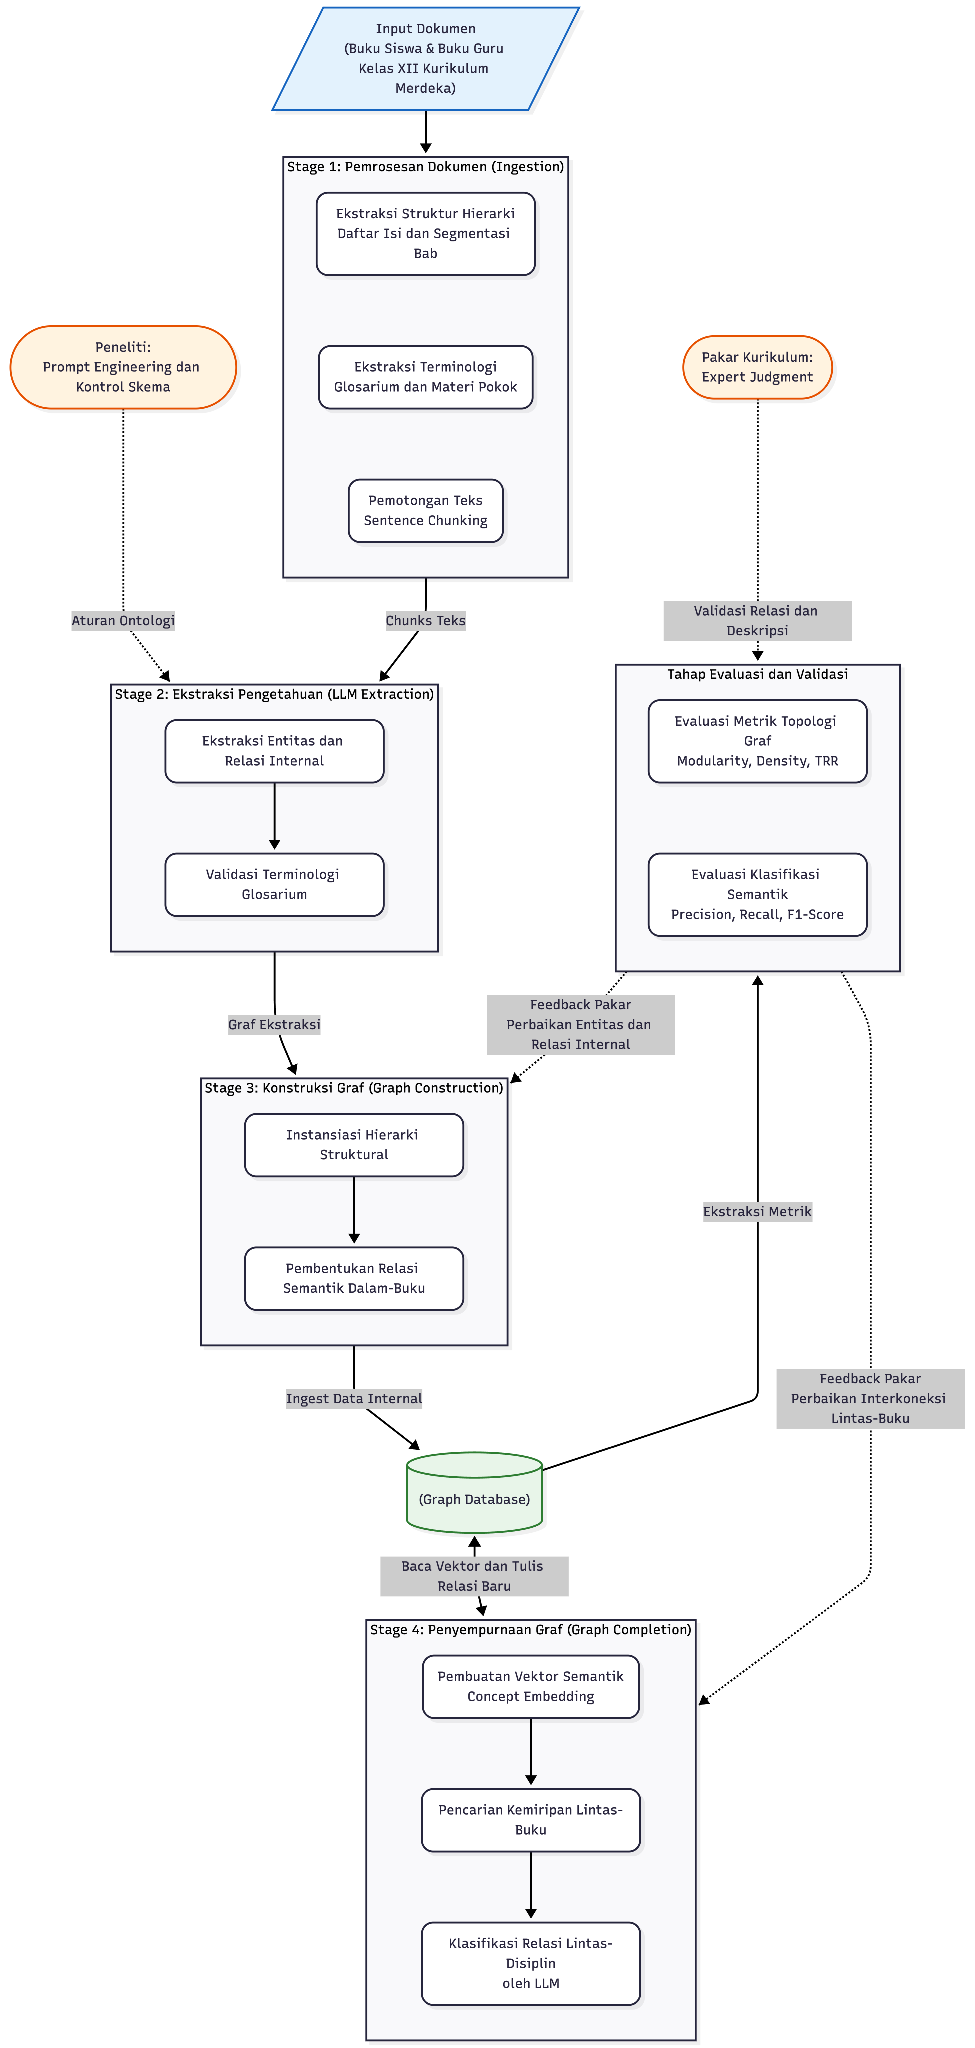
\includegraphics[width=3.33543in,height=7.02403in]{images/media/image7.png}

Gambar 3.1 Pipeline KG Construction \& Completion

\begin{enumerate}
\def\labelenumi{\arabic{enumi}.}
\item
  \textbf{Tahap 1:} Pemrosesan Dokumen (\emph{Ingestion}) -- Tahap ini
  berfokus pada pengubahan dokumen buku teks siswa dan guru (PDF) ke
  dalam format terstruktur, meliputi segmentasi hierarki bab, ekstraksi
  terminologi glosarium, dan pemotongan teks (sentence chunking).
\item
  \textbf{Tahap 2:} Ekstraksi Pengetahuan (\emph{LLM Extraction}) --
  Menggunakan model LLM terpandu (schema-constrained) untuk mengekstrak
  entitas konsep dan memetakan relasi internal (dalam-buku), yang
  divalidasi dengan terminologi glosarium.
\item
  \textbf{Tahap 3:} Konstruksi Graf (\emph{Graph Construction}) --
  Menginstansiasi hierarki struktural dan relasi semantik dalam-buku ke
  dalam basis data Knowledge Graph (Neo4j).
\item
  \textbf{Fase Evaluasi 1 (Validasi Intra-Mapel \& LLM-as-a-judge)} --
  Pada fase ini, kerangka kerja LLM-as-a-judge (Gambar 3.2) diterapkan
  untuk mengevaluasi kumpulan triple di dalam satu mata pelajaran.
  Sistem membandingkan opini dua pakar, jika terjadi ketidaksepakatan
  (\emph{disagreement}), AI Judge dipanggil sebagai penengah menggunakan
  landasan buku sebagai konteks untuk memperbaiki KG sebelum proses
  \emph{completion}. Selain itu, apabila pakar mengidentifikasi adanya
  triple yang terlewat dari KG, LLM akan mengevaluasi kesesuaian usulan
  penambahan dari kedua pakar. Jika terdapat ketidaksepakatan terhadap
  usulan tersebut, LLM akan memutuskan apakah triple baru tersebut layak
  diintegrasikan ke dalam KG atau diabaikan.
\end{enumerate}

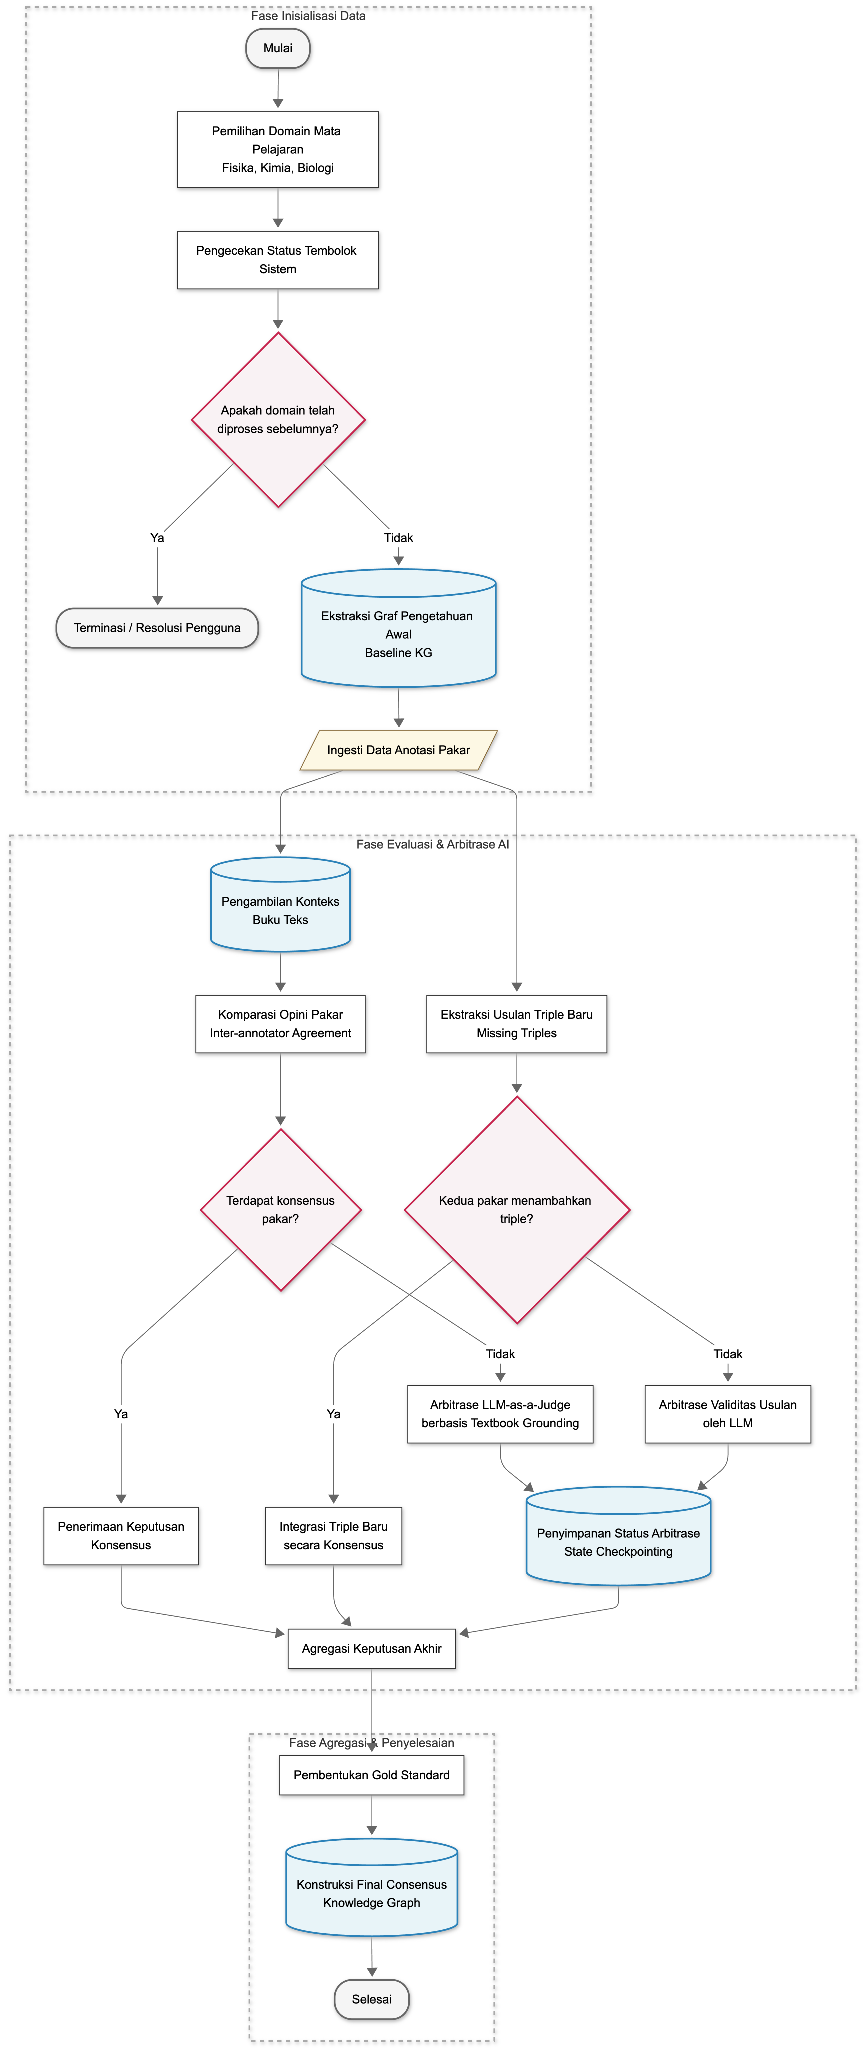
\includegraphics[width=3.59476in,height=8.50104in]{images/media/image8.png}

Gambar 3.2 Pipeline LLM-as-a-judge

\begin{enumerate}
\def\labelenumi{\arabic{enumi}.}
\setcounter{enumi}{4}
\item
  \textbf{Tahap 4:} Penyempurnaan Graf (\emph{Graph Completion}) --
  Membangun vektor semantik (\emph{concept embedding}) dari konsep yang
  ada, mencari kemiripan lintas-buku, dan menggunakan LLM sebagai
  pengklasifikasi untuk memprediksi relasi antar-disiplin ilmu.
\item
  \textbf{Fase Evaluasi 2 (Validasi Inter-Mapel \& Diskusi Pakar) --}
  Fase ini dikhususkan untuk memverifikasi \emph{edge} atau relasi
  lintas-disiplin baru yang ditambahkan oleh proses KGC. Mengingat
  relasi ini bersifat implisit, penyelesaian konflik tidak menggunakan
  AI, melainkan melalui diskusi panel yang melibatkan seluruh pakar
  untuk mencapai konsensus keilmuan yang komprehensif.

  \begin{enumerate}
  \def\labelenumii{\arabic{enumii}.}
  \item ~
    \hypertarget{skema-ontologi-knowledge-graph}{%
    \subsubsection{Skema Ontologi Knowledge
    Graph}\label{skema-ontologi-knowledge-graph}}
  \end{enumerate}
\end{enumerate}

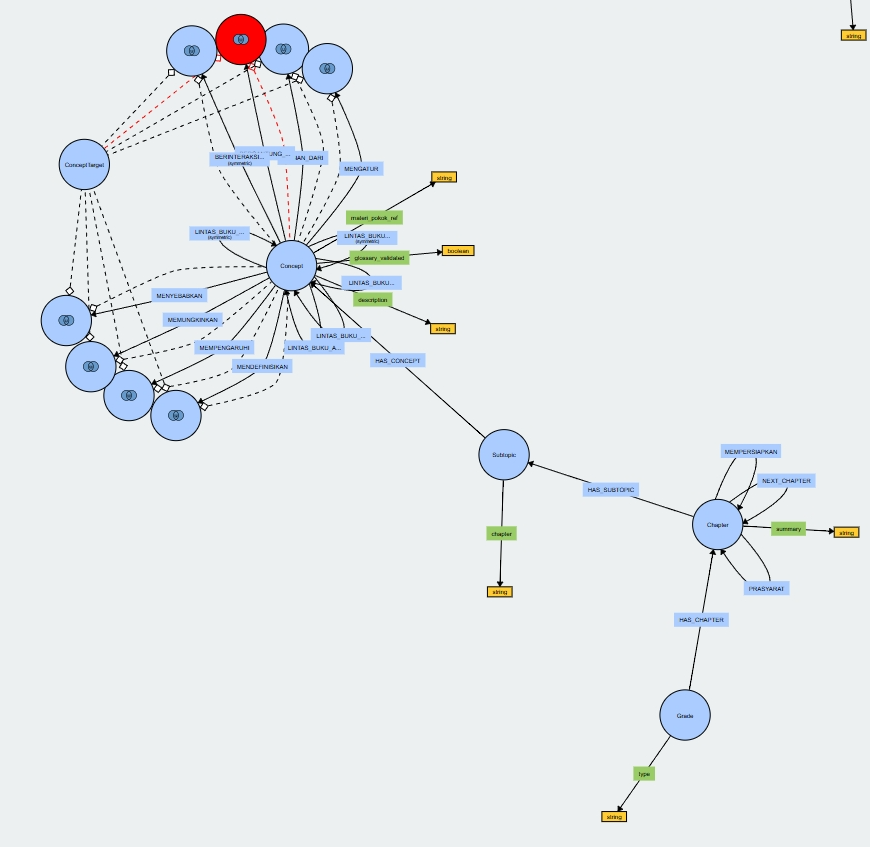
\includegraphics[width=5.5in,height=5.30206in]{images/media/image9.png}

Gambar 3.3 Skema Ontologi Knowledge Graph

Mengacu pada definisi Studer et al. (1998) yang memperluas gagasan
Gruber (1993), ontologi dipahami sebagai spesifikasi formal dan
eksplisit atas sebuah konseptualisasi bersama terhadap suatu domain.
Dalam kerangka tersebut, ontologi penelitian ini diposisikan secara
spesifik sebagai model konseptual yang bersifat deskriptif, bukan
preskriptif. Artinya, ontologi merepresentasikan konsep-konsep sains
beserta keterkaitan semantik di antaranya sebagaimana tersaji dalam buku
teks Kurikulum Merdeka, dan tidak dimaksudkan untuk merekomendasikan
urutan maupun jalur belajar tertentu.

Graf yang dihasilkan dengan demikian memodelkan struktur pengetahuan
domain, yakni keterkaitan logis antar-konsep, dan bukan strategi
pembelajaran yang mengatur bagaimana konsep tersebut sebaiknya
dipelajari. Sebagai konsekuensinya, relasi berarah seperti
PRASYARAT\_UNTUK dimaknai sebagai ketergantungan konseptual yang
terkandung dalam materi --- bahwa pemahaman satu konsep secara logis
mengandaikan konsep lain --- bukan sebagai anjuran kronologis bagi
siswa. Pembatasan epistemologis ini ditetapkan agar klaim penelitian
tetap sepadan dengan apa yang benar-benar direpresentasikan oleh sistem.

Skema knowledge graph yang digunakan dalam penelitian ini diformalkan
sebagai ontologi OWL untuk memastikan konsistensi struktur dan
vokabulari relasi antar-tahap pipeline (ekstraksi, konstruksi, dan
completion). Ontologi ini terdiri dari empat kelas struktural utama,
satu kelas pendukung untuk forward reference, serta dua keluarga relasi
semantik antar-konsep (dalam-buku dan lintas-buku).

Hierarki struktural mengikuti rantai berikut:

Grade → Chapter → Subtopic → Concept, dihubungkan oleh relasi struktural
HAS\_CHAPTER, HAS\_SUBTOPIC, dan HAS\_CONCEPT. Pada tingkat Chapter,
terdapat tiga relasi pedagogis tambahan --- NEXT\_CHAPTER (urutan baca),
PRASYARAT (ketergantungan pembelajaran), dan MEMPERSIAPKAN (kebalikan
logis dari PRASYARAT) --- yang mengkodekan struktur pedagogis buku teks.
Node Concept bersifat shared lintas-dokumen melalui operasi MERGE
berdasarkan nama, sehingga konsep yang muncul di lebih dari satu buku
teks diwakili oleh satu node --- fondasi untuk penemuan keterkaitan
lintas-disiplin pada tahap completion.

Vokabulari relasi semantik antar-konsep dibagi menjadi dua kelompok
dengan peran berbeda dalam pipeline:

\begin{enumerate}
\def\labelenumi{\arabic{enumi}.}
\item
  \begin{quote}
  Relasi dalam-buku (within-book) --- delapan tipe yang ditegakkan oleh
  prompt LLM saat ekstraksi per-Bab. Tipe relasi ini menangkap struktur
  konseptual lokal dalam satu mata pelajaran (lihat Tabel 3.1).
  \end{quote}
\item
  \begin{quote}
  Relasi lintas-buku (LINTAS\_BUKU\_*) --- lima tipe yang dihasilkan
  pada tahap completion lintas-disiplin. Relasi ini menangkap
  interkoneksi semantik antar-mata-pelajaran (Fisika, Kimia, Biologi)
  yang tidak tersurat dalam teks satu buku tunggal (lihat Tabel 3.2).
  \end{quote}
\end{enumerate}

Untuk menampung forward reference --- konsep yang disebutkan sebagai
target relasi tetapi belum diekstrak sebagai Concept lengkap ---
digunakan kelas pendukung ConceptTarget. Simpul ConceptTarget bersifat
sementara dan akan dipromosi menjadi Concept saat ekstraksi berikutnya
menemukan deskripsi lengkapnya. Skema lengkap ontologi ditunjukkan pada
Gambar 3.3.

\begin{longtable}[]{@{}
  >{\raggedright\arraybackslash}p{(\columnwidth - 4\tabcolsep) * \real{0.3333}}
  >{\raggedright\arraybackslash}p{(\columnwidth - 4\tabcolsep) * \real{0.3333}}
  >{\raggedright\arraybackslash}p{(\columnwidth - 4\tabcolsep) * \real{0.3333}}@{}}
\toprule()
\begin{minipage}[b]{\linewidth}\raggedright
\textbf{Tipe Relasi}
\end{minipage} & \begin{minipage}[b]{\linewidth}\raggedright
\textbf{Semantik}
\end{minipage} & \begin{minipage}[b]{\linewidth}\raggedright
\textbf{Sifat}
\end{minipage} \\
\begin{minipage}[b]{\linewidth}\raggedright
BAGIAN\_DARI
\end{minipage} & \begin{minipage}[b]{\linewidth}\raggedright
A merupakan bagian dari B (komposisi/hierarki)
\end{minipage} & \begin{minipage}[b]{\linewidth}\raggedright
asimetris, hierarkis
\end{minipage} \\
\begin{minipage}[b]{\linewidth}\raggedright
MENYEBABKAN
\end{minipage} & \begin{minipage}[b]{\linewidth}\raggedright
A menyebabkan B (kausasi)
\end{minipage} & \begin{minipage}[b]{\linewidth}\raggedright
asimetris
\end{minipage} \\
\begin{minipage}[b]{\linewidth}\raggedright
BERGANTUNG\_PADA
\end{minipage} & \begin{minipage}[b]{\linewidth}\raggedright
A bergantung pada B (dependensi fungsional)
\end{minipage} & \begin{minipage}[b]{\linewidth}\raggedright
asimetris
\end{minipage} \\
\begin{minipage}[b]{\linewidth}\raggedright
MENDEFINISIKAN
\end{minipage} & \begin{minipage}[b]{\linewidth}\raggedright
A mendefinisikan B (definisional)
\end{minipage} & \begin{minipage}[b]{\linewidth}\raggedright
asimetris
\end{minipage} \\
\begin{minipage}[b]{\linewidth}\raggedright
MEMPENGARUHI
\end{minipage} & \begin{minipage}[b]{\linewidth}\raggedright
A mempengaruhi B (pengaruh umum)
\end{minipage} & \begin{minipage}[b]{\linewidth}\raggedright
asimetris
\end{minipage} \\
\begin{minipage}[b]{\linewidth}\raggedright
BERINTERAKSI\_DENGAN
\end{minipage} & \begin{minipage}[b]{\linewidth}\raggedright
A dan B berinteraksi resiprokal
\end{minipage} & \begin{minipage}[b]{\linewidth}\raggedright
simetris
\end{minipage} \\
\begin{minipage}[b]{\linewidth}\raggedright
MEMUNGKINKAN
\end{minipage} & \begin{minipage}[b]{\linewidth}\raggedright
A memungkinkan B terjadi/berfungsi (\emph{enablement})
\end{minipage} & \begin{minipage}[b]{\linewidth}\raggedright
asimetris
\end{minipage} \\
\begin{minipage}[b]{\linewidth}\raggedright
MENGATUR
\end{minipage} & \begin{minipage}[b]{\linewidth}\raggedright
A mengatur atau mengontrol perilaku B (regulasi)
\end{minipage} & \begin{minipage}[b]{\linewidth}\raggedright
asimetris
\end{minipage} \\
\midrule()
\endhead
\bottomrule()
\end{longtable}

\textbf{Tabel 3.1} Vokabulari Relasi Dalam-Buku (Concept ↔ Concept)

\begin{longtable}[]{@{}
  >{\raggedright\arraybackslash}p{(\columnwidth - 4\tabcolsep) * \real{0.3333}}
  >{\raggedright\arraybackslash}p{(\columnwidth - 4\tabcolsep) * \real{0.3333}}
  >{\raggedright\arraybackslash}p{(\columnwidth - 4\tabcolsep) * \real{0.3333}}@{}}
\toprule()
\begin{minipage}[b]{\linewidth}\raggedright
\textbf{Tipe Relasi}
\end{minipage} & \begin{minipage}[b]{\linewidth}\raggedright
\textbf{Semantik}
\end{minipage} & \begin{minipage}[b]{\linewidth}\raggedright
\textbf{Sifat}
\end{minipage} \\
\begin{minipage}[b]{\linewidth}\raggedright
LINTAS\_BUKU\_SAMA\_DENGAN
\end{minipage} & \begin{minipage}[b]{\linewidth}\raggedright
Konsep di buku berbeda merujuk pada entitas yang sama
\end{minipage} & \begin{minipage}[b]{\linewidth}\raggedright
simetris
\end{minipage} \\
\begin{minipage}[b]{\linewidth}\raggedright
LINTAS\_BUKU\_APLIKASI\_DARI
\end{minipage} & \begin{minipage}[b]{\linewidth}\raggedright
Konsep A adalah penerapan konsep B di disiplin lain
\end{minipage} & \begin{minipage}[b]{\linewidth}\raggedright
asimetris
\end{minipage} \\
\begin{minipage}[b]{\linewidth}\raggedright
LINTAS\_BUKU\_PRASYARAT\_UNTUK
\end{minipage} & \begin{minipage}[b]{\linewidth}\raggedright
Konsep A prasyarat pemahaman konsep B di mata pelajaran lain
\end{minipage} & \begin{minipage}[b]{\linewidth}\raggedright
asimetris, hierarkis
\end{minipage} \\
\begin{minipage}[b]{\linewidth}\raggedright
LINTAS\_BUKU\_MEMPERDALAM
\end{minipage} & \begin{minipage}[b]{\linewidth}\raggedright
Konsep A memperdalam/memperluas pemahaman konsep B
\end{minipage} & \begin{minipage}[b]{\linewidth}\raggedright
asimetris
\end{minipage} \\
\begin{minipage}[b]{\linewidth}\raggedright
LINTAS\_BUKU\_BERKAITAN\_DENGAN
\end{minipage} & \begin{minipage}[b]{\linewidth}\raggedright
Berkaitan secara umum (\emph{fallback})
\end{minipage} & \begin{minipage}[b]{\linewidth}\raggedright
simetris
\end{minipage} \\
\midrule()
\endhead
\bottomrule()
\end{longtable}

\textbf{Tabel 3.2} Vokabulari Relasi Lintas-Buku (Cross-disciplinary)

\hypertarget{section-4}{%
\subsection{\texorpdfstring{\hfill\break
}{ }}\label{section-4}}

\textbf{3.6 Parameter Sistem dan Definisi Operasional}

\textbf{3.6.1 Parameter Sistem}

Parameter dalam penelitian ini adalah parameter pipeline yang dapat
dimodifikasi oleh peneliti dan memengaruhi karakteristik knowledge graph
yang ddihasilkan. Variabel-variabel tersebut meliputi: Parameter Sistem
dan Definisi Operasional (Bab 3

\begin{longtable}[]{@{}
  >{\raggedright\arraybackslash}p{(\columnwidth - 4\tabcolsep) * \real{0.3333}}
  >{\raggedright\arraybackslash}p{(\columnwidth - 4\tabcolsep) * \real{0.3333}}
  >{\raggedright\arraybackslash}p{(\columnwidth - 4\tabcolsep) * \real{0.3333}}@{}}
\toprule()
\begin{minipage}[b]{\linewidth}\raggedright
\textbf{Parameter}
\end{minipage} & \begin{minipage}[b]{\linewidth}\raggedright
\textbf{Deskripsi}
\end{minipage} & \begin{minipage}[b]{\linewidth}\raggedright
\textbf{Nilai/Level}
\end{minipage} \\
\begin{minipage}[b]{\linewidth}\raggedright
Model LLM Ekstraksi
\end{minipage} & \begin{minipage}[b]{\linewidth}\raggedright
Model bahasa besar yang digunakan untuk ekstraksi konsep
\end{minipage} & \begin{minipage}[b]{\linewidth}\raggedright
gemini-2.5-flash
\end{minipage} \\
\begin{minipage}[b]{\linewidth}\raggedright
Strategi \emph{Prompt Engineering}
\end{minipage} & \begin{minipage}[b]{\linewidth}\raggedright
Variasi instruksi sistem untuk ekstraksi
\end{minipage} & \begin{minipage}[b]{\linewidth}\raggedright
Structured schema prompt + context injection + strict output constraints
\end{minipage} \\
\begin{minipage}[b]{\linewidth}\raggedright
Model \emph{Embedding}
\end{minipage} & \begin{minipage}[b]{\linewidth}\raggedright
Model representasi vektor untuk perhitungan similaritas
\end{minipage} & \begin{minipage}[b]{\linewidth}\raggedright
Gemini Embedding, text-embedding-3-small, multilingual-e5-small
\end{minipage} \\
\begin{minipage}[b]{\linewidth}\raggedright
Threshold Similaritas
\end{minipage} & \begin{minipage}[b]{\linewidth}\raggedright
Nilai ambang batas cosine similarity untuk KGC
\end{minipage} & \begin{minipage}[b]{\linewidth}\raggedright
0.7 - 0.9 (default: 0.8)
\end{minipage} \\
\begin{minipage}[b]{\linewidth}\raggedright
Parameter Chunking Dokumen
\end{minipage} & \begin{minipage}[b]{\linewidth}\raggedright
Pemotongan dokumen sebelum ekstraksi agar konteks stabil
\end{minipage} & \begin{minipage}[b]{\linewidth}\raggedright
chunk\_size = 800, chunk\_overlap = 200
\end{minipage} \\
\begin{minipage}[b]{\linewidth}\raggedright
Sumber Data Buku
\end{minipage} & \begin{minipage}[b]{\linewidth}\raggedright
Variasi domain materi yang diproses pipeline
\end{minipage} & \begin{minipage}[b]{\linewidth}\raggedright
Biologi Kelas XII, Fisika Kelas XII, Kimia Kelas XII
\end{minipage} \\
\midrule()
\endhead
\bottomrule()
\end{longtable}

\hypertarget{section-5}{%
\paragraph{}\label{section-5}}

\hypertarget{metrik-evaluasi}{%
\paragraph{3.6.3 Metrik Evaluasi}\label{metrik-evaluasi}}

Metrik Evaluasi dalam penelitian ini meliputi:

\begin{longtable}[]{@{}
  >{\raggedright\arraybackslash}p{(\columnwidth - 4\tabcolsep) * \real{0.3333}}
  >{\raggedright\arraybackslash}p{(\columnwidth - 4\tabcolsep) * \real{0.3333}}
  >{\raggedright\arraybackslash}p{(\columnwidth - 4\tabcolsep) * \real{0.3333}}@{}}
\toprule()
\begin{minipage}[b]{\linewidth}\raggedright
\textbf{Variabel}
\end{minipage} & \begin{minipage}[b]{\linewidth}\raggedright
\textbf{Deskripsi}
\end{minipage} & \begin{minipage}[b]{\linewidth}\raggedright
\textbf{Satuan}
\end{minipage} \\
\begin{minipage}[b]{\linewidth}\raggedright
Jumlah Konsep Terekstrak
\end{minipage} & \begin{minipage}[b]{\linewidth}\raggedright
Total konsep yang berhasil diekstrak per dokumen
\end{minipage} & \begin{minipage}[b]{\linewidth}\raggedright
Jumlah node
\end{minipage} \\
\begin{minipage}[b]{\linewidth}\raggedright
Jumlah Relasi Terprediksi
\end{minipage} & \begin{minipage}[b]{\linewidth}\raggedright
Total relasi implisit yang ditemukan melalui KGC
\end{minipage} & \begin{minipage}[b]{\linewidth}\raggedright
Jumlah edge
\end{minipage} \\
\begin{minipage}[b]{\linewidth}\raggedright
\emph{Average Degree Centrality} (ADC)
\end{minipage} & \begin{minipage}[b]{\linewidth}\raggedright
Rata-rata degree centrality node dalam graf
\end{minipage} & \begin{minipage}[b]{\linewidth}\raggedright
Nilai 0-1
\end{minipage} \\
\begin{minipage}[b]{\linewidth}\raggedright
\emph{Modularity}
\end{minipage} & \begin{minipage}[b]{\linewidth}\raggedright
Ukuran struktur komunitas dalam graf
\end{minipage} & \begin{minipage}[b]{\linewidth}\raggedright
Nilai -0.5 hingga 1
\end{minipage} \\
\begin{minipage}[b]{\linewidth}\raggedright
Tingkat Validitas Pakar
\end{minipage} & \begin{minipage}[b]{\linewidth}\raggedright
Persentase relasi yang divalidasi benar oleh pakar
\end{minipage} & \begin{minipage}[b]{\linewidth}\raggedright
Persentase (\%)
\end{minipage} \\
\midrule()
\endhead
\bottomrule()
\end{longtable}

\hypertarget{definisi-operasional}{%
\subsubsection{3.6.4 Definisi Operasional}\label{definisi-operasional}}

\textbf{Tabel 3.3 Definisi Operasional Istilah Penelitian}

\begin{longtable}[]{@{}
  >{\raggedright\arraybackslash}p{(\columnwidth - 2\tabcolsep) * \real{0.2652}}
  >{\raggedright\arraybackslash}p{(\columnwidth - 2\tabcolsep) * \real{0.7348}}@{}}
\toprule()
\begin{minipage}[b]{\linewidth}\raggedright
\textbf{Istilah}
\end{minipage} & \begin{minipage}[b]{\linewidth}\raggedright
\textbf{Definisi Operasional}
\end{minipage} \\
\begin{minipage}[b]{\linewidth}\raggedright
\emph{Knowledge Graph}
\end{minipage} & \begin{minipage}[b]{\linewidth}\raggedright
Struktur data graf dalam Neo4j yang terdiri dari node dengan label
MataPelajaran, Document, Bab, SubBab, SubSubBab, Konsep, SubKonsep dan
edge berupa relasi struktural (hasBab, hasKonsep, dll.) maupun semantik
(SIMILAR\_TO, isPrerequisiteOf, supports, analogousTo)
\end{minipage} \\
\begin{minipage}[b]{\linewidth}\raggedright
Konsep
\end{minipage} & \begin{minipage}[b]{\linewidth}\raggedright
Entitas pengetahuan fisika/kimia/biologi yang memiliki nama, dan
deskripsi
\end{minipage} \\
\begin{minipage}[b]{\linewidth}\raggedright
SubKonsep
\end{minipage} & \begin{minipage}[b]{\linewidth}\raggedright
Konten terperinci yang menjelaskan atau mengelaborasi sebuah Konsep,
memiliki atribut nama, dan deskripsi.
\end{minipage} \\
\begin{minipage}[b]{\linewidth}\raggedright
Relasi Struktural
\end{minipage} & \begin{minipage}[b]{\linewidth}\raggedright
Hubungan hierarkis dalam graf: MataPelajaran → Document → Bab → SubBab →
SubSubBab → Konsep → SubKonsep
\end{minipage} \\
\begin{minipage}[b]{\linewidth}\raggedright
Relasi Implisit
\end{minipage} & \begin{minipage}[b]{\linewidth}\raggedright
Hubungan antar-konsep yang tidak tertulis eksplisit dalam teks buku
tetapi dapat diinferensikan melalui analisis semantik LLM
\end{minipage} \\
\begin{minipage}[b]{\linewidth}\raggedright
KGC (\emph{Knowledge Graph Completion})
\end{minipage} & \begin{minipage}[b]{\linewidth}\raggedright
Proses prediksi triple (head, relation, tail) yang hilang menggunakan
embedding similarity dan klasifikasi LLM untuk menghasilkan relasi
isPrerequisiteOf, supports, atau analogousTo
\end{minipage} \\
\begin{minipage}[b]{\linewidth}\raggedright
\emph{Embedding}
\end{minipage} & \begin{minipage}[b]{\linewidth}\raggedright
Representasi vektor numerik dari deskripsi konsep yang dihasilkan oleh
model embedding (dimensi bervariasi tergantung model)
\end{minipage} \\
\begin{minipage}[b]{\linewidth}\raggedright
\emph{Cosine Similarity}
\end{minipage} & \begin{minipage}[b]{\linewidth}\raggedright
Ukuran kemiripan antara dua vektor embedding, dihitung sebagai dot
product dibagi produktus norma kedua vektor
\end{minipage} \\
\begin{minipage}[b]{\linewidth}\raggedright
Vector Index / ANN
\end{minipage} & \begin{minipage}[b]{\linewidth}\raggedright
ANN

Struktur indeks pada basis data Neo4j yang menggunakan algoritma
Approximate Nearest Neighbor (ANN) untuk mempercepat pencarian node
Konsep yang memiliki cosine similarity tinggi tanpa harus membandingkan
seluruh pasangan node secara brute-force O(n2).
\end{minipage} \\
\begin{minipage}[b]{\linewidth}\raggedright
In-Context Learning (ICL)
\end{minipage} & \begin{minipage}[b]{\linewidth}\raggedright
Strategi pemanfaatan Large Language Model (LLM) dengan memberikan
demonstrasi struktur ontologi (Knowledge Prompt) di dalam instruksi
tanpa memerlukan proses fine-tuning model untuk memprediksi relasi.
\end{minipage} \\
\begin{minipage}[b]{\linewidth}\raggedright
Average Degree Centrality (ADC)
\end{minipage} & \begin{minipage}[b]{\linewidth}\raggedright
Metrik evaluasi struktural yang mengukur rata-rata jumlah koneksi
(derajat) per node untuk memvalidasi tingkat kepadatan interkoneksi
materi sains dalam graf.
\end{minipage} \\
\begin{minipage}[b]{\linewidth}\raggedright
\end{minipage} & \begin{minipage}[b]{\linewidth}\raggedright
\end{minipage} \\
\begin{minipage}[b]{\linewidth}\raggedright
\end{minipage} & \begin{minipage}[b]{\linewidth}\raggedright
\end{minipage} \\
\midrule()
\endhead
\bottomrule()
\end{longtable}

\hypertarget{teknik-pengumpulan-data}{%
\subsection{3.7 Teknik Pengumpulan Data}\label{teknik-pengumpulan-data}}

\hypertarget{jenis-data}{%
\subsubsection{3.7.1 Jenis Data}\label{jenis-data}}

Penelitian ini menggunakan dua jenis data yang saling melengkapi, yaitu
data primer berupa dokumen kurikulum sebagai sumber ekstraksi
pengetahuan, dan data validasi berupa penilaian pakar terhadap triple
relasi yang dihasilkan sistem. Data primer dimanfaatkan pada tahap
konstruksi dan pelengkapan knowledge graph (Tahap 1--4), sedangkan data
validasi digunakan pada tahap evaluasi (Tahap 5) untuk mengukur akurasi
dan kelengkapan relasi yang diprediksi sistem dari sudut pandang
pedagogis.

\hypertarget{data-primer-kurikulum}{%
\paragraph{3.7.2 Data Primer Kurikulum}\label{data-primer-kurikulum}}

Data primer penelitian ini berupa berkas PDF buku teks elektronik resmi
dari Kementerian Pendidikan, Kebudayaan, Riset, dan Teknologi
(Kemendikbudristek) yang diperoleh melalui repositori
https://buku.kemdikbud.go.id. Tiga buku teks untuk mata pelajaran
Fisika, Kimia, dan Biologi jenjang Kelas XII Fase F digunakan sebagai
sumber ekstraksi pengetahuan untuk membangun knowledge graph kurikulum
sains.

\hypertarget{data-validasi-pakar}{%
\paragraph{3.7.3 Data Validasi Pakar}\label{data-validasi-pakar}}

Data validasi diperoleh melalui penilaian pakar (expert review) terhadap
triple relasi yang dihasilkan sistem. Setiap triple dinilai menggunakan
skala empat poin: Benar (relasi tepat dan relevan), Sebagian benar
(relasi relevan namun perlu perbaikan), Salah (relasi tidak tepat), dan
Kurang konteks (relasi yang seharusnya ada namun tidak ditemukan
sistem). Reviewer juga dapat menambahkan triple yang dianggap hilang
(missing triples) serta komentar per relasi.

\hypertarget{section-6}{%
\subsubsection{\texorpdfstring{\hfill\break
}{ }}\label{section-6}}

\hypertarget{cara-pengumpulan-data}{%
\subsubsection{3.7.4 Cara Pengumpulan
Data}\label{cara-pengumpulan-data}}

Pengumpulan data validasi dilakukan melalui aplikasi web KG Review App
yang dikembangkan khusus untuk penelitian ini. Aplikasi ini dibangun
menggunakan Next.js karena jumlah item penilaian melebihi 100 triple per
mata pelajaran, sehingga tidak memungkinkan penggunaan Google Forms yang
memiliki keterbatasan kapasitas tampilan dan navigasi untuk kuesioner
skala besar. Penjelasan teknis dan visualisasi antarmuka dari aplikasi
ini akan dibahas secara mendalam pada Bab 4.

Alur pengumpulan data adalah sebagai berikut:

\begin{enumerate}
\def\labelenumi{\arabic{enumi}.}
\item
  Peneliti mengunggah hasil knowledge graph dalam format JSON ke panel
  admin aplikasi
\item
  Peneliti mempublikasikan mata pelajaran sehingga dapat diakses oleh
  reviewer
\item
  Reviewer menerima kredensial login yang diberikan peneliti
\item
  Reviewer masuk ke aplikasi, memilih mata pelajaran yang ditugaskan,
  dan menilai setiap triple relasi menggunakan skala empat poin
\item
  Reviewer dapat menambahkan triple yang dirasa hilang (missing triples)
  dan memberikan komentar per relasi
\item
  Setelah seluruh triple dinilai, reviewer mengonfirmasi penyelesaian
  review
\end{enumerate}

Terdapat dua reviewer per mata pelajaran (total 6 reviewer untuk Fisika,
Kimia, dan Biologi), sehingga setiap triple mendapatkan penilaian dari
dua pakar independen.

\hypertarget{pengolahan-data}{%
\subsection{3.8 Pengolahan Data}\label{pengolahan-data}}

Data rating dari setiap reviewer diolah untuk menghasilkan tiga metrik
evaluasi per bab per mata pelajaran, yaitu \emph{Precision},
\emph{Recall}, dan \emph{F1-Score} yang dihitung menggunakan formulasi
matematis yang telah dijelaskan pada Subbab 2.2.4. Selain itu, dihitung
\emph{inter-rater agreement} antar penilai menggunakan Gwet's AC1 untuk
mengukur konsistensi penilaian.

\hypertarget{analisis-data}{%
\subsection{3.9 Analisis Data}\label{analisis-data}}

Analisis data dalam penelitian ini dilakukan melalui tiga pendekatan
yang saling melengkapi, yaitu analisis struktural berbasis metrik graf,
analisis validasi pakar, dan analisis komparatif lintas mata pelajaran.
Ketiga pendekatan ini dirancang untuk menjawab rumusan masalah
penelitian secara komprehensif, baik dari sisi kuantitatif objektif
maupun validitas pedagogis yang bersifat kualitatif.

\hypertarget{analisis-struktural-graph-metrics}{%
\subsubsection{3.9.1 Analisis Struktural (Graph
Metrics)}\label{analisis-struktural-graph-metrics}}

Analisis struktural bertujuan untuk mengukur perubahan karakteristik
topologi Knowledge Graph secara kuantitatif, khususnya untuk
mengevaluasi dampak proses Knowledge Graph Completion (KGC) terhadap
kualitas interkoneksi antar-konsep yang dihasilkan. Analisis ini
dilakukan dengan membandingkan nilai metrik graf pada dua kondisi, yaitu
sebelum KGC (graf awal hasil ekstraksi LLM) dan sesudah KGC (graf yang
telah diperkaya dengan relasi implisit lintas disiplin).

Metrik yang dihitung pada kedua kondisi tersebut meliputi Average Degree
Centrality (ADC), Graph Density, Modularity, Typed Relation Ratio, dan
Description Completeness, sebagaimana telah didefinisikan secara
operasional pada Subbab 3.6. Seluruh nilai metrik diperoleh melalui
eksekusi kueri Cypher pada basis data Neo4j Aura, sehingga
perhitungannya bersifat deterministik dan dapat direproduksi.

Hasil perbandingan pre-KGC dan post-KGC disajikan dalam bentuk tabel
berpasangan per mata pelajaran (Fisika, Kimia, dan Biologi). Peningkatan
nilai ADC dan Graph Density setelah proses KGC diinterpretasikan sebagai
indikator bahwa relasi implisit yang diprediksi oleh LLM berhasil
memperkaya kepadatan jaringan pengetahuan. Sebaliknya, penurunan nilai
Modularity yang terlalu drastis dapat mengindikasikan bahwa batas
komunitas antar-bab menjadi kabur akibat relasi lintas disiplin yang
terlalu agresif, sehingga perlu dikaji lebih lanjut melalui validasi
pakar.

Selain perbandingan pre-post, analisis ini juga mencakup pemeriksaan
distribusi tipe relasi yang dihasilkan (isPrerequisiteOf, supports,
analogousTo) untuk mengetahui pola relasi implisit yang paling dominan
ditemukan sistem pada setiap mata pelajaran.

\hypertarget{analisis-validasi-pakar-expert-validation-analysis}{%
\subsubsection{3.9.2 Analisis Validasi Pakar (Expert Validation
Analysis)}\label{analisis-validasi-pakar-expert-validation-analysis}}

Analisis ini bertujuan untuk mengukur akurasi dan kelengkapan konsep
yang telah dihasilkan KG. Sebelum dilakukan perhitungan performa,
tingkat kesepakatan awal antar-pakar (\emph{inter-rater reliability})
diukur menggunakan metrik Gwet's AC1 untuk mengakomodasi distribusi
label evaluasi yang cenderung tidak seimbang (\emph{imbalanced}) pada
prediksi LLM. Setelah itu, \emph{ground truth} final dibentuk
berdasarkan konsensus evaluasi \emph{hybrid}. Kinerja ekstraksi sistem
kemudian dievaluasi terhadap \emph{ground truth} tersebut menggunakan
modifikasi Fuzzy Precision and Recall dan berdasarkan pemetaan nilai
keanggotaan yang disebutkan pada subbab 2.2.4.

\hypertarget{analisis-komparatif-comparative-analysis}{%
\subsubsection{3.9.3 Analisis Komparatif (Comparative
Analysis)}\label{analisis-komparatif-comparative-analysis}}

Analisis komparatif bertujuan untuk membandingkan kualitas Knowledge
Graph yang dihasilkan di antara ketiga mata pelajaran, yaitu Fisika,
Kimia, dan Biologi, guna mengidentifikasi perbedaan karakteristik
struktur pengetahuan antar-disiplin ilmu sains dalam konteks Kurikulum
Merdeka.

Perbandingan dilakukan pada dua dimensi secara bersamaan. Pertama,
dimensi struktural membandingkan nilai metrik graf (ADC, Density,
Modularity, Typed Relation Ratio) antar ketiga mata pelajaran pada
kondisi post-KGC. Perbedaan nilai metrik antar mata pelajaran
diinterpretasikan sebagai cerminan perbedaan kepadatan koneksi
konseptual dan struktur komunitas topik yang inheren pada masing-masing
disiplin ilmu. Sebagai contoh, Biologi yang memiliki banyak hierarki
taksonomi dan proses fisiologis yang saling bergantung diperkirakan
menghasilkan ADC yang lebih tinggi dibandingkan Fisika yang cenderung
memiliki topik yang lebih modular.

Kedua, dimensi validasi membandingkan nilai Precision, Recall, dan F1
antar ketiga mata pelajaran. Perbedaan nilai ini dianalisis untuk
mengidentifikasi disiplin ilmu mana yang paling menguntungkan dari
pendekatan LLM-Assisted KGC, serta disiplin ilmu mana yang masih
memerlukan penyempurnaan lebih lanjut, misalnya melalui strategi prompt
engineering yang lebih spesifik per domain.

Selanjutnya, dilakukan triangulasi antara hasil metrik struktural dan
hasil validasi pakar untuk menguji koherensi antara keduanya. Jika mata
pelajaran dengan ADC tinggi juga memperoleh Precision tinggi dari
reviewer, maka hal ini memperkuat argumen bahwa kepadatan koneksi yang
dihasilkan sistem memang mencerminkan interkoneksi yang valid secara
pedagogis, bukan sekadar artefak komputasional. Hasil analisis
komparatif disajikan dalam bentuk tabel ringkasan tiga kolom (Fisika,
Kimia, Biologi) yang memuat seluruh metrik struktural dan metrik
validasi secara berdampingan untuk memudahkan perbandingan.

\hypertarget{hasil-penelitian-dan-pembahasan}{%
\section{\texorpdfstring{\hfill\break
HASIL PENELITIAN DAN
PEMBAHASAN}{ HASIL PENELITIAN DAN PEMBAHASAN}}\label{hasil-penelitian-dan-pembahasan}}

Bab ini memaparkan hasil penerapan kerangka kerja Knowledge Graph
Completion berbasis Large Language Model yang telah dirancang pada bab
sebelumnya, mulai dari pembangunan knowledge graph melalui pipeline
ekstraksi, konstruksi, dan completion, hingga evaluasi kualitasnya.
Mengikuti kerangka Design Science Research (DSR), pembahasan disusun
dengan menyajikan hasil tiap tahapan pipeline beserta artefak yang
dihasilkannya (Subbab 4.1), yang kemudian dilanjutkan dengan evaluasi
struktural graf, validasi pakar, dan pembahasan kualitatif atas kualitas
relasi lintas-buku yang ditemukan (Subbab 4.2).

\hypertarget{tahap-ingestion-pdf-parsing}{%
\subsection{4.1 Tahap Ingestion (PDF
Parsing)}\label{tahap-ingestion-pdf-parsing}}

Tahap ini mengubah \emph{e-book} PDF menjadi struktur data yang siap
diproses LLM. Output utama adalah teks per bab, metadata halaman, daftar
subbab, glosarium, dan materi pokok.

\begin{enumerate}
\def\labelenumi{\arabic{enumi}.}
\item
  \textbf{Ekstraksi teks PDF.}
\end{enumerate}

\begin{itemize}
\item
  PDF dimuat memakai SimpleDirectoryReader (LlamaIndex) dengan backend
  PyMuPDF.
\item
  Tiap halaman menjadi objek Document yang menyimpan page\_label.
\end{itemize}

\begin{enumerate}
\def\labelenumi{\arabic{enumi}.}
\setcounter{enumi}{1}
\item
  \textbf{Deteksi halaman TOC (daftar isi).}
\end{enumerate}

\begin{itemize}
\item
  Dipakai metode dua `sinyal' agar tidak salah membaca halaman konten
  sebagai TOC.
\item
  Sinyal A: ada \emph{anchor} kata seperti "daftar isi" atau "bab".
\item
  Sinyal B: ada pola \emph{leader dots} dan nomor halaman, misalnya
  ..... 191.
\item
  Halaman dianggap TOC hanya jika keduanya muncul bersamaan. Hal ini
  mencegah \emph{false positive} pada halaman konten yang sekadar
  menyebut kata "bab" atau halaman gambar yang kebetulan memuat kata
  "daftar isi" tanpa daftar nomor halaman.
\end{itemize}

\begin{enumerate}
\def\labelenumi{\arabic{enumi}.}
\setcounter{enumi}{2}
\item
  \textbf{Parsing struktur Bab dan Subbab.}
\end{enumerate}

\begin{itemize}
\item
  Pola Bab diekstrak dengan regex yang menangkap format judul -
  \emph{leader dots} - nomor halaman.

  \begin{itemize}
  \item
    Contoh: "Bab 4 Inovasi Bioteknologi..... 191"
  \end{itemize}
\item
  SubBab dicari sebagai entri bertanda huruf besar (A., B., dst.) di
  rentang TOC antara dua Bab berurutan.
\item
  Hasil parsing disusun menjadi daftar {[}\{name, page\_start,
  subchapters{[}{]}\}{]}.
\end{itemize}

\begin{enumerate}
\def\labelenumi{\arabic{enumi}.}
\setcounter{enumi}{3}
\item
  \textbf{Klasifikasi halaman TOC vs konten.}
\end{enumerate}

\begin{itemize}
\item
  Setelah deteksi awal, halaman yang terindikasi TOC digunakan untuk
  menyusun teks TOC gabungan.
\item
  Halaman konten tidak dimasukkan agar parsing bab dan subbab stabil.
\end{itemize}

\begin{enumerate}
\def\labelenumi{\arabic{enumi}.}
\setcounter{enumi}{4}
\item
  \textbf{Ekstraksi glosarium.}
\end{enumerate}

\begin{itemize}
\item
  Pencarian glosarium dilakukan pada 30 halaman terakhir dengan
  \emph{state} in\_glossary.
\item
  \emph{State} diaktifkan oleh token "glosarium" dan dimatikan oleh
  terminator seperti "indeks" atau "daftar pustaka".
\item
  Pasangan istilah dan definisi di-\emph{parse} menjadi \emph{lookup
  table}.
\item
  \emph{Lookup} ini dipakai sebagai validasi terminologi pada Tahap 2.
\end{itemize}

\begin{enumerate}
\def\labelenumi{\arabic{enumi}.}
\setcounter{enumi}{5}
\item
  \textbf{Penugasan bab ke \emph{chunk}}
\end{enumerate}

\begin{itemize}
\item
  Setiap \emph{chunk} dihubungkan ke bab berdasarkan interval halaman:
  page\_start \textless= page \textless{} next\_page.
\item
  page\_label dikonversi ke integer (termasuk angka Romawi).
\item
  Kompleksitas \(O(N \cdot C)\) untuk \(N\) chunk dan \(C\) bab, dapat
  diturunkan ke \(O(N\ log\ C)\) dengan \emph{binary search} jika skala
  membesar.
\end{itemize}

\begin{enumerate}
\def\labelenumi{\arabic{enumi}.}
\setcounter{enumi}{6}
\item
  \textbf{Ekstraksi materi pokok (Buku Guru).}
\end{enumerate}

\begin{itemize}
\item
  Untuk tiap bab, sistem mencari \emph{region} teks yang sesuai judul
  bab di Buku Guru.
\item
  Dalam region tersebut, sistem mencari penanda "Materi Pokok" dan
  mengekstrak item di sekitarnya.
\item
  Hasil materi pokok digunakan sebagai \emph{constraint} kurikulum pada
  Tahap 2 agar konsep yang diekstrak tetap sesuai kompetensi.
\end{itemize}

\hypertarget{tahap-ekstraksi-llm-prompting-schema}{%
\subsection{4.2 Tahap Ekstraksi (LLM Prompting \&
Schema)}\label{tahap-ekstraksi-llm-prompting-schema}}

Tahap ini mengubah teks yang dihasilkan Tahap 1 menjadi \emph{knowledge
graph} terstruktur melalui \emph{schema-constrained} \emph{prompting}.
Fokusnya adalah konsistensi struktur, validasi terminologi, dan
pembatasan konsep pada materi pokok.

\begin{enumerate}
\def\labelenumi{\arabic{enumi}.}
\item
  \begin{quote}
  \textbf{Text chunking.}
  \end{quote}
\end{enumerate}

\begin{quote}
SentenceSplitter (LlamaIndex) memecah dokumen dengan chunk\_size = 800
dan chunk\_overlap = 200.

\emph{Overlap} berfungsi sebagai \emph{sliding window} untuk
mempertahankan konteks lintas-\emph{chunk} di batas kalimat.
\end{quote}

\begin{enumerate}
\def\labelenumi{\arabic{enumi}.}
\setcounter{enumi}{1}
\item
  \begin{quote}
  \textbf{Per-chapter aggregation.}
  \end{quote}
\end{enumerate}

\begin{quote}
\emph{Chunk} yang ter-\emph{assign} ke bab yang sama digabung menjadi
chapter\_text.

LLM diberi konteks bab secara utuh, bukan potongan parsial per
\emph{chunk}.
\end{quote}

\begin{enumerate}
\def\labelenumi{\arabic{enumi}.}
\setcounter{enumi}{2}
\item
  \begin{quote}
  \textbf{Triplet extraction.}
  \end{quote}
\end{enumerate}

\begin{quote}
Model: Gemini 2.5 Flash Lite via Google GenAI SDK.

Prompt bersifat zero-shot dan schema-constrained.

Prompt menyertakan:

nama bab dan prev/next chapter,

daftar subchapter dari TOC,

glosarium sebagai validation set,

materi pokok sebagai \emph{curriculum constraint},

konsep dari buku lain sebagai \emph{cross-book context}.
\end{quote}

\begin{enumerate}
\def\labelenumi{\arabic{enumi}.}
\setcounter{enumi}{3}
\item
  \begin{quote}
  \textbf{Struktur prompt.}
  \end{quote}
\end{enumerate}

\begin{quote}
Prompt didefinisikan \emph{inline} di dalam notebook (cell
\emph{prompt\_template}) dan dibagi menjadi delapan blok:

Instruksi bahasa: output wajib Bahasa Indonesia, kecuali istilah ilmiah
tanpa padanan resmi.

Deklarasi hierarki graf: Kelas -\textgreater{} Bab -\textgreater{}
Subchapter -\textgreater{} Konsep.

Filter konten: abaikan daftar isi, soal latihan, glosarium, rangkuman,
dan elemen administratif.

Aturan ekstraksi konsep (8 aturan), termasuk batas 3-5 konsep per
subchapter, deskripsi 1-2 kalimat ilmiah, dan validasi materi pokok Buku
Guru.
\end{quote}

\begin{enumerate}
\def\labelenumi{\arabic{enumi}.}
\setcounter{enumi}{4}
\item
  \begin{quote}
  Daftar 15 tipe relasi dalam Bab:
  \end{quote}
\end{enumerate}

\begin{quote}
MENDEFINISIKAN, MENYEBABKAN, MEMUNGKINKAN, MENGATUR, BAGIAN\_DARI,
TERDIRI\_DARI, BERGANTUNG\_PADA, BERINTERAKSI\_DENGAN, BEREAKSI\_DENGAN,
MENGHASILKAN, MEMPENGARUHI, TERLETAK\_DI, DIFORMULASIKAN\_SEBAGAI,
DIKATALISIS\_OLEH, MEMILIKI\_SIFAT.

Instruksi \emph{cross-chapter reasoning} yang menghasilkan relasi
PRASYARAT atau MEMPERSIAPKAN dengan concept\_links antar-bab.

Skema strict JSON output: chapter\_summary,
subtopics{[}*{]}.concepts{[}*{]}, dan chapter\_relations{[}{]}.

Catatan validasi: concepts minimal 1 per subtopic,
relations{[}{]}.description wajib diisi.

Prompt bersifat \emph{zero-shot} (tanpa contoh) dan mengandalkan
struktur instruksi + penegakan skema untuk konsistensi output.
\end{quote}

\begin{enumerate}
\def\labelenumi{\arabic{enumi}.}
\setcounter{enumi}{5}
\item
  \begin{quote}
  \textbf{Structured output parsing.}
  \end{quote}
\end{enumerate}

\begin{quote}
Respons di-\emph{strip} dari \emph{fence markdown} (json/) lalu
di-\emph{decode} via json.loads.

Skema target:

chapter\_summary

subtopics{[}*{]}.concepts{[}*{]} dengan field:

name, description, glossary\_validated, materi\_pokok\_ref,
cross\_book\_links{[}{]}, relations{[}{]}
\end{quote}

\begin{enumerate}
\def\labelenumi{\arabic{enumi}.}
\setcounter{enumi}{6}
\item
  \begin{quote}
  \textbf{Post-processing validation.}
  \end{quote}
\item
  \begin{quote}
  \textbf{\hspace{0pt}\hspace{0pt}Cross-book link filtering.}
  \end{quote}
\end{enumerate}

\begin{quote}
Link ditolak jika target\_book == current\_book atau target\_book tidak
ada di daftar buku yang dimuat.

Tujuannya mencegah self-loop dan referensi dangling.
\end{quote}

\begin{enumerate}
\def\labelenumi{\arabic{enumi}.}
\setcounter{enumi}{8}
\item
  \begin{quote}
  \textbf{Heuristic fallback (}infer\_cross\_links\textbf{).}
  \end{quote}
\end{enumerate}

\begin{quote}
Jika LLM mengembalikan array kosong, jalankan matching token-overlap
gaya Jaccard.

Token yang dipakai: panjang \textgreater= 4 dan non-stopword.

Pasangan dibentuk dari (concept\_name, description) vs kandidat buku
lain.

Kriteria: \textbar overlap\textbar{} \textgreater= 2, di-rank menurun,
ambil top-K (K = 2).
\end{quote}

\begin{enumerate}
\def\labelenumi{\arabic{enumi}.}
\setcounter{enumi}{9}
\item
  \begin{quote}
  \textbf{Relation sanitization}
  \end{quote}
\end{enumerate}

\begin{quote}
triple dengan type atau target kosong dibuang.
\end{quote}

\hypertarget{graph-construction-eksekusi-neo4j-cypher}{%
\subsection{\texorpdfstring{4.3 \emph{Graph Construction} (Eksekusi
Neo4j
Cypher)}{4.3 Graph Construction (Eksekusi Neo4j Cypher)}}\label{graph-construction-eksekusi-neo4j-cypher}}

Tahap ini membuat \emph{knowledge grap}h ke Neo4j dengan strategi
tiga-pass agar konsisten secara referensial dan idempoten.

\begin{enumerate}
\def\labelenumi{\arabic{enumi}.}
\item
  \textbf{Pass 1 --- Node ingestion.}
\end{enumerate}

\begin{itemize}
\item
  Membuat node Grade, Chapter, Subtopic, Concept, via MERGE (idempotent
  upsert).
\item
  Properti node di-set melalui ON CREATE dan ON MATCH agar eksekusi
  ulang aman.
\item
  Kunci unik (name, grade) pada Concept membuat konsep yang dirujuk dari
  teks berbeda dipetakan ke node yang sama (shared node).
\end{itemize}

\begin{enumerate}
\def\labelenumi{\arabic{enumi}.}
\setcounter{enumi}{1}
\item
  \textbf{\emph{Backbone} hierarki.} Relasi struktural HAS\_CHAPTER,
  HAS\_SUBTOPIC, HAS\_CONCEPT, dan NEXT\_CHAPTER ditarik dari struktur
  TOC (bukan dari LLM) untuk memastikan keterurutan struktur hierarki
  bab.
\item
  \textbf{Pass 2 --- Intra-book relations.}
\end{enumerate}

\begin{itemize}
\item
  Relasi semantik antar-Concept ditanam dengan branching dua-tier:

  \begin{itemize}
  \item
    Jika target berada di himpunan Concept buku saat ini, buat edge
    (Concept)-{[}r{]}-\textgreater(Concept).
  \item
    Jika tidak, buat edge (Concept)-{[}r{]}-\textgreater(ConceptTarget)
    sebagai placeholder.
  \end{itemize}
\item
  Pemisahan label Concept vs ConceptTarget memudahkan audit konsep yang
  disebut LLM tetapi tidak ter-\emph{anchor} di sumber tekstual.
\item
  Tipe relasi dinormalisasi via \_safe\_rel: {[}\^{}A-Z0-9\_{]} diganti
  \_ agar sesuai syntax \emph{Cypher relationship type.}
\end{itemize}

\begin{enumerate}
\def\labelenumi{\arabic{enumi}.}
\setcounter{enumi}{3}
\item
  \textbf{Pass 3 --- Cross-book relations.}
\end{enumerate}

\begin{itemize}
\item
  Edge lintas-buku diberi prefix
  LINTAS\_BUKU\_\textless RELATION\_TYPE\textgreater{} (contoh:
  LINTAS\_BUKU\_APLIKASI\_DARI).
\item
  Guard: target\_book != source\_book dan target\_book harus ada di
  data\_to\_ingest.
\item
  Jika Concept target belum ada di scope grade tujuan, dibuat node
  Concept baru (\emph{lazy materialization}).
\end{itemize}

\begin{enumerate}
\def\labelenumi{\arabic{enumi}.}
\setcounter{enumi}{4}
\item
  \textbf{Idempotency property.} Seluruh pass memakai MERGE, sehingga
  re-run notebook tidak menggandakan node/edge. Hal inipenting untuk
  eksperimen iteratif dan \emph{boost} ADC pada tahap evaluasi.
\end{enumerate}

\textbf{4.1.4 Graph Completion (Vector Index ANN \& LLM Classifier)}

Tahap ini menemukan relasi implisit yang tidak ditangkap LLM pada Tahap
2, mengikuti paradigma embedding + retrieval + LLM-as-classifier.
Prosesnya terdiri dari empat sub-tahap: (1) \emph{concept embedding},
(2) \emph{candidate retrieval} via ANN, (3) \emph{candidate pruning},
dan (4) \emph{relation classification} via LLM.

\begin{enumerate}
\def\labelenumi{\arabic{enumi}.}
\item
  \textbf{Concept embedding.}

  \begin{itemize}
  \item
    Field description di tiap Concept di-encode menjadi vektor padat
    (dense vector)
  \end{itemize}
\end{enumerate}

\href{https://www.codecogs.com/eqnedit.php?latex=\%5Cmathbf\%7Be\%7D_c\%20\%5Cin\%20\%5Cmathbb\%7BR\%7D\%5E\%7Bd\%7D\%2C\%20\%5Cquad\%20d\%20\%3D\%203072\#0}{
\includegraphics[width=1.41667in,height=0.16667in]{images/media/image2.png}}

menggunakan model embedding Gemini Embedding 001 melalui Google GenAI
SDK. Representasi vektor ini memetakan semantik teks ke ruang Euclidean
berdimensi tinggi sehingga konsep yang secara makna berkaitan akan
memiliki vektor yang berdekatan. Vektor yang dihasilkan disimpan sebagai
properti node (embedding) di Neo4j dan diindeks menggunakan Neo4j Vector
Index.

\begin{itemize}
\item
  Di balik layar, Neo4j Vector Index menggunakan algoritma Hierarchical
  Navigable Small World (HNSW). HNSW membangun struktur graf berlapis
  (multi-layer navigable graph) di mana lapisan teratas berisi sedikit
  node dengan koneksi jarak jauh (long-range links) dan lapisan terbawah
  berisi seluruh node dengan koneksi lokal. Pencarian dilakukan secara
  greedy dari lapisan teratas ke bawah: pada tiap lapisan, algoritma
  bergerak ke tetangga yang paling dekat dengan query hingga tidak ada
  perbaikan, lalu turun ke lapisan berikutnya dengan lebih banyak node.
\end{itemize}

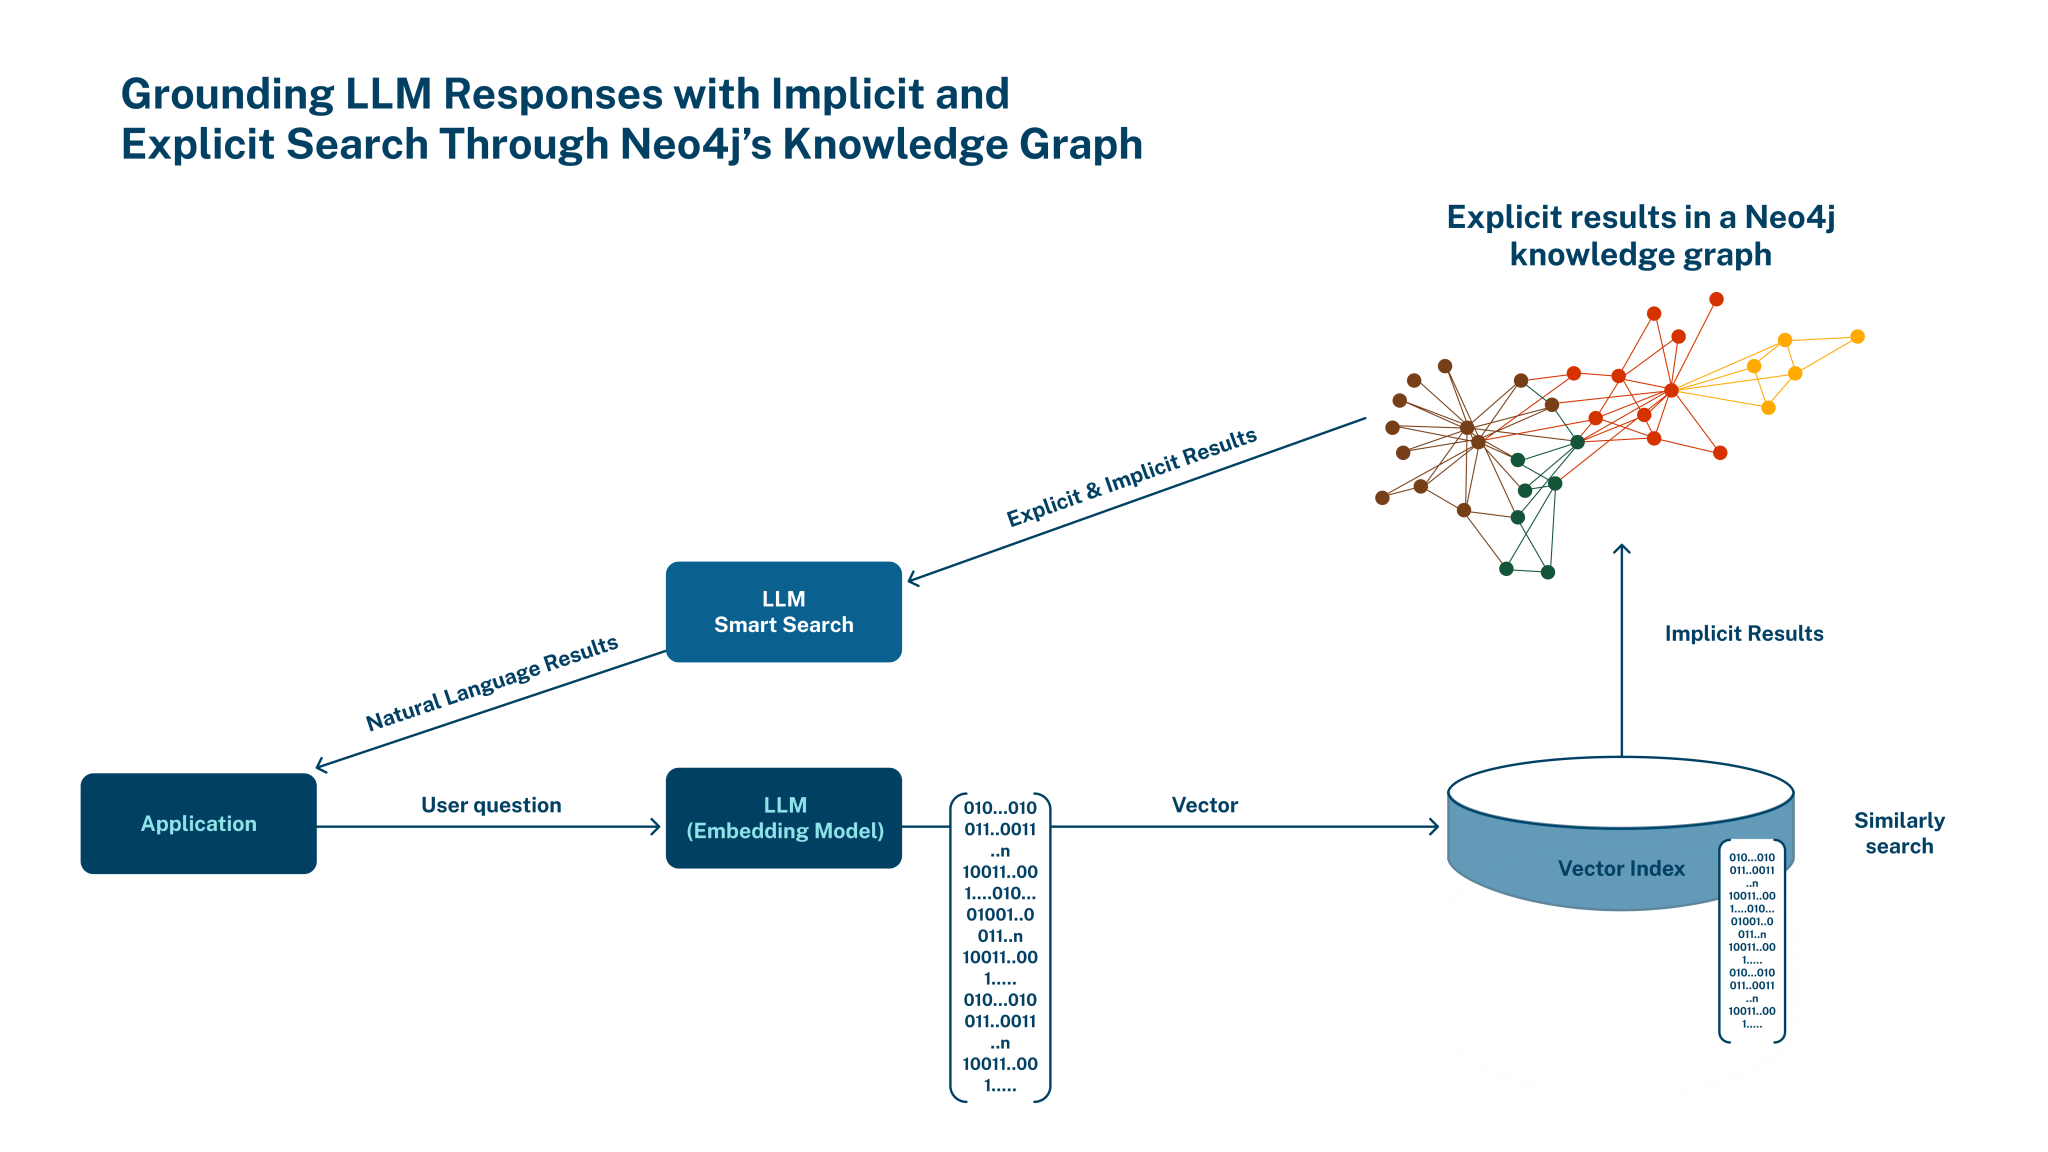
\includegraphics[width=4.86765in,height=2.74169in]{images/media/image23.png}

\begin{itemize}
\item
  Proses implementasi ini, parameter HNSW tidak dikonfigurasi secara
  eksplisit pada CREATE VECTOR INDEX (hanya vector.dimensions dan
  vector.similarity\_function yang dideklarasikan), sehingga Neo4j
  menerapkan nilai default:
\end{itemize}

\href{https://www.codecogs.com/eqnedit.php?latex=M\%20\%3D\%2016\%2C\%20\%5Cquad\%20\%5Ctext\%7Bef\%5C_construction\%7D\%20\%3D\%20100\#0}{
\includegraphics[width=2.36111in,height=0.15278in]{images/media/image16.png}}

Neo4j juga mengaktifkan vector quantization secara default untuk
mengoptimalkan penggunaan memori.

\begin{enumerate}
\def\labelenumi{\arabic{enumi}.}
\setcounter{enumi}{1}
\item
  \textbf{Candidate retrieval via ANN (Approximate Nearest Neighbor).}

  \begin{itemize}
  \item
    Untuk tiap query node q, dijalankan pencarian ANN pada Neo4j Vector
    Index yang mengembalikan top-k = 10 node terdekat berdasarkan cosine
    similarity. Cosine similarity antara dua vektor a dan b berdimensi d
    didefinisikan sebagai:
  \end{itemize}
\end{enumerate}

\href{https://www.codecogs.com/eqnedit.php?latex=\%5Ctext\%7Bsim\%7D(\%5Cmathbf\%7Ba\%7D\%2C\%20\%5Cmathbf\%7Bb\%7D)\%20\%3D\%20\%5Cfrac\%7B\%5Cmathbf\%7Ba\%7D\%20\%5Ccdot\%20\%5Cmathbf\%7Bb\%7D\%7D\%7B\%5C\%7C\%5Cmathbf\%7Ba\%7D\%5C\%7C\%20\%5Ctimes\%20\%5C\%7C\%5Cmathbf\%7Bb\%7D\%5C\%7C\%7D\%20\%3D\%20\%5Cfrac\%7B\%5Cdisplaystyle\%5Csum_\%7Bi\%3D1\%7D\%5E\%7Bd\%7D\%20a_i\%20\%5C\%2C\%20b_i\%7D\%7B\%5Csqrt\%7B\%5Cdisplaystyle\%5Csum_\%7Bi\%3D1\%7D\%5E\%7Bd\%7D\%20a_i\%5E2\%7D\%20\%5C\%3B\%5Ctimes\%5C\%3B\%20\%5Csqrt\%7B\%5Cdisplaystyle\%5Csum_\%7Bi\%3D1\%7D\%5E\%7Bd\%7D\%20b_i\%5E2\%7D\%7D\#0}{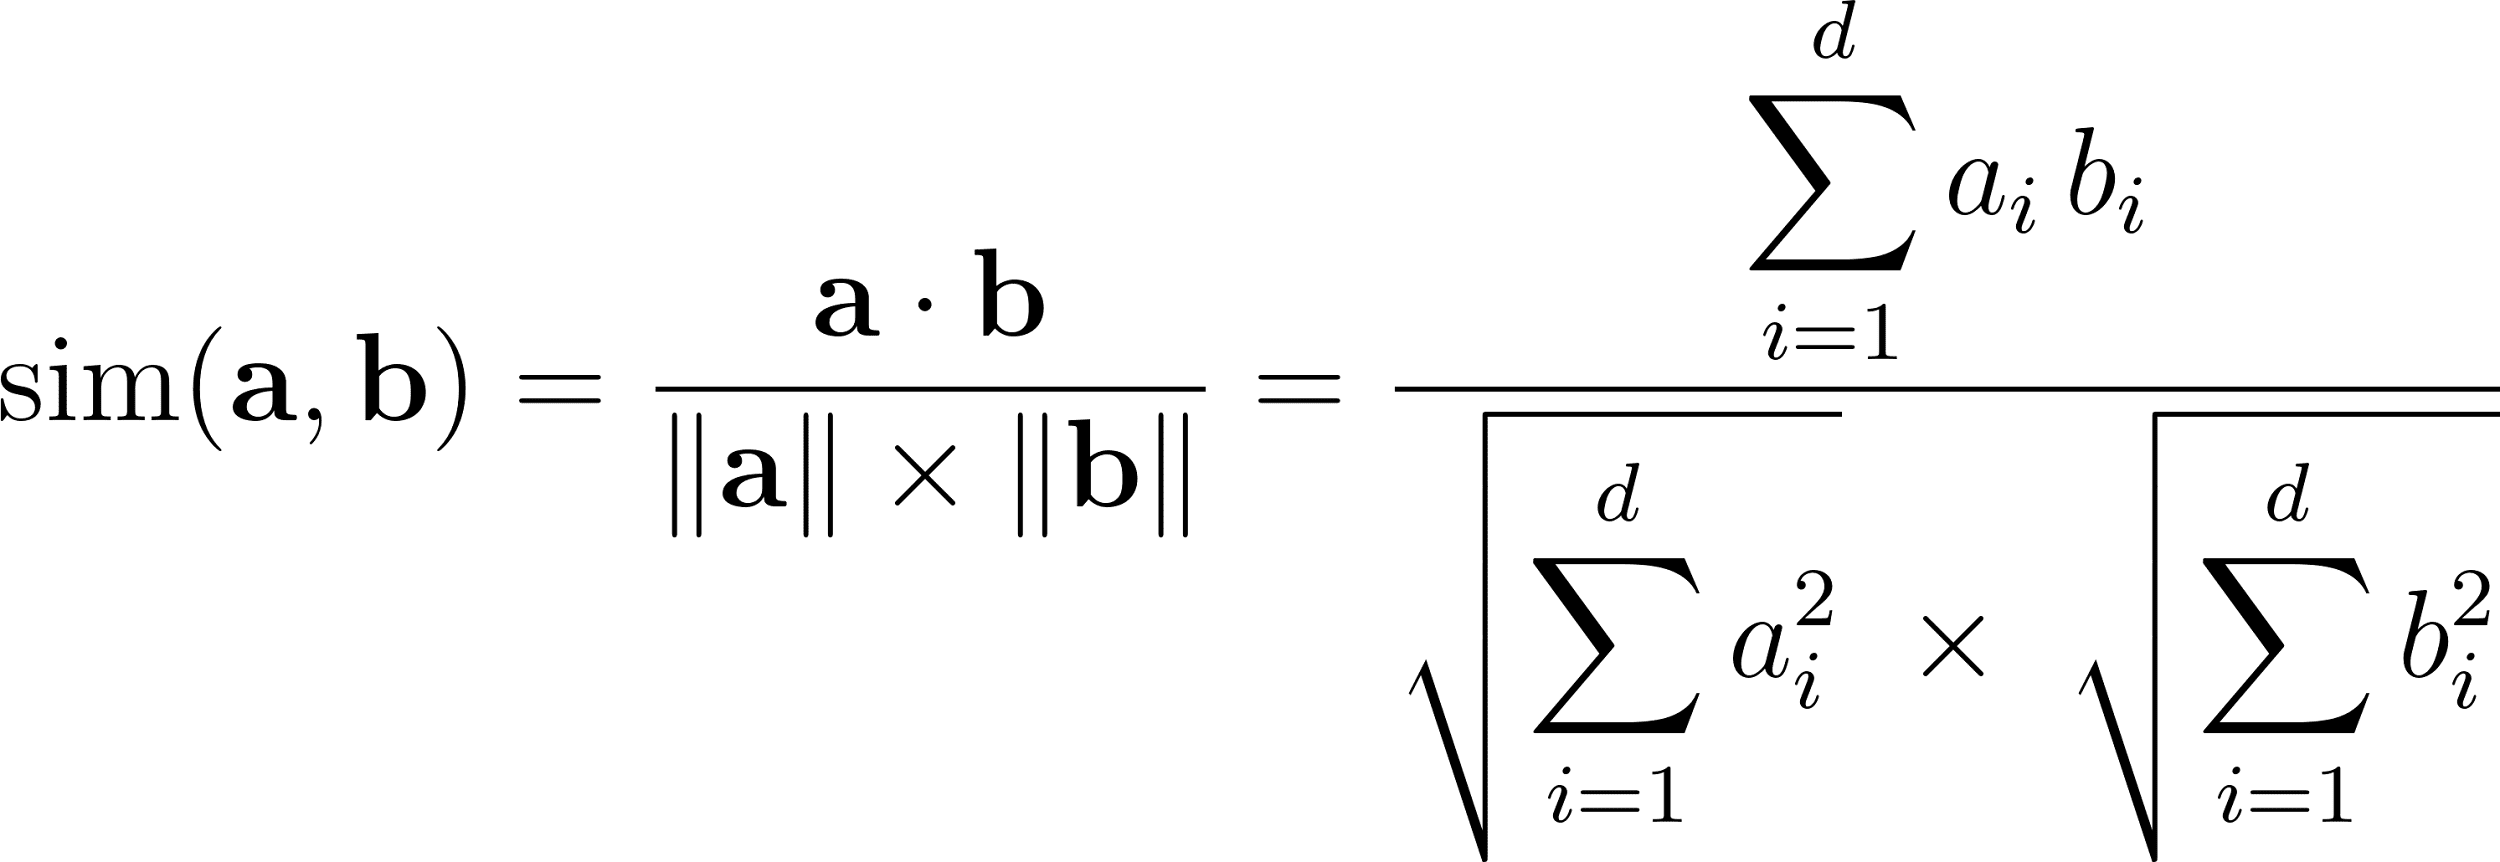
\includegraphics[width=3.16823in,height=1.08058in]{images/media/image25.png}}

\begin{itemize}
\item
  Nilai sim(a, b) berada dalam rentang {[}-1, 1{]}; nilai 1 menandakan
  vektor identik secara arah, 0 menandakan ortogonal (tidak berkaitan),
  dan -1 menandakan berlawanan arah. Pada konteks embedding teks, nilai
  cosine similarity umumnya berada dalam rentang {[}0, 1{]} karena semua
  komponen vektor cenderung non-negatif.
\end{itemize}

\href{https://www.codecogs.com/eqnedit.php?latex=\%5Ctext\%7Bsim\%7D(\%5Cmathbf\%7Ba\%7D\%2C\%20\%5Cmathbf\%7Bb\%7D)\%20\%5Cin\%20\%5B-1\%2C\%20\%5C\%3B\%201\%5D\#0}{
\includegraphics[width=1.34722in,height=0.16667in]{images/media/image18.png}}

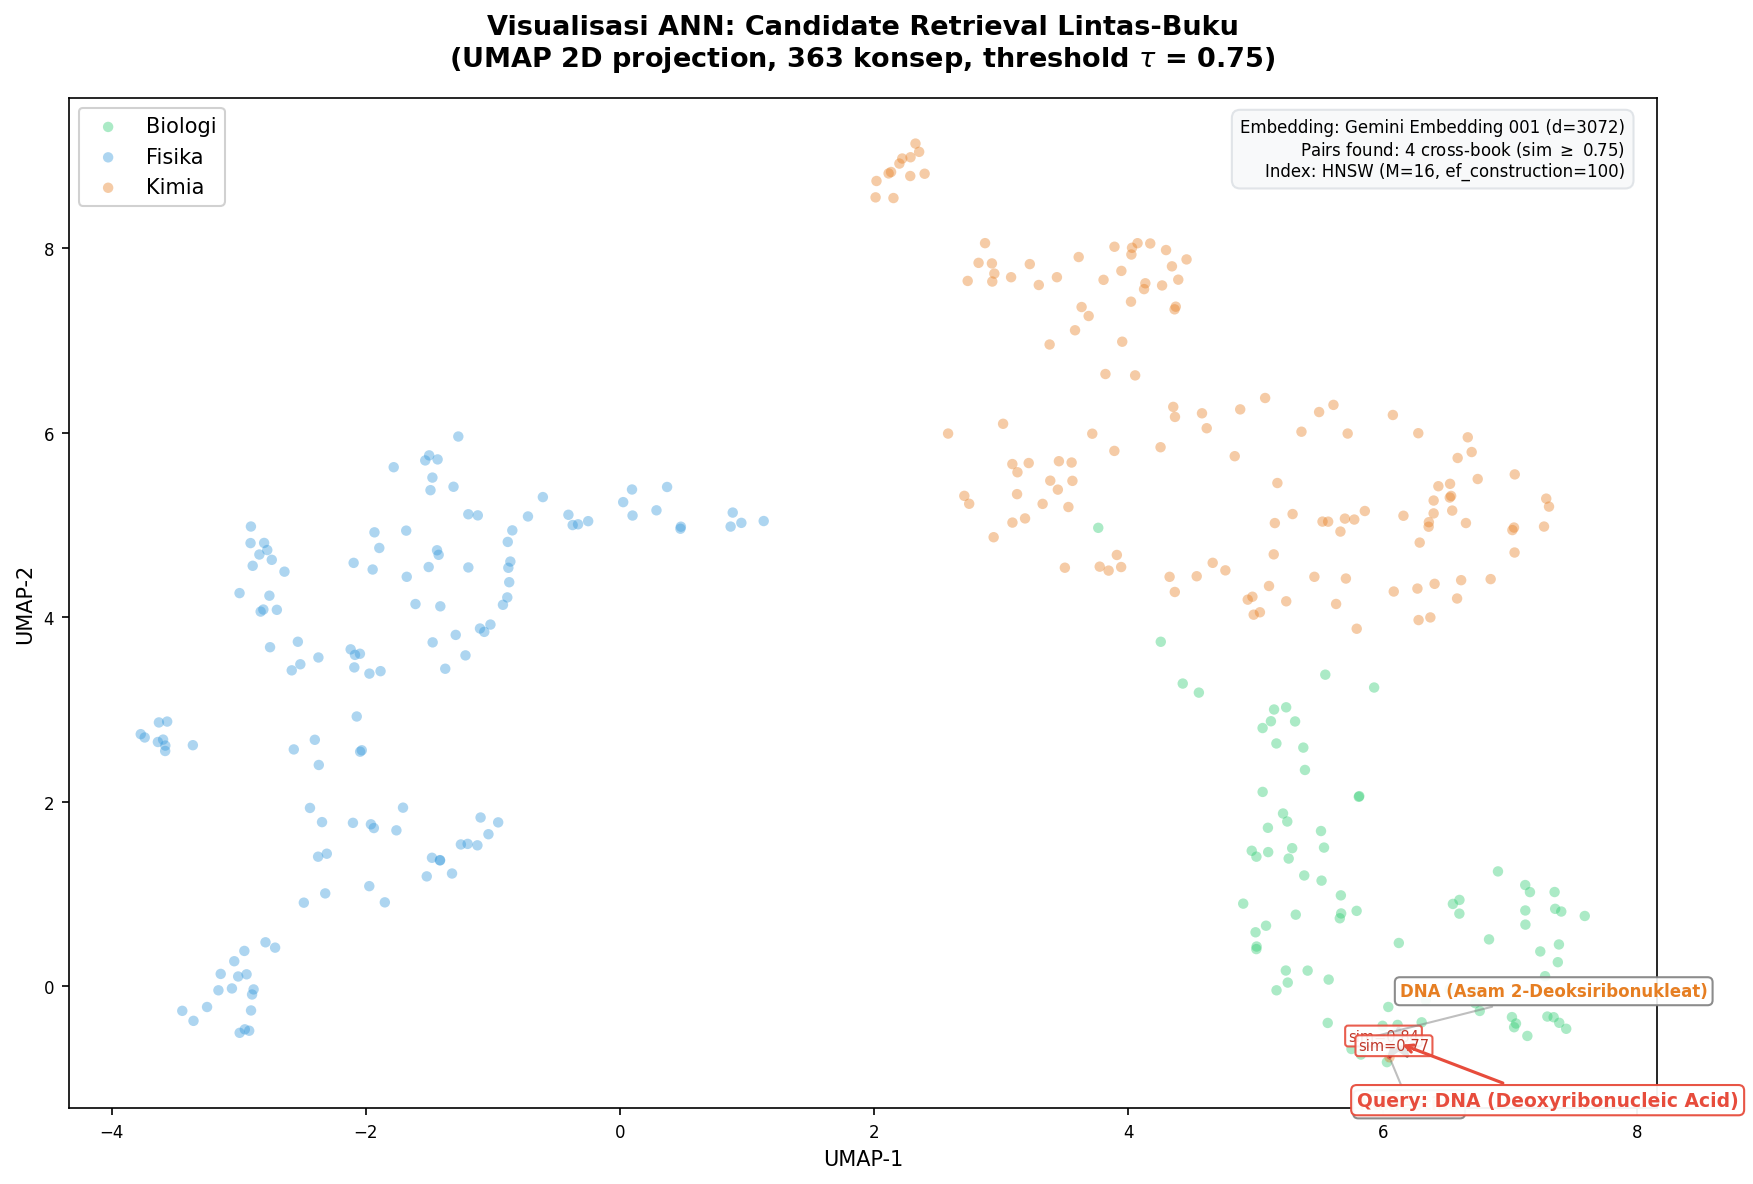
\includegraphics[width=5.51147in,height=3.72222in]{images/media/image5.png}

\begin{itemize}
\item
  Hanya pasangan dengan sim \textgreater= threshold yang lolos ke tahap
  berikutnya (threshold = 0.80 untuk pencarian intra-buku; threshold =
  0.75 untuk pencarian lintas-buku).
\end{itemize}

\href{https://www.codecogs.com/eqnedit.php?latex=\%5Ctext\%7Bcandidates\%7D(q)\%20\%3D\%20\%5Cleft\%5C\%7B\%20\%5C\%2C\%20c\%20\%5Cin\%20\%5Cmathcal\%7BC\%7D\%20\%5C\%3B\%5Cmiddle\%7C\%5C\%3B\%20\%5Ctext\%7Bsim\%7D(\%5Cmathbf\%7Be\%7D_q\%2C\%20\%5C\%2C\%20\%5Cmathbf\%7Be\%7D_c)\%20\%5Cgeq\%20\%5Ctau\%20\%5C\%2C\%20\%5Cright\%5C\%7D\#0}{
\includegraphics[width=3.04167in,height=0.16667in]{images/media/image20.png}}

\begin{itemize}
\item
  Pemakaian indeks vektor HNSW menurunkan kompleksitas total dari
  O(n\^{}2) pada perbandingan pairwise eksak menjadi O(n log n) untuk n
  konsep, sehingga pencarian relasi lintas-dokumen tetap tractable pada
  skala ratusan hingga ribuan konsep.
\end{itemize}

\begin{enumerate}
\def\labelenumi{\arabic{enumi}.}
\setcounter{enumi}{2}
\item
  \textbf{Candidate pruning.}

  \begin{itemize}
  \item
    Pasangan kandidat yang lolos ANN disaring melalui empat filter
    sebelum diklasifikasi LLM:

    \begin{enumerate}
    \def\labelenumii{\roman{enumii}.}
    \item
      Self-pair exclusion: parameter exclude\_name pada query ANN
      mencegah node menjadi kandidat dirinya sendiri.
    \item
      Deduplication: pasangan dinormalisasi sebagai tuple terurut
      sorted({[}A, B{]}) sehingga (A, B) dan (B, A) dianggap identik dan
      hanya diproses sekali.
    \item
      Cross-grade filter (khusus lintas-buku): pasangan dengan grade
      (mata pelajaran) yang sama dibuang, karena relasi within-subject
      sudah ditangani pada Tahap 2. Filter ini memastikan tahap
      completion hanya menemukan jembatan antar-disiplin ilmu.
    \item
      Existing typed edge filter: pasangan yang sudah memiliki edge
      bertipe selain SIMILAR\_TO dibuang agar tidak terjadi duplikasi
      relasi.
    \end{enumerate}
  \item
    Tahap pruning ini secara signifikan menekan jumlah pasangan yang
    diumpankan ke LLM, sehingga mengurangi biaya inferensi dan menjaga
    precision.
  \end{itemize}
\item
  \textbf{Relation classification via LLM.}

  \begin{itemize}
  \item
    Tiap pasangan yang lolos pruning diklasifikasikan oleh LLM (Gemini
    2.5 Flash) melalui prompt few-shot yang memuat: (1) deskripsi dan
    konteks kedua konsep (nama, deskripsi, mata pelajaran), (2) konteks
    graf (KONTEKS GRAF) berupa bab/chapter asal, hingga 5 existing
    out-edges, dan shared neighbors, serta (3) definisi ketat tiap label
    target.
  \item
    Untuk klasifikasi lintas-buku, LLM memilih salah satu dari lima
    label semantik:

    \begin{enumerate}
    \def\labelenumii{\roman{enumii}.}
    \item
      LINTAS\_BUKU\_SAMA\_DENGAN: A dan B merujuk pada entitas semantik
      yang sama lintas buku (simetris).
    \item
      LINTAS\_BUKU\_APLIKASI\_DARI: A adalah aplikasi/manifestasi konsep
      B di disiplin berbeda (asimetris).
    \item
      LINTAS\_BUKU\_PRASYARAT\_UNTUK: A pada satu mapel menjadi
      prasyarat untuk B di mapel lain (asimetris).
    \item
      LINTAS\_BUKU\_PRASYARAT\_UNTUK: A memperdalam/memperluas pemahaman
      B di buku lain (asimetris).
    \item
      LINTAS\_BUKU\_BERKAITAN\_DENGAN: A dan B berkaitan secara umum
      lintas buku tanpa struktur ketat (simetris, fallback).
    \item
      none: kemiripan semantik hanya superfisial; tidak ada relasi
      kurikuler bermakna.
    \end{enumerate}
  \item
    Klasifikasi dilengkapi skor confidence dalam rentang {[}0, 1{]}.
    Hasil klasifikasi di-cache menggunakan kunci order-invariant dengan
    fingerprint konteks graf (hash MD5 dari neighborhood), sehingga
    re-run setelah perubahan graf memicu re-klasifikasi otomatis.
  \end{itemize}
\end{enumerate}

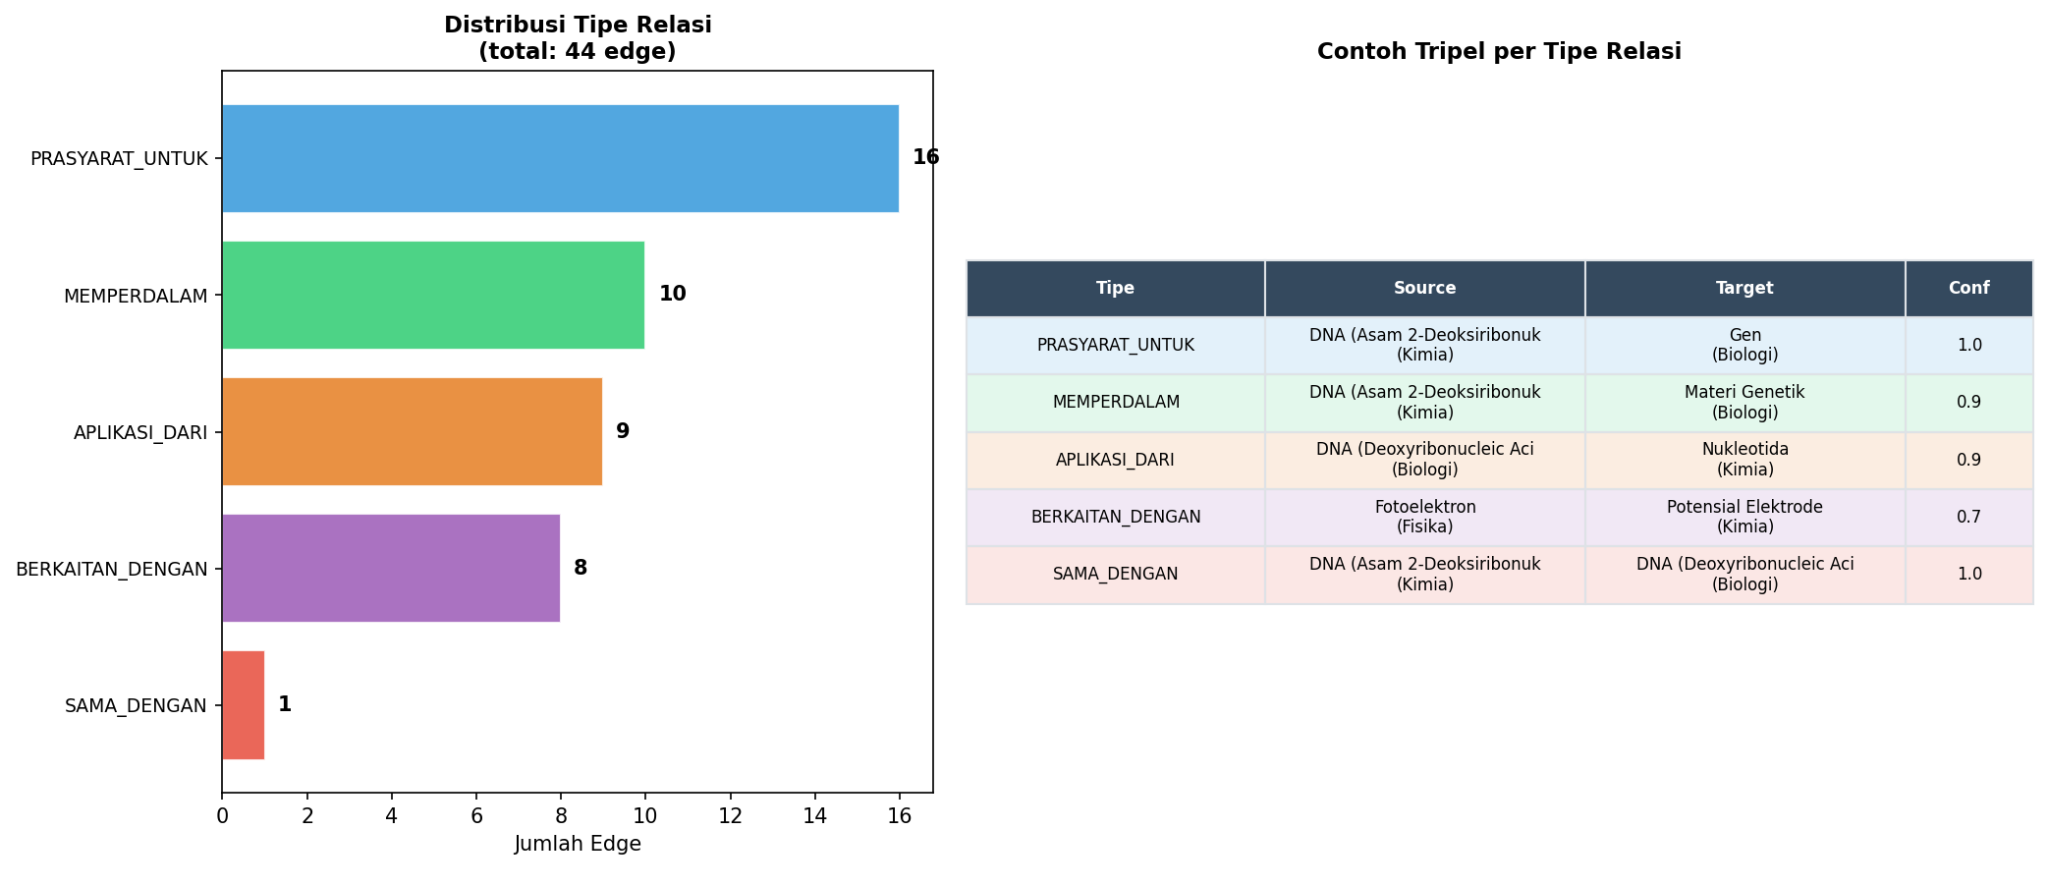
\includegraphics[width=5.51147in,height=2.33333in]{images/media/image22.png}

Distribusi tipe relasi hasil klasifikasi LLM beserta contoh triple per
tipe.

\begin{enumerate}
\def\labelenumi{\arabic{enumi}.}
\setcounter{enumi}{4}
\item
  \textbf{Edge writeback.}

  \begin{itemize}
  \item
    Hanya pasangan dengan label non-none yang dituliskan kembali sebagai
    edge baru ke Neo4j beserta properti confidence score, description
    (satu kalimat rationale Bahasa Indonesia), dan method (identifier
    model dan versi prompt). Strategi ini melengkapi graf tanpa menambah
    noise terstruktur, menghasilkan knowledge graph yang lebih lengkap
    secara topologis sambil menjaga kualitas relasi melalui gating LLM.
  \end{itemize}
\end{enumerate}

\textbf{4.1.5 Arsitektur Instrumen Evaluasi (KG Review App berbasis
Next.js/Redis)}

Untuk mengukur efektivitas dan kualitas Knowledge Graph (KG) yang telah
dibangun, penelitian ini mengembangkan instrumen evaluasi khusus yang
terdiri dari dua komponen arsitektur utama: kalkulasi metrik struktural
berbasis Cypher dan aplikasi web KG Review App untuk validasi pakar.

\begin{enumerate}
\def\labelenumi{\arabic{enumi}.}
\item
  \textbf{Implementasi Kalkulasi Struktural pada Neo4j Aura} Seluruh
  perhitungan metrik topologi graf dieksekusi secara langsung di sisi
  basis data menggunakan kueri \emph{Cypher} pada Neo4j Aura. Pendekatan
  eksekusi database-side ini memastikan bahwa metrik dapat diturunkan
  ulang setiap saat melalui kueri read-only. Pendekatan ini dirancang
  khusus agar kompatibel dengan spesifikasi tier Aura Free yang tidak
  menyertakan pustaka Graph Data Science (GDS), sehingga hasil
  perhitungannya dapat langsung diintegrasikan ke dalam dashboard
  visualisasi.
\item
  \textbf{Arsitektur KG Review App (Next.js dan Redis)} Untuk
  memfasilitasi evaluasi intrinsik oleh pakar (human evaluation),
  dikembangkan sebuah aplikasi web kustom bernama KG Review App. Dari
  sisi frontend, aplikasi ini dibangun menggunakan kerangka kerja
  Next.js berbasis React yang mendukung server-side rendering. Pada sisi
  backend, route handler Next.js dikonfigurasi untuk berkomunikasi
  secara asinkron dengan Redis yang bertindak sebagai primary key-value
  store.
\end{enumerate}

Penggunaan \emph{Redis} dipilih secara spesifik karena karakteristik
latensinya yang sangat rendah (low-latency read/write), menjadikannya
ideal untuk menangani payload ukuran kecil seperti rating per-triple dan
fitur auto-save. Model persistensi data (persistence model) pada
aplikasi ini dirancang sedemikian rupa sehingga setiap aksi penilaian
(rating) dari pakar akan memicu debounced auto-save ke Redis. Skema
kunci (key) yang digunakan berformat
expert:\{expert\_id\}:\{mapel\}:\{triple\_id\} yang memetakan nilai ke
dalam objek JSON \{label, comment, timestamp\}. Skema Key-Value (KV) ini
sangat efisien karena memungkinkan reviewer untuk melanjutkan sesi
peninjauan (resume) tanpa memerlukan arsitektur relasional yang kompleks
(transaksi multi-tabel), sekaligus mempermudah proses ekspor feedback
JSON yang nantinya diumpankan kembali ke LLM.

Gambar 4.x Antarmuka Halaman Login KG Review App.

\begin{enumerate}
\def\labelenumi{\arabic{enumi}.}
\setcounter{enumi}{2}
\item
  \textbf{Role-Based Access Control (RBAC)} Untuk menjaga integritas
  proses validasi, arsitektur aplikasi menerapkan kontrol akses berbasis
  peran (RBAC) dengan dua peran utama:

  \begin{enumerate}
  \def\labelenumii{\alph{enumii}.}
  \item
    Admin: Memiliki hak akses manajerial untuk mengunggah berkas JSON
    hasil ekstraksi (Tahap 3 dan 4) ke dalam sistem per mata pelajaran,
    mengatur status publikasi graf, serta melihat panel metrik (tinjauan
    respons) dari para pakar dalam mode read-only.
  \item
    Expert (Reviewer): Memiliki hak akses read-write operasional untuk
    memberikan rating pada setiap triple relasi yang disajikan, serta
    memberikan masukan jika ada triple esensial yang hilang (missing
    triples) melalui form penambahan.
  \end{enumerate}
\end{enumerate}

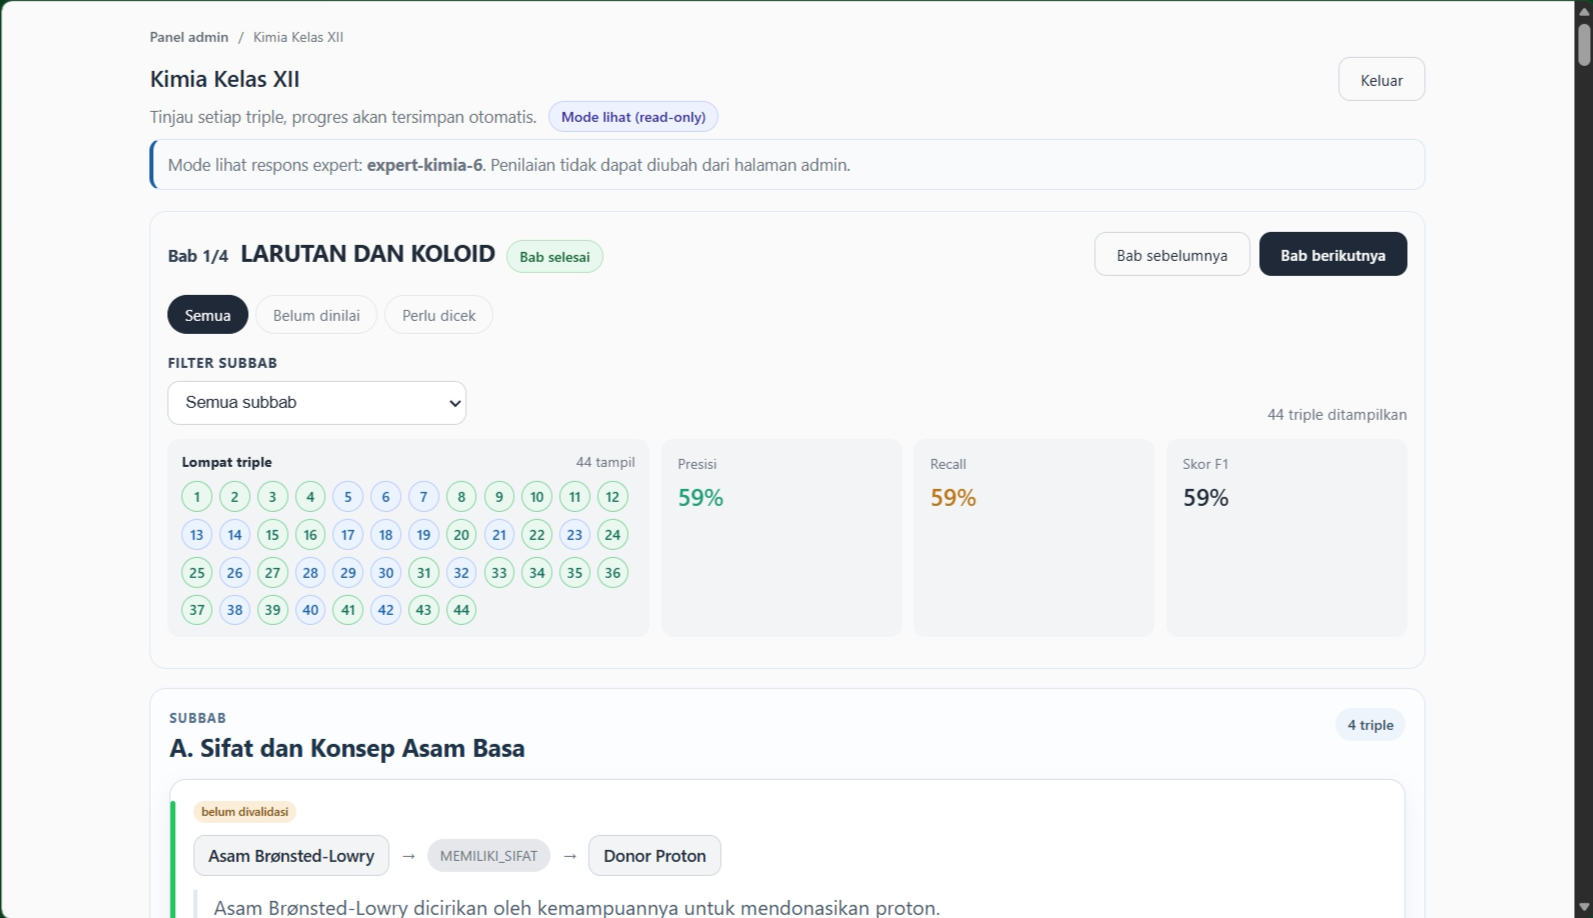
\includegraphics[width=5.51147in,height=3.18056in]{images/media/image13.png}

Gambar 4.x Tampilan Dasbor Admin untuk mengunggah graf JSON.

Gambar 4.x Antarmuka Admin untuk memantau progres review pakar.

\begin{enumerate}
\def\labelenumi{\arabic{enumi}.}
\setcounter{enumi}{3}
\item
  \textbf{Desain Skema Validasi Dua Fase} Mengingat kompleksitas
  ontologi kurikulum sains, antarmuka evaluasi untuk Expert dirancang
  menggunakan skema studi dua fase guna menurunkan beban kognitif
  (cognitive load) penilai:

  \begin{enumerate}
  \def\labelenumii{\alph{enumii}.}
  \item
    \textbf{Fase 1 (Validasi Intra-Mapel):} Pakar mengevaluasi kualitas
    hierarki dan relasi semantik secara spesifik di dalam lingkup satu
    mata pelajaran (misalnya Fisika saja).
  \item
    \textbf{Fase 2 (Interkoneksi Antar-Mapel):} Pakar secara khusus
    mengevaluasi validitas relasi implisit lintas-disiplin sains
    (berlabel LINTAS\_BUKU\_*) yang diprediksi oleh LLM pada tahap
    completion. Pemisahan fase ini memungkinkan analisis data yang lebih
    terisolasi dan akurat.
  \end{enumerate}
\end{enumerate}

\textbf{4.2 Hasil Evaluasi dan Pembahasan}

Tahap evaluasi dalam kerangka \emph{Design Science Research} (DSR) ini
bertujuan untuk mengukur performa dan kualitas \emph{Knowledge Graph}
(KG) yang dihasilkan oleh pipeline sistem. Evaluasi dilakukan secara
komprehensif melalui analisis kuantitatif terhadap topologi graf,
validasi kualitatif oleh pakar domain, pembahasan mendalam terkait
\emph{error} model LLM, serta komparasi antar-disiplin ilmu sains.

\textbf{4.2.1 Hasil Analisis Struktural Graf}

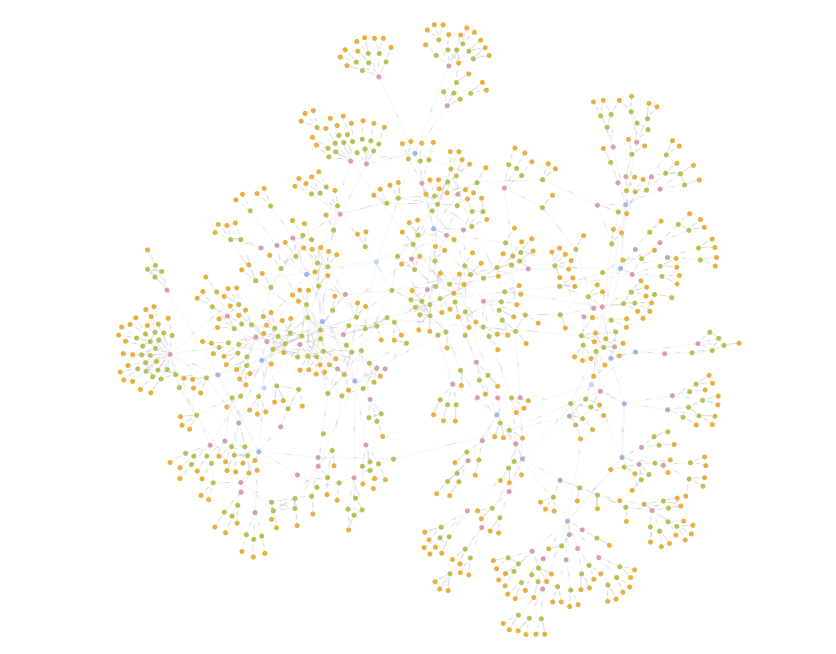
\includegraphics[width=5.51147in,height=4.30556in]{images/media/image21.png}

Gambar 4.x --- Visualisasi topologi keseluruhan knowledge graph hasil
konstruksi

Analisis struktural bertujuan untuk mengevaluasi kualitas interkoneksi
jaringan pengetahuan secara matematis, khususnya untuk melihat
perbandingan struktur graf sebelum Knowledge Graph Completion (pre-KGC)
dan sesudahnya (post-KGC). Seluruh perhitungan pada bagian ini
dieksekusi melalui kueri Cypher di Neo4j dengan berpedoman pada
formulasi metrik topologi yang telah dijelaskan pada \textbf{Subbab
2.2.1}.

\begin{longtable}[]{@{}
  >{\raggedright\arraybackslash}p{(\columnwidth - 4\tabcolsep) * \real{0.2476}}
  >{\raggedright\arraybackslash}p{(\columnwidth - 4\tabcolsep) * \real{0.3306}}
  >{\raggedright\arraybackslash}p{(\columnwidth - 4\tabcolsep) * \real{0.4218}}@{}}
\toprule()
\begin{minipage}[b]{\linewidth}\raggedright
\textbf{Metrik Struktural}
\end{minipage} & \begin{minipage}[b]{\linewidth}\raggedright
\textbf{Pre-KGC (Siloed Graph)}
\end{minipage} & \begin{minipage}[b]{\linewidth}\raggedright
\textbf{Post-KGC (Integrated Graph)}
\end{minipage} \\
\begin{minipage}[b]{\linewidth}\raggedright
ADC
\end{minipage} & \begin{minipage}[b]{\linewidth}\raggedright
{[}Pre{]}
\end{minipage} & \begin{minipage}[b]{\linewidth}\raggedright
{[}Post{]}
\end{minipage} \\
\begin{minipage}[b]{\linewidth}\raggedright
Graph Density
\end{minipage} & \begin{minipage}[b]{\linewidth}\raggedright
{[}Pre{]}
\end{minipage} & \begin{minipage}[b]{\linewidth}\raggedright
{[}Post{]}
\end{minipage} \\
\begin{minipage}[b]{\linewidth}\raggedright
Modularity
\end{minipage} & \begin{minipage}[b]{\linewidth}\raggedright
{[}Pre{]}
\end{minipage} & \begin{minipage}[b]{\linewidth}\raggedright
{[}Post{]}
\end{minipage} \\
\midrule()
\endhead
\bottomrule()
\end{longtable}

\begin{enumerate}
\def\labelenumi{\arabic{enumi}.}
\item
  \begin{quote}
  \textbf{Evaluasi \emph{Average Degree Centrality} (ADC) dan Kepadatan
  (Density)} Berdasarkan \textbf{Tabel 4.X}, terjadi peningkatan nilai
  ADC dari {[}Nilai Pre-KGC{]} menjadi {[}Nilai Post-KGC{]} pada fase
  post-KGC. {[}proceed{]}
  \end{quote}
\item
  \begin{quote}
  \textbf{Evaluasi \emph{Modularity}} Analisis struktur komunitas
  menggunakan metrik \emph{Modularity} pada fase Pre-KGC mencatatkan
  nilai global yang sangat tinggi ({[}Nilai Pre-KGC{]}).
  \end{quote}
\item
  \begin{quote}
  \textbf{Evaluasi Metrik Ekstraksi dan Hubungan} Di luar evaluasi
  topologi di atas, kualitas hasil ekstraksi LLM secara spesifik diukur
  menggunakan metrik \emph{Description Completeness} dan \emph{Typed
  Relation Ratio} (TRR) sebagaimana didefinisikan pada \textbf{Subbab
  2.2.2} dan \textbf{2.2.3}. Sistem mencatatkan nilai kelengkapan
  deskripsi sebesar {[}Nilai DC{]}\% dan rasio instansiasi relasi
  semantik spesifik sebesar {[}Nilai TRR{]}\%, {[}proceed{]}
  \end{quote}
\end{enumerate}

\textbf{4.2.2 Hasil Validasi Pakar (Expert Validation)}

Evaluasi performa sistem dalam mengekstrak dan memprediksi relasi
dievaluasi langsung oleh panel pakar (sebanyak 6 reviewer) menggunakan
instrumen KG Review App. Berdasarkan desain studi dua fase, hasil
evaluasi dipisahkan menjadi evaluasi intra-mapel dan inter-mapel. Data
dianalisis menggunakan metrik \emph{Precision, Recall, F1-Score}, dan
uji kesepakatan AC1 yang merujuk pada \textbf{Subbab 2.2.4}.

\begin{longtable}[]{@{}
  >{\raggedright\arraybackslash}p{(\columnwidth - 6\tabcolsep) * \real{0.2576}}
  >{\raggedright\arraybackslash}p{(\columnwidth - 6\tabcolsep) * \real{0.2273}}
  >{\raggedright\arraybackslash}p{(\columnwidth - 6\tabcolsep) * \real{0.2727}}
  >{\raggedright\arraybackslash}p{(\columnwidth - 6\tabcolsep) * \real{0.2424}}@{}}
\toprule()
\begin{minipage}[b]{\linewidth}\raggedright
\textbf{Mata Pelajaran}
\end{minipage} & \begin{minipage}[b]{\linewidth}\raggedright
\textbf{Reviewer 1}
\end{minipage} & \begin{minipage}[b]{\linewidth}\raggedright
\textbf{Reviewer 2}
\end{minipage} & \begin{minipage}[b]{\linewidth}\raggedright
\textbf{Final}
\end{minipage} \\
\begin{minipage}[b]{\linewidth}\raggedright
Fisika
\end{minipage} & \begin{minipage}[b]{\linewidth}\raggedright
\end{minipage} & \begin{minipage}[b]{\linewidth}\raggedright
\end{minipage} & \begin{minipage}[b]{\linewidth}\raggedright
\end{minipage} \\
\begin{minipage}[b]{\linewidth}\raggedright
Kimia
\end{minipage} & \begin{minipage}[b]{\linewidth}\raggedright
\end{minipage} & \begin{minipage}[b]{\linewidth}\raggedright
\end{minipage} & \begin{minipage}[b]{\linewidth}\raggedright
\end{minipage} \\
\begin{minipage}[b]{\linewidth}\raggedright
Biologi
\end{minipage} & \begin{minipage}[b]{\linewidth}\raggedright
\end{minipage} & \begin{minipage}[b]{\linewidth}\raggedright
\end{minipage} & \begin{minipage}[b]{\linewidth}\raggedright
\end{minipage} \\
\midrule()
\endhead
\bottomrule()
\end{longtable}

\begin{longtable}[]{@{}
  >{\raggedright\arraybackslash}p{(\columnwidth - 8\tabcolsep) * \real{0.1928}}
  >{\raggedright\arraybackslash}p{(\columnwidth - 8\tabcolsep) * \real{0.1947}}
  >{\raggedright\arraybackslash}p{(\columnwidth - 8\tabcolsep) * \real{0.1815}}
  >{\raggedright\arraybackslash}p{(\columnwidth - 8\tabcolsep) * \real{0.1928}}
  >{\raggedright\arraybackslash}p{(\columnwidth - 8\tabcolsep) * \real{0.2382}}@{}}
\toprule()
\begin{minipage}[b]{\linewidth}\raggedright
\textbf{Fase Evaluasi}
\end{minipage} & \begin{minipage}[b]{\linewidth}\raggedright
\textbf{Expert 1}
\end{minipage} & \begin{minipage}[b]{\linewidth}\raggedright
\textbf{Recall}
\end{minipage} & \begin{minipage}[b]{\linewidth}\raggedright
\textbf{F1-Score}
\end{minipage} & \begin{minipage}[b]{\linewidth}\raggedright
\textbf{Skor Kesepakatan}
\end{minipage} \\
\begin{minipage}[b]{\linewidth}\raggedright
Fase 1
\end{minipage} & \begin{minipage}[b]{\linewidth}\raggedright
{[}Nilai P{]}
\end{minipage} & \begin{minipage}[b]{\linewidth}\raggedright
{[}Nilai R{]}
\end{minipage} & \begin{minipage}[b]{\linewidth}\raggedright
{[}Nilai F1{]}
\end{minipage} & \begin{minipage}[b]{\linewidth}\raggedright
\end{minipage} \\
\begin{minipage}[b]{\linewidth}\raggedright
Fase 2
\end{minipage} & \begin{minipage}[b]{\linewidth}\raggedright
{[}Nilai P{]}
\end{minipage} & \begin{minipage}[b]{\linewidth}\raggedright
{[}Nilai R{]}
\end{minipage} & \begin{minipage}[b]{\linewidth}\raggedright
{[}Nilai F1{]}
\end{minipage} & \begin{minipage}[b]{\linewidth}\raggedright
\end{minipage} \\
\midrule()
\endhead
\bottomrule()
\end{longtable}

\begin{enumerate}
\def\labelenumi{\arabic{enumi}.}
\item
  \textbf{Kuantitas Akurasi (Precision, Recall, F1-Score)} Secara
  agregat, presisi pada Fase 1 mencapai {[}Nilai Presisi Fase 1{]}\%,
  menunjukkan kemampuan dasar LLM yang sangat baik dalam memahami teks
  tunggal. Namun, pada Fase 2, presisi berada pada angka {[}Nilai
  Presisi Fase 2{]}\%. Perbandingan ini mengindikasikan bahwa LLM
  {[}misal, sangat pintar membaca teks tunggal, tetapi mengalami
  penurunan akurasi / memaksakan kecocokan saat ditugaskan menalar
  jembatan lintas ilmu sains{]}. Terdapat selisih antara Precision dan
  Recall sebesar {[}Nilai Selisih{]}\% akibat tingginya \emph{missing
  triples} yang ditambahkan pakar, menandakan sistem masih luput
  mengekstrak relasi esensial tertentu.
\item
  \textbf{Uji Kesepakatan Pakar (Inter-rater Reliability)} Sesuai dengan
  karakteristik relasi yang dinilai, Fase 1 menggunakan AC1
  {[}Proceed{]}
\end{enumerate}

\textbf{4.2.3 Pembahasan Kualitatif Hasil KGC}

Bagian ini membahas secara kualitatif kualitas relasi lintas-buku yang
ditemukan oleh pipeline Graph Completion, menganalisis pola kesalahan
model LLM, dan mengidentifikasi faktor-faktor yang memengaruhi akurasi
ekstraksi.

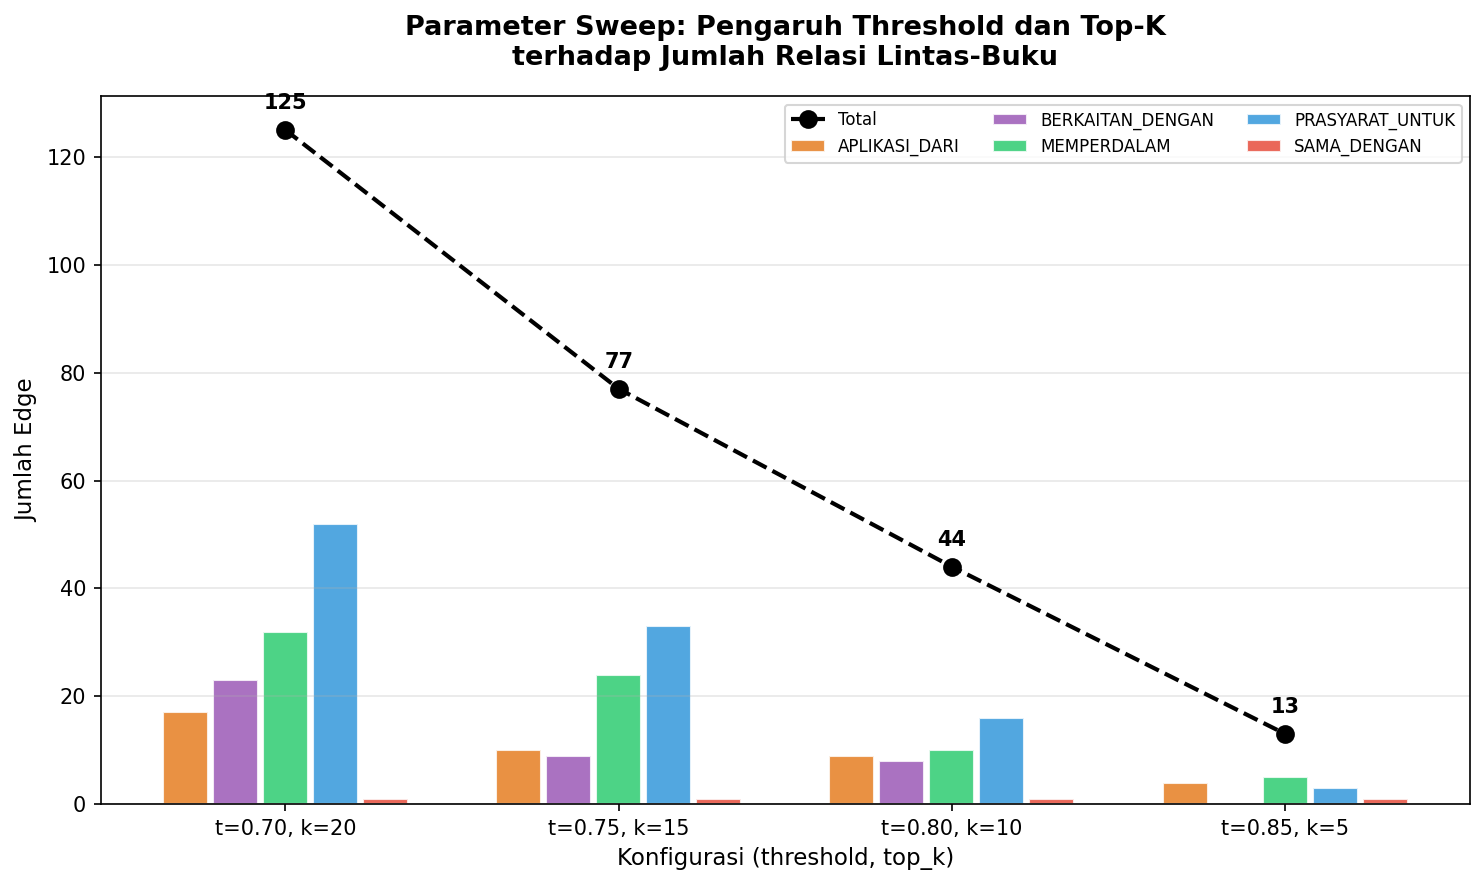
\includegraphics[width=5.51147in,height=3.29167in]{images/media/image3.png}

Parameter sweep: pengaruh threshold dan top-k terhadap jumlah relasi
lintas-buku yang ditemukan.

Pengaruh parameter retrieval terhadap jumlah relasi lintas-buku yang
ditemukan dievaluasi pada empat konfigurasi berpasangan, di mana ambang
kemiripan (\emph{threshold}) dinaikkan seiring penurunan jumlah tetangga
per node (\emph{top-k}). Semakin ketat konfigurasi, semakin sedikit
pasangan kandidat yang lolos: dari 101 relasi pada konfigurasi paling
permisif (0,70 / k20) menyusut menjadi hanya 14 relasi pada konfigurasi
paling ketat (0,85 / k5).

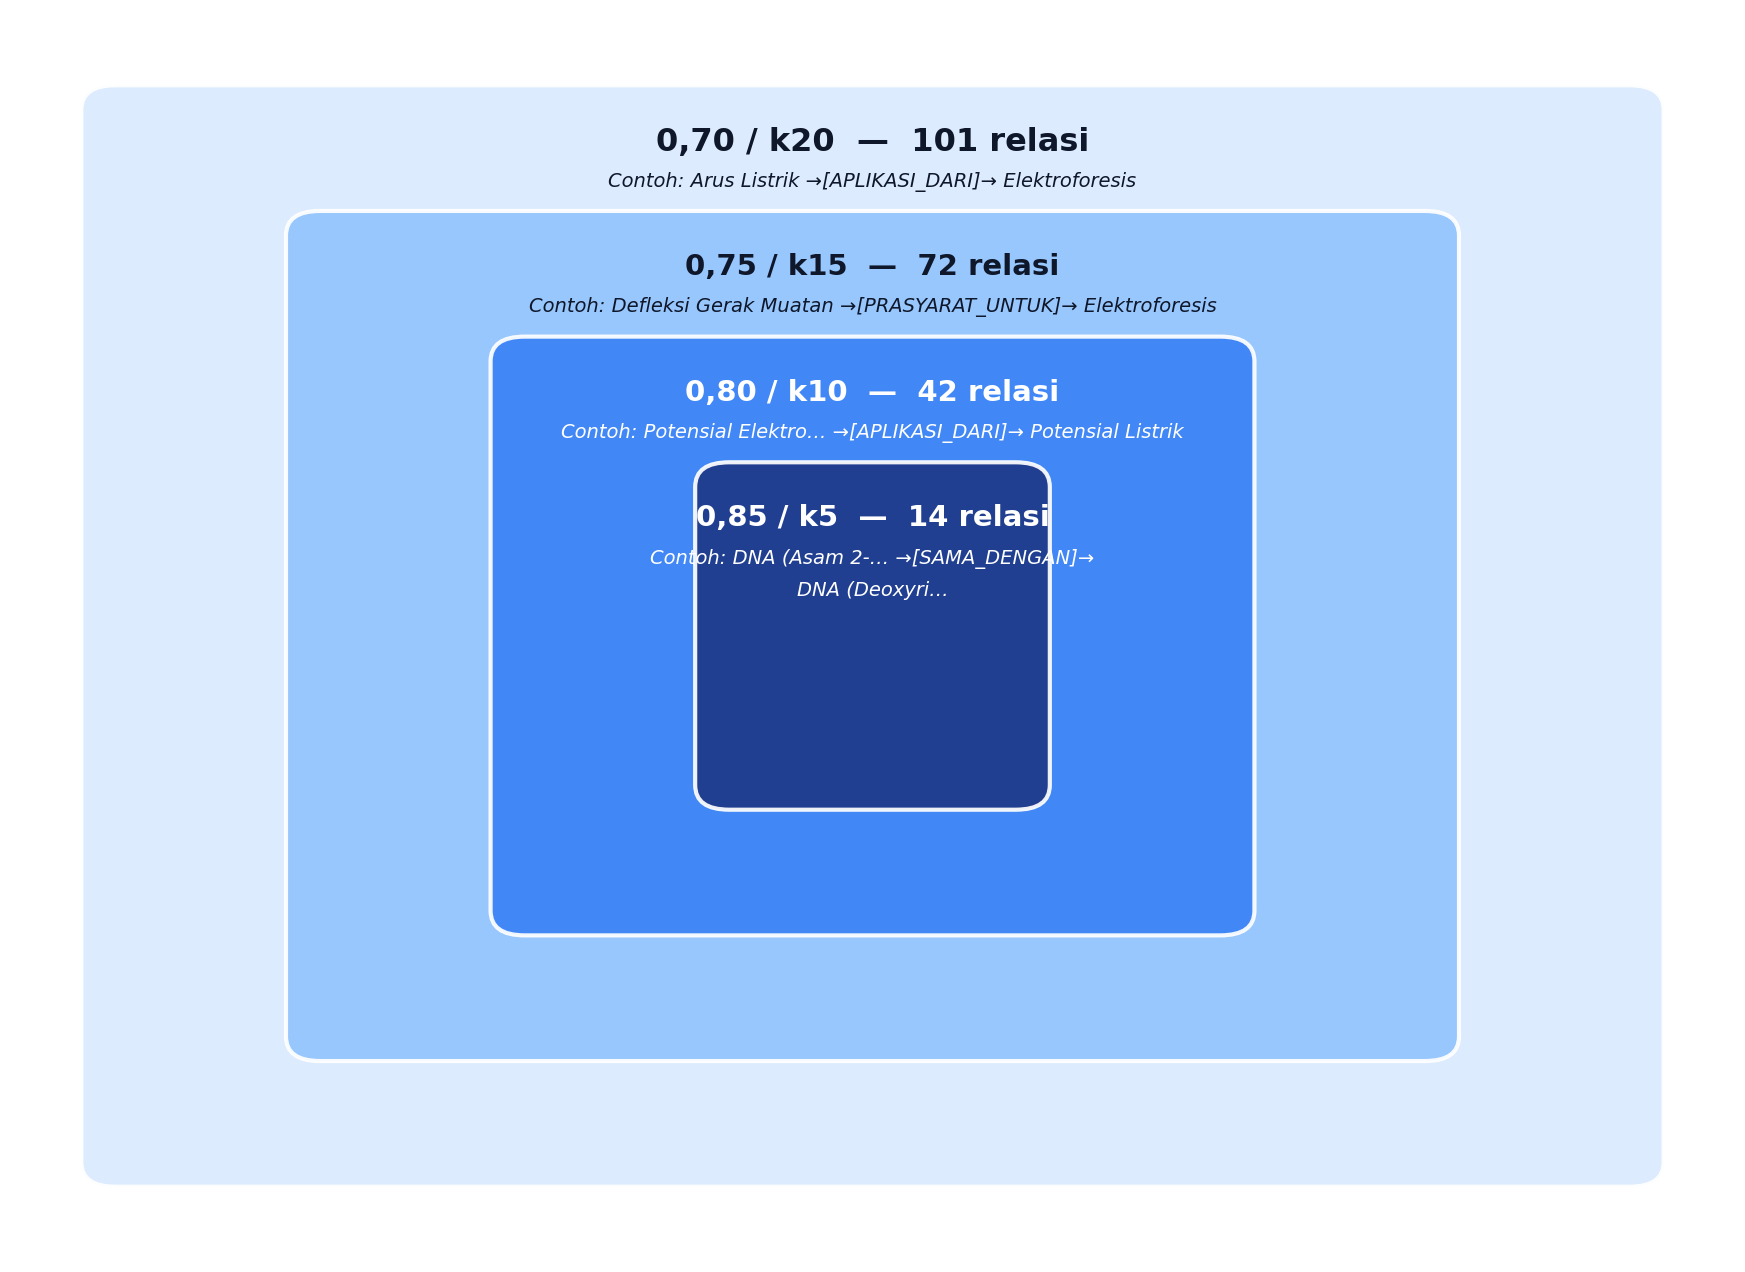
\includegraphics[width=5.02292in,height=3.56667in]{images/media/image4.png}

\textbf{Gambar 4.x} Struktur bersarang (nested) hasil \emph{parameter
sweep} relasi lintas-buku. Setiap konfigurasi yang lebih ketat
(threshold lebih tinggi, top-k lebih kecil) merupakan himpunan bagian
(\emph{subset}) dari konfigurasi yang lebih permisif

\begin{longtable}[]{@{}
  >{\raggedright\arraybackslash}p{(\columnwidth - 2\tabcolsep) * \real{0.3409}}
  >{\raggedright\arraybackslash}p{(\columnwidth - 2\tabcolsep) * \real{0.6591}}@{}}
\toprule()
\begin{minipage}[b]{\linewidth}\raggedright
\textbf{Konfigurasi (threshold / top-k)}
\end{minipage} & \begin{minipage}[b]{\linewidth}\raggedright
\textbf{Jumlah relasi}
\end{minipage} \\
\begin{minipage}[b]{\linewidth}\raggedright
0,70 / k20 (permisif --- konfigurasi final saat ini)
\end{minipage} & \begin{minipage}[b]{\linewidth}\raggedright
101
\end{minipage} \\
\begin{minipage}[b]{\linewidth}\raggedright
0,75 / k15
\end{minipage} & \begin{minipage}[b]{\linewidth}\raggedright
72
\end{minipage} \\
\begin{minipage}[b]{\linewidth}\raggedright
0,80 / k10
\end{minipage} & \begin{minipage}[b]{\linewidth}\raggedright
42
\end{minipage} \\
\begin{minipage}[b]{\linewidth}\raggedright
0,85 / k5 (paling ketat)
\end{minipage} & \begin{minipage}[b]{\linewidth}\raggedright
14
\end{minipage} \\
\midrule()
\endhead
\bottomrule()
\end{longtable}

Konfigurasi membentuk himpunan bersarang: setiap konfigurasi yang lebih
ketat merupakan himpunan bagian dari yang lebih permisif. Pengetatan
parameter dengan demikian berfungsi sebagai kompromi \emph{recall} ---
menukar cakupan relasi (lebih banyak interkoneksi ditemukan) dengan
selektivitas (hanya pasangan berkemiripan tertinggi yang dipertahankan).

Sebagaimana dibahas pada Subbab 4.2.3.1, pengetatan ini menurunkan
kuantitas relasi tetapi \textbf{tidak} memperbaiki ketepatan arah
relasi, yang tetap berkisar \textasciitilde74\% di seluruh rentang
0,70--0,80; artinya kesalahan arah tersebar merata pada seluruh rentang
kemiripan dan bukan persoalan yang dapat diselesaikan dengan penyetelan
\emph{threshold}.

\hypertarget{kualitas-relasi-lintas-buku-yang-ditemukan}{%
\paragraph{4.2.3.1 Kualitas Relasi Lintas-Buku yang
Ditemukan}\label{kualitas-relasi-lintas-buku-yang-ditemukan}}

Paada konfigurasi final (threshold = 0,70; top\_k = 20; scope
lintas-mapel), pipeline menemukan 125 relasi lintas-buku. Distribusi
tipe relasi didominasi PRASYARAT\_UNTUK (57 edge, 45,6\%), diikuti
MEMPERDALAM (31 edge, 24,8\%), BERKAITAN\_DENGAN (21 edge, 16,8\%),
APLIKASI\_DARI (15 edge, 12,0\%), dan SAMA\_DENGAN (1 edge, 0,8\%).
Dominasi PRASYARAT\_UNTUK mengindikasikan bahwa jembatan lintas-disiplin
pada kurikulum sains kelas XII lebih banyak bersifat prasyarat
pengetahuan daripada aplikasi atau analogi. Dari 125 relasi, 8 edge
berkonfidens \textless{} 0,5 (seluruhnya BERKAITAN\_DENGAN) dikeluarkan
dari survei validasi utama, menyisakan 117 relasi yang dinilai pakar.

Dari 125 edge, 20 (16\%) memiliki skor confidence = 1,0, menunjukkan
keyakinan tinggi LLM terhadap relasi tersebut.. Contoh relasi dengan
confidence tertinggi meliputi:

\begin{itemize}
\item
  \begin{quote}
  DNA (Asam 2-Deoksiribonukleat) {[}Kimia{]} → Gen {[}Biologi{]}:
  PRASYARAT\_UNTUK (conf = 1.0). Pemahaman struktur kimia DNA merupakan
  fondasi untuk memahami fungsi gen secara biologis.
  \end{quote}
\item
  \begin{quote}
  Potensial Elektrode {[}Kimia{]} → Potensial Listrik {[}Fisika{]}:
  APLIKASI\_DARI (conf = 1.0). Konsep potensial elektrode dalam
  elektrokimia merupakan aplikasi langsung dari konsep potensial listrik
  dalam fisika.
  \end{quote}
\item
  \begin{quote}
  Enzim {[}Biologi{]} → Protein {[}Kimia{]}: APLIKASI\_DARI (conf =
  1.0). Enzim merupakan manifestasi fungsional dari protein dalam
  konteks biologis.
  \end{quote}
\item
  \begin{quote}
  Fosforilasi Oksidatif {[}Biologi{]} → Oksidasi {[}Kimia{]}:
  PRASYARAT\_UNTUK (conf = 1.0). Pemahaman reaksi oksidasi secara kimia
  diperlukan sebelum mempelajari fosforilasi oksidatif dalam
  metabolisme.
  \end{quote}
\end{itemize}

Satu-satunya relasi bertipe SAMA\_DENGAN yang ditemukan adalah DNA (Asam
2-Deoksiribonukleat) {[}Kimia{]} ↔ DNA (Deoxyribonucleic Acid)
{[}Biologi{]} dengan confidence 1.0. Temuan ini mengonfirmasi bahwa
pipeline mampu mendeteksi entitas identik yang diajarkan di dua disiplin
berbeda dengan terminologi yang sedikit berbeda.

\textbf{Validasi Pakar atas Relasi Lintas-Buku}

Untuk menilai kualitas relasi lintas-buku secara langsung, himpunan
relasi hasil Graph Completion divalidasi oleh pakar melalui instrumen
survei lintas-buku (Fase 2). Setiap relasi A ---{[}TIPE{]}→ B dinilai
pada tiga aspek terpisah: (1) \emph{validitas} --- apakah konsep A dan B
benar-benar berkaitan (Ya/Tidak); (2) \emph{ketepatan tipe} --- apakah
label relasi yang diusulkan tepat (Benar/Salah); dan (3) \emph{ketepatan
arah} --- apakah arah relasi A→B sudah benar (Benar/Terbalik/NA untuk
relasi simetris). Penyajian bersifat \emph{score-blind} dan acak agar
pakar tidak ter-\emph{anchor} pada skor kepercayaan model.

Validasi tahap awal (pilot) ini dilakukan oleh satu pakar atas 100 dari
117 relasi kandidat pada konfigurasi final (threshold = 0,70; top\_k =
20) Hasil per-aspek menunjukkan \textbf{validitas 99\%} (99 dari 100
relasi dinilai benar-benar berkaitan), \textbf{ketepatan tipe 98\%} (98
dari 100), namun \textbf{ketepatan arah hanya 74\%} (74 Benar, 25
Terbalik, 1 N/A). Uji kesepakatan antar-pakar (Cohen\textquotesingle s
κ) belum dihitung pada tahap ini karena baru tersedia satu penilai, dan
dijadwalkan setelah penilai kedua tersedia.

Temuan utama validasi ini adalah bahwa \textbf{arah relasi merupakan
sumber kesalahan dominan}, bukan keberadaan atau tipe relasi. Sistem
sangat andal dalam \emph{menemukan} keterkaitan lintas-buku yang nyata
(99\%) dan dalam \emph{melabeli} tipenya (98\%), tetapi salah menentukan
arah pada satu dari empat relasi. Kesalahan arah ini bersifat
sistematis: dari 25 relasi terbalik, 22 di antaranya menempatkan konsep
Biologi sebagai sumber, padahal arah yang benar umumnya Kimia→Biologi
--- konsep kimia berperan sebagai prasyarat/fondasi yang
\emph{diperdalam} atau \emph{dibutuhkan} oleh proses biologis. Tipe
MEMPERDALAM paling rentan (ketepatan arah 56\%), sementara tipe simetris
(BERKAITAN\_DENGAN, SAMA\_DENGAN) mencapai 100\% karena arah tidak
relevan.

Perlu ditekankan bahwa validitas relasi telah mendekati titik jenuh
bahkan pada ambang permisif 0,70; dengan demikian pengetatan parameter
(lihat analisis \emph{parameter sweep}) terutama menukar \emph{recall}
dengan \emph{noise}, bukan meningkatkan presisi keberadaan relasi.
Sebaliknya, kesalahan arah bukan persoalan ambang --- relasi terbalik
tetap merupakan pasangan berkemiripan tinggi yang valid --- sehingga
penanganannya memerlukan perbaikan pada \emph{prompt} klasifikasi atau
kanonikalisasi arah pasca-proses (Kimia→Biologi untuk tipe
PRASYARAT\_UNTUK dan MEMPERDALAM), bukan penyetelan threshold.

Tabel 4.x - Hasil validasi pakar atas relasi lintas-buku per konfigurasi
parameter

\begin{longtable}[]{@{}
  >{\raggedright\arraybackslash}p{(\columnwidth - 8\tabcolsep) * \real{0.2000}}
  >{\raggedright\arraybackslash}p{(\columnwidth - 8\tabcolsep) * \real{0.2000}}
  >{\raggedright\arraybackslash}p{(\columnwidth - 8\tabcolsep) * \real{0.2000}}
  >{\raggedright\arraybackslash}p{(\columnwidth - 8\tabcolsep) * \real{0.2000}}
  >{\raggedright\arraybackslash}p{(\columnwidth - 8\tabcolsep) * \real{0.2000}}@{}}
\toprule()
\begin{minipage}[b]{\linewidth}\raggedright
\textbf{Konfigurasi}
\end{minipage} & \begin{minipage}[b]{\linewidth}\raggedright
\textbf{Jumlah edge}
\end{minipage} & \begin{minipage}[b]{\linewidth}\raggedright
\textbf{Validitas}
\end{minipage} & \begin{minipage}[b]{\linewidth}\raggedright
\textbf{Ketepatan tipe}
\end{minipage} & \begin{minipage}[b]{\linewidth}\raggedright
\textbf{Ketepatan arah}
\end{minipage} \\
\begin{minipage}[b]{\linewidth}\raggedright
0,70 / k20 (pilot, disurvei)
\end{minipage} & \begin{minipage}[b]{\linewidth}\raggedright
125
\end{minipage} & \begin{minipage}[b]{\linewidth}\raggedright
99\%
\end{minipage} & \begin{minipage}[b]{\linewidth}\raggedright
98\%
\end{minipage} & \begin{minipage}[b]{\linewidth}\raggedright
74\%
\end{minipage} \\
\begin{minipage}[b]{\linewidth}\raggedright
\textbf{0,75 / k15 (target sweep --- menunggu)}
\end{minipage} & \begin{minipage}[b]{\linewidth}\raggedright
\emph{menunggu}
\end{minipage} & \begin{minipage}[b]{\linewidth}\raggedright
---
\end{minipage} & \begin{minipage}[b]{\linewidth}\raggedright
---
\end{minipage} & \begin{minipage}[b]{\linewidth}\raggedright
---
\end{minipage} \\
\midrule()
\endhead
\bottomrule()
\end{longtable}

\hypertarget{analisis-relasi-berpotensi-false-positive}{%
\paragraph{4.2.3.2 Analisis Relasi Berpotensi False
Positive}\label{analisis-relasi-berpotensi-false-positive}}

Sebanyak 9 edge memiliki confidence \textless{} 0,7 (8 di antaranya
\textless{} 0,5), yang mengindikasikan potensi \emph{false positive}:

\begin{itemize}
\item
  \begin{quote}
  Gerbang Logika Dasar {[}Fisika{]} ↔ Notasi Sel Standar {[}Kimia{]}:
  BERKAITAN\_DENGAN (conf = 0.2). Relasi ini merupakan contoh false
  positive yang jelas --- kemiripan embedding terjadi akibat kedua
  konsep sama-sama melibatkan notasi simbolik, namun tidak ada hubungan
  kurikuler bermakna.
  \end{quote}
\item
  \begin{quote}
  Klasifikasi Semikonduktor {[}Fisika{]} ↔ Polimer Anorganik
  {[}Kimia{]}: BERKAITAN\_DENGAN (conf = 0.4). Kemiripan kemungkinan
  didorong oleh kesamaan konteks material/bahan, namun hubungan
  substantifnya lemah.
  \end{quote}
\item
  \begin{quote}
  Efek Fotolistrik {[}Fisika{]} ↔ Fotosintesis {[}Biologi{]}:
  BERKAITAN\_DENGAN (conf = 0.7). Keduanya melibatkan kata "foto"
  (cahaya) dan interaksi foton dengan materi, tetapi mekanisme dan
  konteksnya sangat berbeda.
  \end{quote}
\end{itemize}

Temuan ini mengonfirmasi peran penting label \emph{fallback}
BERKAITAN\_DENGAN sebagai penanda relasi yang lemah atau ambigu. Dari 21
edge bertipe BERKAITAN\_DENGAN, mayoritas memiliki confidence lebih
rendah dibandingkan tipe lainnya, menunjukkan bahwa LLM menggunakan
label ini ketika tidak yakin terhadap arah atau tipe relasi yang lebih
spesifik.

\textbf{Analisis Pola Kesalahan Ekstraksi (Error Analysis)}

Analisis feedback pakar mengungkapkan beberapa pola kesalahan sistematis
pada pipeline ekstraksi LLM:

Kesalahan faktual agen biologis. Pada Kimia, triple mengenai produksi
etanol menyatakan "bakteri memfermentasi karbohidrat" padahal seharusnya
"ragi (Saccharomyces cerevisiae)." Kesalahan ini termasuk dalam kategori
hallucination faktual yang berbahaya karena terlihat plausibel namun
salah secara fundamental.

Pencampuran konsep teknis. Triple mengenai pemurnian tembaga menyatakan
bahwa electroplating digunakan untuk pemurnian tembaga, padahal proses
yang benar adalah elektrorefining. Kedua konsep memang melibatkan
elektrolisis, namun tujuan dan mekanismenya berbeda.

Definisi yang terlalu luas. Expert-fisika-6 mencatat beberapa definisi
yang menimbulkan bias, misalnya definisi konstanta Coulomb yang "terlalu
luas" tanpa menyebutkan jenis konstantanya. Feedback umum dari expert
ini menekankan: "Penjelasannya dipastikan jangan ada bias... Lebih ke
penulisan, notasi, dan definisi nya perlu dicek dan dirapihkan kembali."

Under-extraction formula dan rumus. Expert-fisika-4 mengusulkan 15
missing triples, di mana 10 di antaranya (67\%) merupakan formula/rumus
yang tidak berhasil diekstrak oleh LLM. Ini menunjukkan bahwa LLM
cenderung mengekstrak konsep deskriptif namun melewatkan relasi
kuantitatif berbasis persamaan matematika. Contoh: rumus efisiensi
transformator (η), nilai efektif arus AC (I\_ef), panjang gelombang
minimum sinar-X (λ\_min), dan rumus peluruhan radioaktif (N\_t).

\hypertarget{analisis-koreksi-dan-kategori-feedback}{%
\paragraph{4.2.3.3 Analisis Koreksi dan Kategori
Feedback}\label{analisis-koreksi-dan-kategori-feedback}}

Dari 222 komentar expert-fisika-4, analisis tematik menunjukkan
distribusi:

\begin{itemize}
\item
  \begin{quote}
  Penjelasan/konfirmasi rumus: 78 komentar (35\%) --- mayoritas bersifat
  validasi bahwa rumus sudah benar.
  \end{quote}
\item
  \begin{quote}
  Klarifikasi definisi: 52 komentar (23\%) --- penajaman definisi
  konsep.
  \end{quote}
\item
  \begin{quote}
  Koreksi notasi: 45 komentar (20\%) --- perbaikan penulisan simbol dan
  satuan.
  \end{quote}
\item
  \begin{quote}
  Peringatan bias: 28 komentar (13\%) --- potensi misleading pada
  pembaca.
  \end{quote}
\item
  \begin{quote}
  Penambahan konteks: 19 komentar (9\%) --- konteks tambahan yang perlu
  disertakan.
  \end{quote}
\end{itemize}

Pola ini mengindikasikan bahwa kekuatan utama LLM terletak pada
ekstraksi struktur konseptual (87\% rated correct), namun kelemahan
terletak pada presisi notasi dan formulasi matematis.

\textbf{Dampak KGC terhadap Kualitas Graf}

Pipeline KGC berhasil menambahkan 125 jembatan lintas-buku antar-mata
pelajaran yang sebelumnya tidak ada. Secara kualitatif, mayoritas relasi
ini bermakna pedagogis dan dapat dipertanggungjawabkan secara ilmiah.
Namun, keberadaan false positive (terutama pada confidence rendah)
menggarisbawahi pentingnya threshold yang tepat dan validasi pakar
sebagai filter akhir.

\textbf{4.2.4 Analisis Komparatif Antar-Domain Sains}

Bagian ini membandingkan ketiga domain sains dari dua sisi: \textbf{pola
interkoneksi} antar-mata pelajaran (berapa banyak jembatan lintas-buku
yang terbentuk antar pasangan disiplin) dan \textbf{kualitas ekstraksi}
per domain.

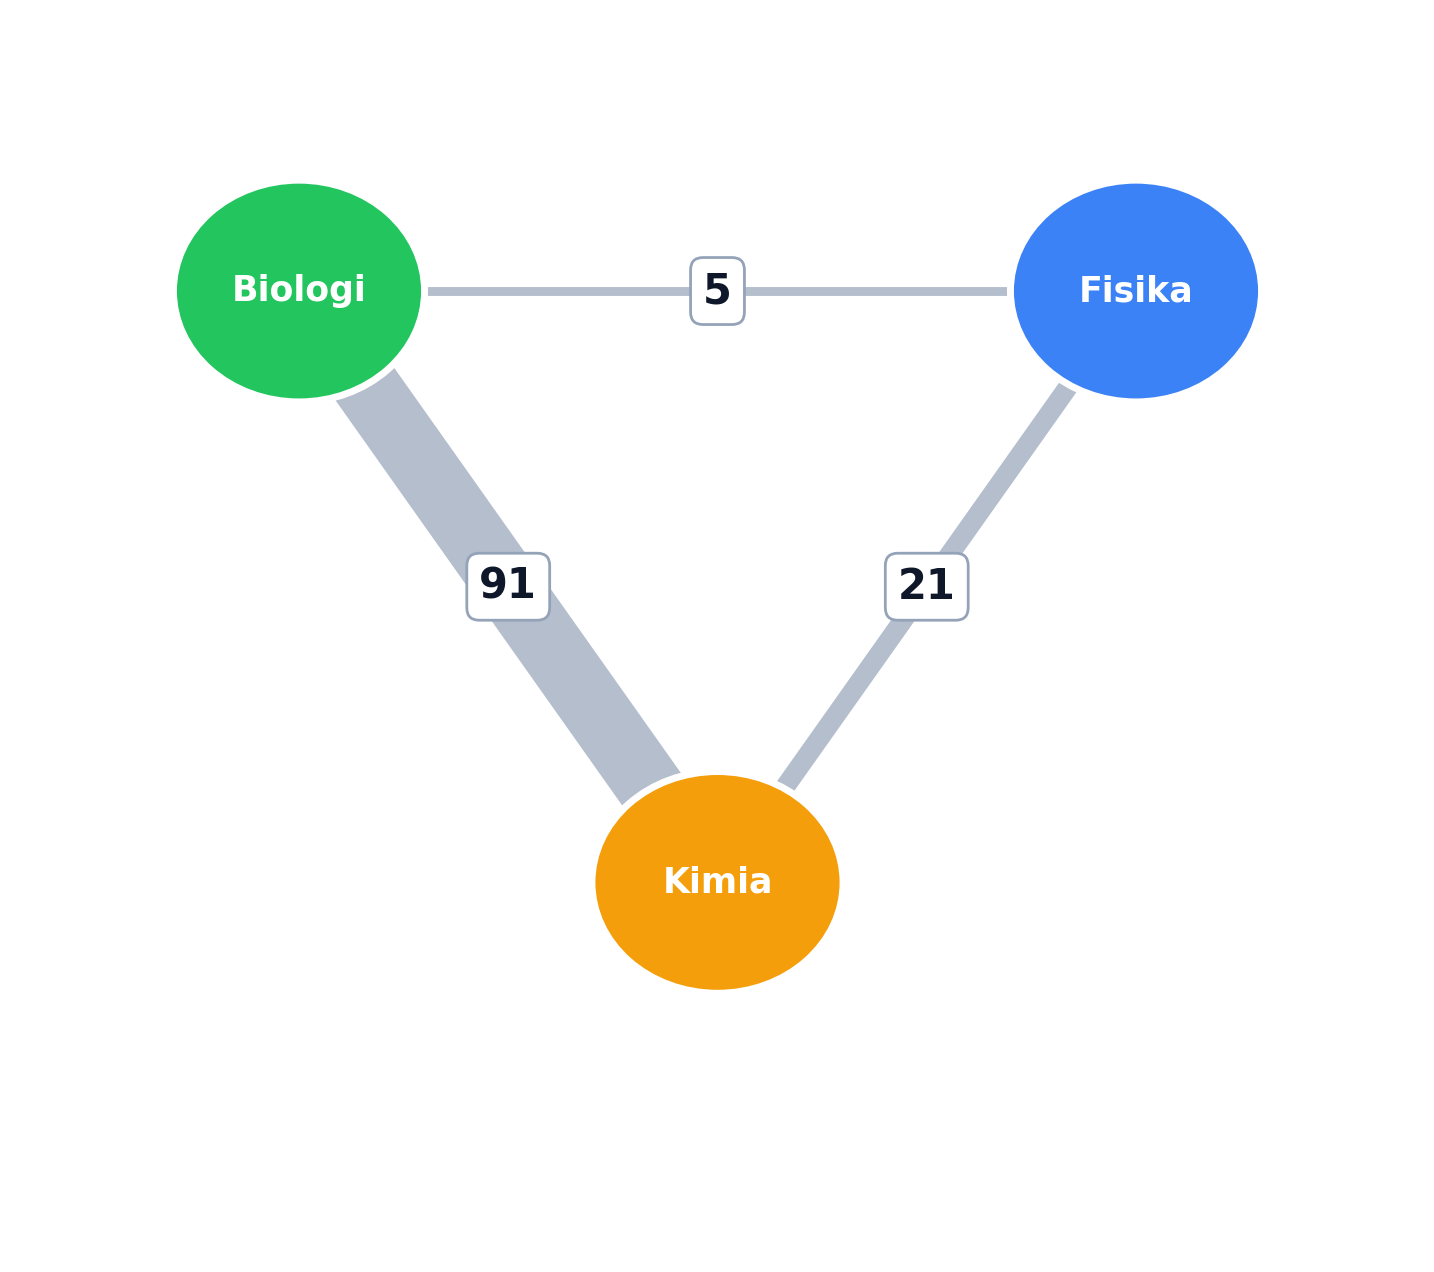
\includegraphics[width=4.39375in,height=3.33333in]{images/media/image14.png}

\textbf{Gambar 4.x} --- \emph{Inter-domain bridge graph}. Setiap simpul
adalah satu mata pelajaran; ketebalan dan label sisi menyatakan jumlah
relasi lintas-buku (LINTAS\_BUKU) yang ditemukan antar pasangan disiplin
(dari 117 relasi tersurvei).

Distribusi jembatan lintas-disiplin sangat tidak merata. Pasangan
Biologi--Kimia mendominasi (91 relasi, 78\%), diikuti Fisika--Kimia (21
relasi, 18\%), sedangkan Biologi--Fisika nyaris tidak terhubung (5
relasi, 4\%). Pola ini menempatkan Kimia sebagai poros (hub) yang
menjembatani kedua disiplin lain. Temuan ini konsisten secara pedagogis:
tumpang-tindih molekuler dan biokimiawi (DNA, protein, enzim, reaksi
redoks) membuat Biologi dan Kimia berbagi banyak konsep dasar, sementara
keterkaitan Fisika sebagian besar terbatas pada elektrokimia (arus dan
potensial listrik ↔ sel elektrokimia). Sifat Fisika yang lebih
abstrak-matematis menjadikannya domain paling terisolasi dalam jaringan
konsep kurikulum kelas XII.

Dari sisi kualitas ekstraksi (validasi Fase 1), terdapat perbedaan
antar-domain:

\begin{longtable}[]{@{}
  >{\raggedright\arraybackslash}p{(\columnwidth - 4\tabcolsep) * \real{0.1572}}
  >{\raggedright\arraybackslash}p{(\columnwidth - 4\tabcolsep) * \real{0.5095}}
  >{\raggedright\arraybackslash}p{(\columnwidth - 4\tabcolsep) * \real{0.3333}}@{}}
\toprule()
\begin{minipage}[b]{\linewidth}\raggedright
\textbf{Domain}
\end{minipage} & \begin{minipage}[b]{\linewidth}\raggedright
\textbf{Presisi ekstraksi (Fase 1)}
\end{minipage} & \begin{minipage}[b]{\linewidth}\raggedright
\textbf{Catatan}
\end{minipage} \\
\begin{minipage}[b]{\linewidth}\raggedright
Biologi
\end{minipage} & \begin{minipage}[b]{\linewidth}\raggedright
\textasciitilde0,95--0,97
\end{minipage} & \begin{minipage}[b]{\linewidth}\raggedright
\begin{itemize}
\item
  \begin{quote}
  paling konsisten;
  \end{quote}
\item
  \begin{quote}
  konsep deskriptif-naratif
  \end{quote}
\end{itemize}
\end{minipage} \\
\begin{minipage}[b]{\linewidth}\raggedright
Fisika
\end{minipage} & \begin{minipage}[b]{\linewidth}\raggedright
\textasciitilde0,86--0,99
\end{minipage} & \begin{minipage}[b]{\linewidth}\raggedright
\begin{itemize}
\item
  \begin{quote}
  rentang lebar
  \end{quote}
\item
  \begin{quote}
  lemah pada relasi kuantitatif/rumus
  \end{quote}
\end{itemize}
\end{minipage} \\
\begin{minipage}[b]{\linewidth}\raggedright
Kimia
\end{minipage} & \begin{minipage}[b]{\linewidth}\raggedright
\textasciitilde0,82--0,92
\end{minipage} & \begin{minipage}[b]{\linewidth}\raggedright
\begin{itemize}
\item
  \begin{quote}
  kesalahan terbanyak pada terminologi proses (mis. elektrorefining)
  \end{quote}
\end{itemize}
\end{minipage} \\
\midrule()
\endhead
\bottomrule()
\end{longtable}

Perbedaan ini selaras dengan analisis kesalahan (§4.2.3): kelemahan
utama pada Fisika adalah \textbf{under-extraction rumus} (67\% missing
triples Fisika berupa formula), sedangkan Kimia rentan pada
\textbf{pencampuran konsep teknis}. Biologi---yang materinya lebih
bersifat deskriptif---paling sesuai dengan kekuatan LLM dalam
mengekstrak struktur konseptual.

\begin{enumerate}
\def\labelenumi{\arabic{enumi}.}
\setcounter{enumi}{4}
\item ~
  \hypertarget{kesimpulan-dan-saran}{%
  \section{\texorpdfstring{\hfill\break
  KESIMPULAN DAN
  SARAN}{ KESIMPULAN DAN SARAN}}\label{kesimpulan-dan-saran}}

  \begin{enumerate}
  \def\labelenumii{\arabic{enumii}.}
  \item ~
    \hypertarget{kesimpulan}{%
    \subsection{\texorpdfstring{Kesimpulan
    }{Kesimpulan }}\label{kesimpulan}}
  \end{enumerate}
\end{enumerate}

Lorem ipsum dolor sit amet, consectetur adipiscing elit, sed do eiusmod
tempor incididunt ut labore et dolore magna aliqua. Ut enim ad minim
veniam, quis nostrud exercitation ullamco laboris nisi ut aliquip ex ea
commodo consequat. Duis aute irure dolor in reprehenderit in voluptate
velit esse cillum dolore eu fugiat nulla pariatur. Excepteur sint
occaecat cupidatat non proident, sunt in culpa qui officia deserunt
mollit anim id est laborum

\begin{enumerate}
\def\labelenumi{\arabic{enumi}.}
\item
  Lorem ipsum dolor sit amet, consectetur adipiscing elit, sed do
  eiusmod tempor incididunt ut labore et dolore magna aliqua.
\item
  Ut enim ad minim veniam, quis nostrud exercitation ullamco laboris
  nisi ut aliquip ex ea commodo consequat.
\item
  Duis aute irure dolor in reprehenderit in voluptate velit esse cillum
  dolore eu fugiat nulla pariatur. Excepteur sint occaecat cupidatat non
  proident, sunt in culpa qui officia deserunt mollit anim id est
  laborum
\end{enumerate}

\hypertarget{saran}{%
\subsection{Saran}\label{saran}}

Lorem ipsum dolor sit amet, consectetur adipiscing elit, sed do eiusmod
tempor incididunt ut labore et dolore magna aliqua. Ut enim ad minim
veniam, quis nostrud exercitation ullamco laboris nisi ut aliquip ex ea
commodo consequat. Duis aute irure dolor in reprehenderit in voluptate
velit esse cillum dolore eu fugiat nulla pariatur. Excepteur sint
occaecat cupidatat non proident, sunt in culpa qui officia deserunt
mollit anim id est laborum

\begin{enumerate}
\def\labelenumi{\arabic{enumi}.}
\item
  Lorem ipsum dolor sit amet, consectetur adipiscing elit, sed do
  eiusmod tempor incididunt ut labore et dolore magna aliqua.
\item
  Ut enim ad minim veniam, quis nostrud exercitation ullamco laboris
  nisi ut aliquip ex ea commodo consequat.
\item
  Duis aute irure dolor in reprehenderit in voluptate velit esse cillum
  dolore eu fugiat nulla pariatur. Excepteur sint occaecat cupidatat non
  proident, sunt in culpa qui officia deserunt mollit anim id est
  laborum
\end{enumerate}

\hypertarget{section-8}{%
\section{\texorpdfstring{\hfill\break
}{ }}\label{section-8}}

\hypertarget{daftar-pustaka}{%
\section{DAFTAR PUSTAKA}\label{daftar-pustaka}}

Amin, F. (2011). Preservasi Naskah Klasik. \emph{Journal Of Islamic
Studies}, \emph{1}.
https://jurnaliainpontianak.or.id/index.php/khatulistiwa/article/view/184/145

Bahdanau, D., Cho, K., \& Bengio, Y. (2016). \emph{Neural Machine
Translation by Jointly Learning to Align and Translate}
(arXiv:1409.0473). arXiv. http://arxiv.org/abs/1409.0473

Bird, A. (2024). \emph{Is Metadata the Key to Unlocking the Value of our
Data? \textbar{} LinkedIn}.
https://www.linkedin.com/pulse/metadata-key-unlocking-value-our-data-adam-bird-et9kc/

Dachliyani, L. (2014). \emph{Pengkatalogan Diskriptif: Bahan Ajar Teknis
Pengelolaa Perpustakaan}. Perpustakaan Nasional Republik Indonesia.

Habash, F. (2023, September 11). \emph{How AI Is Changing the
Translation Service Industry in 2024}. Localization Services by BLEND.
https://www.getblend.com/blog/artificial-intelligence-changing-the-translation-services-industry/

Kirsten, M., \& Rachel, M. (2020, December 9). \emph{Handwriting,
context and archival transcription}. Unique and Distinctive.
https://specialcollections.ul.ie/research-diaries-transcription/

Lewis, D. (2016). \emph{How Experts Are Digitizing Ancient Manuscripts}.
Smithsonian Magazine.
https://www.smithsonianmag.com/smart-news/how-experts-are-digitizing-ancient-manuscripts-180960685/

NEURODATA. (2023). \emph{How Artificial Intelligence Gives OCR a Boost
\textbar{} LinkedIn}.
https://www.linkedin.com/pulse/how-artificial-intelligence-gives-ocr-boost-neurodata/

Republik Indonesia. (2007). \emph{Undang-Undang Republik Indonesia Nomor
43 Tahun 2007 tentang Perpustakaan}.
https://peraturan.bpk.go.id/Home/Details/39889/uu-no-43-tahun-2007

Sinthuja, M., Padubidri, C. G., Jayachandra, G. S., Teja, M. C., \&
Kumar, G. S. P. (2024). Extraction of Text from Images Using Deep
Learning. \emph{Procedia Computer Science}, \emph{235}, 789--798.
https://doi.org/10.1016/j.procs.2024.04.075

Wakhid, A. (2020). \emph{Point Kebijakan Pusat Preservasi dan
Pelestarian Bahan Pustaka}.
https://preservasi.perpusnas.go.id/artikel/167/poin-kebijakan-pusat-preservasi-dalam-pelestarian-bp

Weatherall, C. (2023). \emph{Library: Archival Skills: Transcription}.
https://libguides.hull.ac.uk/archival-skills/transcription

Xu, J. (2023). The Chinese-English Translation of Four-character Pattern
from the Perspective of Functional Equivalence Theory.
\emph{Communications in Humanities Research}, \emph{3}(1), 723--728.
https://doi.org/10.54254/2753-7064/3/20220595

\protect\hypertarget{_4moq2jbvxxm5}{}{}\textbf{Lampiran 1 surat izin
penelitian}

\protect\hypertarget{_raokolpcgoou}{}{}\textbf{Lampiran 2 kuisioner}

\protect\hypertarget{_uh6gz9aal5m}{}{}\textbf{Lampiran 3 data}

\end{document}
